\documentclass[11pt]{article}
\pdfoutput=1
\usepackage{etoolbox,verbatim}
\usepackage{subcaption}
\newtoggle{arxiv}
\toggletrue{arxiv}
\newtoggle{colt}
\togglefalse{colt}
\newtoggle{iclr}
\togglefalse{iclr}
\newtoggle{customthms}
\toggletrue{customthms}
\iftoggle{iclr}{
\usepackage{iclr2026_conference,times}
}{}

%!TEX root = ../main.tex


%% macros and formating files
%!TEX root = ../main.tex


%Definitions of colors used in links, bolds, and theorem statements

\usepackage{xcolor}
\usepackage{tcolorbox}
\tcbuselibrary{skins,breakable}

\tcbset{
  aibox/.style={
      width=\linewidth,
      top=6pt,
      bottom=0pt,
      left=1.5pt,
      right=1.5pt,
colback=blue!60!gray!5,
colframe=black,
colbacktitle=black,
      enhanced,
      center,
      attach boxed title to top left={yshift=-0.1in,xshift=0.15in},
      boxed title style={boxrule=0pt,colframe=white,},
    }
}
\newtcolorbox{AIbox}[2][]{aibox,title=#2,#1}

\definecolor{primalcolor}{HTML}{A60000}
\definecolor{contrarycolor}{HTML}{00A6A6}
\definecolor{darkcontrarycolor}{HTML}{004C4C}
% \definecolor{purpleblend}{HTML}{800080}
\definecolor{lightblue}{HTML}{2970CC}
\definecolor{lightpurple}{HTML}{673147}
\definecolor{ForestGreen}{HTML}{FF5733}
\definecolor{myred}{HTML}{AA4A44}
\definecolor{hyppurple}{HTML}{800080}
\newcommand{\niceblue}{blue!60!black}
\newcommand{\linkcolor}{darkcontrarycolor}
\newcommand{\urlcolor}{darkcontrarycolor}
\newcommand{\citecolor}{darkcontrarycolor}

%{blue!70!black}
\newcommand{\thmcolor}{red!60!black}
\newcommand{\thmcolordark}{red!30!black}

\newcommand{\termcolordark}{red!65!black}
\newcommand{\termbold}[1]{{\color{\termcolordark} {\textbf{#1}}}}

\newcommand{\takeawaycolor}{red!40!black}
\newcommand{\takeawaybold}[1]{{\color{\takeawaycolor} {\textbf{#1}}}}
%!TEX root = ../main.tex

%% Fonts 
\newcommand\hmmax{0}
\newcommand\bmmax{0}
\usepackage[T1]{fontenc}
\usepackage{capt-of}
\usepackage[font=small,labelfont=bf]{caption}

%% Table of Contents

\newcommand{\nonumsection}[1]{\section*{#1}%
\addcontentsline{toc}{section}{#1}}
\newcommand{\nonumpart}[1]{\part*{#1}
\addcontentsline{toc}{part}{#1}}

%% Basic Packages

\usepackage{natbib}
\usepackage{amssymb,upgreek,bm}
\usepackage{mathtools}
\usepackage[english]{babel}  
\usepackage{multirow,tcolorbox,tikz-cd,turnstile,xspace,xparse}
\usepackage{relsize,breakcites,appendix}
\usepackage{longtable,tablefootnote,booktabs,float,makecell}
\usepackage[normalem]{ulem}
\usepackage{tabu}
\usepackage[shortlabels]{enumitem} 
\usepackage{footnote}
\usepackage{boxedminipage}
\usepackage{multirow,nicefrac}
\usepackage{verbatim} % gives the comment environment
\usepackage{wrapfig}


\usepackage[colorlinks=true,linkcolor=\linkcolor,urlcolor=\urlcolor,citecolor=\citecolor,breaklinks]{hyperref}

%% load after hyperref
\usepackage{prettyref}
\newcommand{\pref}[1]{\prettyref{#1}}
\usepackage[capitalise,nameinlink]{cleveref}

%For non-COLT papers, we add in theorem commands
\iftoggle{colt}{
    \DeclareRobustCommand{\qed}{
    %
        \usepackage{thmtools}
          \ifmmode \mathqed
          \else
            \leavevmode\unskip\penalty9999 \hbox{}\nobreak\hfill
            \quad\hbox{\qedsymbol}%
          \fi
    }
}
{
    \usepackage{amsthm}
     
}
\usepackage{thm-restate}


%% ArXiv formatting

\iftoggle{arxiv}
{
    \usepackage{mathrsfs}
    \usepackage[margin=2cm]{geometry}
    \usepackage[bitstream-charter]{mathdesign}
    \let\circledS\undefined 
    \usepackage[scaled=0.92]{PTSans}

    \usepackage{subfig}
  
  
    \renewcommand\theadalign{bc}
    \renewcommand\theadfont{\bfseries}
    \renewcommand\theadgape{\Gape[4pt]}
    \renewcommand\cellgape{\Gape[4pt]}
    \usepackage{fullpage}
    \usepackage[noend]{algpseudocode}
    \usepackage{algorithm}
   
}
{
    \usepackage{mathrsfs}
}

\DeclareMathAlphabet{\mathbfsf}{\encodingdefault}{\sfdefault}{bx}{n}

\numberwithin{equation}{section}
\newcommand\numberthis{\addtocounter{equation}{1}\tag{\theequation}}

%formatting
\iftoggle{arxiv}
{
    \newcommand{\colorbold}[1]{
    \textbf{\textcolor{\thmcolor}{#1}}}}
{
    \newcommand{\colorbold}[1]{\textbf{#1}
}
}
\iftoggle{arxiv}
{
    \newcommand{\colorpar}[1]{
    \paragraph{\textcolor{\thmcolor}{#1}}}
}
{
    \newcommand{\colorpar}[1]{\paragraph{#1}}
}



%!TEX root = ../main.tex

\usepackage{thmtools}

\Crefname{equation}{Eq.}{Eqs.}
\Crefname{assumption}{Assumption}{Assumptions}
\Crefname{condition}{Condition}{Conditions}
\Crefname{claim}{Claim}{Claims}
\Crefname{property}{Property}{Properties}
\Crefname{construction}{Construction}{Constructions}



\declaretheoremstyle[
    headformat=\normalfont\textcolor{\thmcolordark}{\bfseries\NAME\,\NUMBER}\NOTE,%
    notefont={\normalfont\textcolor{\thmcolordark}{\bfseries}}, 
    notebraces={}{},
    bodyfont=\normalfont\itshape,
    spaceabove = 6pt,
    spacebelow = 6pt,
    ]{coloredthmversion}

\declaretheoremstyle[
    headformat=\normalfont\textcolor{\thmcolordark}{\bfseries\NAME\,\NUMBER}\NOTE,%
    bodyfont=\normalfont\itshape,
    spaceabove = 6pt,
    spacebelow = 6pt,
    ]{coloredthm}

\declaretheoremstyle[
    headformat=\normalfont\textcolor{\thmcolordark}{\bfseries\NAME\,\NUMBER}\NOTE,%
    bodyfont=\normalfont,
    spaceabove = 6pt,
    spacebelow = 6pt,
    ]{coloreddef}

%Informal Theorems
\iftoggle{customthms}
{
    \theoremstyle{coloredthmversion}
}
{}
\newtheorem*{thminformalversion}{Informal Version of}



\iftoggle{customthms}{
  \theoremstyle{coloredthm}
  \newtheorem{theorem}{Theorem}
  \newtheorem{lemma}{Lemma}[section]
  \newtheorem{corollary}{Corollary}[section]
  \newtheorem{proposition}[lemma]{Proposition}
}
{}

\newtheorem{claim}[lemma]{Claim}
\newtheorem{thminformal}{Informal Theorem}
\newtheorem*{thminformal*}{Informal Theorem}
\newtheorem{oracle}{Oracle}[section]

\newtheorem{openq}{Open Question}
\newtheorem{fact}[lemma]{Fact}
\newtheorem{problem}{Problem}[section]
\newtheorem{question}{Question}[section]
\newtheorem{conjecture}{Conjecture}[section]

\newtheorem{goal}{Goal}[section]
\iftoggle{customthms}{
    \theoremstyle{coloreddef}
    \newtheorem{definition}{Definition}[section]
    \newtheorem{component}{Component}
    \newtheorem{example}{Example}[section]
    \newtheorem{remark}{Remark}[section]
    \newtheorem{property}{Property}[section]
    \newtheorem{contribution}{Contribution}
}
{
  \newtheorem{property}{Property}[section]
}

\newtheorem{observation}[lemma]{Observation}
\newtheorem{construction}{Construction}[section]


\newtheorem{assumption}{Assumption}[section]
\newtheorem{condition}{Condition}[section]

\makeatletter
\newcommand{\neutralize}[1]{\expandafter\let\csname c@#1\endcsname\count@}
\makeatother



%%%Informal Theorems
\iftoggle{customthms}{
    \newtheoremstyle{named}{}{}{\itshape}{}{\bfseries}{}{.5em}{\Cref{#3} {\normalfont (informal)} }{}
    \theoremstyle{named}
    \newtheorem*{informaltheorem}{Theorem}
    \theoremstyle{plain}
}
{}

\newenvironment{repthm}[2][]{%
  \def\theoremauxref{\cref{#2}}
  \begin{theoremaux}[#1]
}{%
  \end{theoremaux}
}


% Modified Theorems

\newenvironment{lemmod}[2]
  {\renewcommand{\thelemma}{\ref*{#1}#2}%
   \neutralize{lemma}\phantomsection
   \begin{lemma}}
  {\end{lemma}}


\newenvironment{thmmod}[3]
  {\renewcommand{\thetheorem}{\ref*{#1}#2}%
   \neutralize{theorem}\phantomsection
   \begin{theorem}[#3]}
  {\end{theorem}}


    \newenvironment{propmod}[2]
  {\renewcommand{\theproposition}{\ref*{#1}#2}%
   \neutralize{proposition}\phantomsection
   \begin{proposition}}
  {\end{proposition}}

     \newenvironment{defnmod}[2]
  {\renewcommand{\thedefinition}{\ref*{#1}#2}%
   \neutralize{definition}\phantomsection
   \begin{definition}}
  {\end{definition}}

   \newenvironment{asmmod}[2]
  {\renewcommand{\theassumption}{\ref*{#1}#2}%
   \neutralize{assumption}\phantomsection
   \begin{assumption}}
  {\end{assumption}}

  \newenvironment{cormod}[2]
  {\renewcommand{\thecorollary}{\ref*{#1}#2}%
   \neutralize{corollary}\phantomsection
   \begin{corollary}}
  {\end{corollary}}
  
   \newenvironment{condmod}[2]
  {\renewcommand{\thecondition}{\ref*{#1}#2}%
   \neutralize{condition}\phantomsection
   \begin{condition}}
  {\end{condition}}

%Unlabeled Theorems
\newtheorem*{theorem*}{Theorem}
\newtheorem*{lemma*}{Lemma}
\newtheorem*{corollary*}{Corollary}
\newtheorem*{proposition*}{Proposition}
\newtheorem*{claim*}{Claim}
\newtheorem*{fact*}{Fact}
\newtheorem*{observation*}{Observation}
\newtheorem*{definition*}{Definition}
\newtheorem*{remark*}{Remark}
\newtheorem*{example*}{Example}

%!TEX root = ../main.tex


%Bold characters
\newcommand{\bzero}{\ensuremath{\mathbf 0}}
\def\bb{\mathbf{b}}
%\def\bc{\mathbf{c}}
\def\bB{\mathbf{B}}
\def\bC{\mathbf{C}}
%\def\be{\mathbf{e}}
\def\etil{\tilde{\mathbf{e}}}
%\def\bk{\mathbf{k}}
\def\bu{\mathbf{u}}
\def\x{\mathbf{x}}
\def\y{\mathbf{y}}
\def\w{\mathbf{w}}
\def\by{\mathbf{y}}
\def\bz{\mathbf{z}}
\def\bp{\mathbf{p}}
\def\bq{\mathbf{q}}
\def\br{\mathbf{r}}
\def\bu{\mathbf{u}}
\def\bv{\mathbf{v}}

\def\bw{\mathbf{w}}
%\def\ba{\mathbf{a}}
\def\bA{\mathbf{A}}
\def\bS{\mathbf{S}}
\def\bG{\mathbf{G}}
\def\bI{\mathbf{I}}
\def\bJ{\mathbf{J}}
\def\bP{\mathbf{P}}
\def\bQ{\mathbf{Q}}
\def\bV{\mathbf{V}}
\def\bone{\mathbf{1}}

% Special letters: blackboard, mathcal, widehat % djhsu magic
\def\ddefloop#1{\ifx\ddefloop#1\else\ddef{#1}\expandafter\ddefloop\fi}
\def\ddef#1{\expandafter\def\csname bb#1\endcsname{\ensuremath{\mathbb{#1}}}}
\ddefloop ABCDEFGHIJKLMNOPQRSTUVWXYZ\ddefloop

\def\ddefloop#1{\ifx\ddefloop#1\else\ddef{#1}\expandafter\ddefloop\fi}
\def\ddef#1{\expandafter\def\csname frak#1\endcsname{\ensuremath{\mathfrak{#1}}}}
\ddefloop ABCDEFGHIJKLMNOPQRSTUVWXYZ\ddefloop

\def\ddefloop#1{\ifx\ddefloop#1\else\ddef{#1}\expandafter\ddefloop\fi}
\def\ddef#1{\expandafter\def\csname fr#1\endcsname{\ensuremath{\mathfrak{#1}}}}
\ddefloop ABCDEFGHIJKLMNOPQRSTUVWXYZ\ddefloop


\def\ddefloop#1{\ifx\ddefloop#1\else\ddef{#1}\expandafter\ddefloop\fi}
\def\ddef#1{\expandafter\def\csname eul#1\endcsname{\ensuremath{\EuScript{#1}}}}
\ddefloop ABCDEFGHIJKLMNOPQRSTUVWXYZ\ddefloop


\def\ddefloop#1{\ifx\ddefloop#1\else\ddef{#1}\expandafter\ddefloop\fi}
\def\ddef#1{\expandafter\def\csname scr#1\endcsname{\ensuremath{\mathscr{#1}}}}
\ddefloop ABCDEFGHIJKLMNOPQRSTUVWXYZ\ddefloop

\def\ddefloop#1{\ifx\ddefloop#1\else\ddef{#1}\expandafter\ddefloop\fi}
\def\ddef#1{\expandafter\def\csname b#1\endcsname{\ensuremath{\mathbf{#1}}}}
\ddefloop ABCDEFGHIJKLMNOPQRSTUVWXYZ\ddefloop


\def\ddefloop#1{\ifx\ddefloop#1\else\ddef{#1}\expandafter\ddefloop\fi}
\def\ddef#1{\expandafter\def\csname bhat#1\endcsname{\ensuremath{\hat{\mathbf{#1}}}}}
\ddefloop ABCDEFGHIJKLMNOPQRSTUVWXYZ\ddefloop

\def\ddefloop#1{\ifx\ddefloop#1\else\ddef{#1}\expandafter\ddefloop\fi}
\def\ddef#1{\expandafter\def\csname btil#1\endcsname{\ensuremath{\tilde{\mathbf{#1}}}}}
\ddefloop ABCDEFGHIJKLMNOPQRSTUVWXYZ\ddefloop

\def\ddefloop#1{\ifx\ddefloop#1\else\ddef{#1}\expandafter\ddefloop\fi}
\def\ddef#1{\expandafter\def\csname bst#1\endcsname{\ensuremath{\mathbf{#1}^\star}}}
\ddefloop ABCDEFGHIJKLMNOPQRSTUVWXYZ\ddefloop

\def\ddefloop#1{\ifx\ddefloop#1\else\ddef{#1}\expandafter\ddefloop\fi}
\def\ddef#1{\expandafter\def\csname bst#1\endcsname{\ensuremath{\mathbf{#1}^\star}}}
\ddefloop abcdeghijklmnopqrstuvwxyz\ddefloop

\def\ddefloop#1{\ifx\ddefloop#1\else\ddef{#1}\expandafter\ddefloop\fi}
\def\ddef#1{\expandafter\def\csname bhat#1\endcsname{\ensuremath{\hat{\mathbf{#1}}}}}
\ddefloop abcdefghijklmnopqrstuvwxyz\ddefloop

% no \bm
\def\ddefloop#1{\ifx\ddefloop#1\else\ddef{#1}\expandafter\ddefloop\fi}
\def\ddef#1{\expandafter\def\csname b#1\endcsname{\ensuremath{\mathbf{#1}}}}
\ddefloop abcdeghijklnopqrstuvwxyz\ddefloop

\def\ddefloop#1{\ifx\ddefloop#1\else\ddef{#1}\expandafter\ddefloop\fi}
\def\ddef#1{\expandafter\def\csname barb#1\endcsname{\ensuremath{\bar{\mathbf{#1}}}}}
\ddefloop abcdefghijklmnopqrstuvwxyz\ddefloop

\def\ddef#1{\expandafter\def\csname c#1\endcsname{\ensuremath{\mathcal{#1}}}}
\ddefloop ABCDEFGHIJKLMNOPQRSTUVWXYZ\ddefloop
\def\ddef#1{\expandafter\def\csname h#1\endcsname{\ensuremath{\widehat{#1}}}}
\ddefloop ABCDEFGHIJKLMNOPQRSTUVWXYZ\ddefloop
\def\ddef#1{\expandafter\def\csname hc#1\endcsname{\ensuremath{\widehat{\mathcal{#1}}}}}
\ddefloop ABCDEFGHIJKLMNOPQRSTUVWXYZ\ddefloop
\def\ddef#1{\expandafter\def\csname t#1\endcsname{\ensuremath{\widetilde{#1}}}}
\ddefloop ABCDEFGHIJKLMNOPQRSTUVWXYZ\ddefloop
\def\ddef#1{\expandafter\def\csname tc#1\endcsname{\ensuremath{\widetilde{\mathcal{#1}}}}}
\ddefloop ABCDEFGHIJKLMNOPQRSTUVWXYZ\ddefloop
%!TEX root = ../main.tex

%Text Formatting
\newcommand{\email}[1]{\texttt{#1}}
\newcommand{\sftext}[1]{{\normalfont \textsf{#1}}}
\newcommand{\normtext}[1]{{\normalfont \text{#1}}}
\newcommand{\algcomment}[1]{\texttt{\color{blue} #1}}
\newcommand{\textnorm}[1]{\text{\normalfont #1}}
\newcommand{\mb}[1]{\mathbf{#1}}
\newcommand{\FigureOut}{{\color{blue} (\mathrm{FigureOut}) }}
\newcommand{\dbtilde}[1]{\tilde{\raisebox{0pt}[0.85\height]{$\tilde{#1}$}}}
\newcommand{\newlytyped}[1]{{\color{green}#1}}
\newcommand{\remind}[1]{{\color{blue}#1}}

%% Delimiters

\DeclarePairedDelimiter{\abs}{\lvert}{\rvert} %
\DeclarePairedDelimiter{\brk}{[}{]}
\DeclarePairedDelimiter{\crl}{\{}{\}}
\DeclarePairedDelimiter{\prn}{(}{)}
\DeclarePairedDelimiter{\nrm}{\|}{\|}
\DeclarePairedDelimiter{\tri}{\langle}{\rangle}
\DeclarePairedDelimiter{\dtri}{\llangle}{\rrangle}
\newcommand{\ceil}[1]{\lceil #1 \rceil}
\newcommand{\floor}[1]{\lfloor #1 \rfloor}

%% Decorators 

\renewcommand{\t}[1]{\smash{\tilde{#1}}}
\newcommand{\wt}[1]{\smash{\widetilde{#1}}}
\newcommand{\wh}[1]{\smash{\widehat{#1}}}
\newcommand{\OO}[1]{\O\lr{#1}}
\newcommand{\tTheta}{\wt{\Theta}}

%% Operators

\newcommand{\I}{\mathbf{I}}
\newcommand{\tsum}{\sum\nolimits}
\newcommand{\ind}[1]{\mathbb{I}\!\lrset{#1}}
\newcommand{\non}{\nonumber}
\DeclareMathOperator*{\argmin}{arg\,min}
\DeclareMathOperator*{\argmax}{arg\,max}
\DeclareMathOperator*{\conv}{conv}
\DeclareMathOperator*{\supp}{supp}



%% Asymptotics

\newcommand{\poly}{\mathrm{poly}}
\newcommand{\BigOhSt}[1]{\BigOm^*\left({#1}\right)}
\DeclareMathOperator{\BigOm}{{O}}
\newcommand{\BigOhPar}[2] {\BigOm_{#1}\left({#2}\right)}
\newcommand{\BigOh}[1]{\BigOm\left({#1}\right)}
\DeclareMathOperator{\BigOmtil}{\widetilde{\mathcal{O}}}
\newcommand{\BigOhTil}[1]{\BigOmtil\left({#1}\right)}
\DeclareMathOperator{\BigTm}{\Theta}
\newcommand{\BigTheta}[1]{\BigTm\left({#1}\right)}
\DeclareMathOperator{\BigWm}{\Omega}
\newcommand{\BigThetaTil}[1]{\widetilde{\BigTm}\left({#1}\right)}
\newcommand{\BigOmega}[1]{\BigWm\left({#1}\right)}
\newcommand{\BigOmegaSt}[1]{\BigWm^*\left({#1}\right)}
\newcommand{\BigOmegaTil}[1]{\widetilde{\BigWm}\left({#1}\right)}
\newcommand{\bigohst}[1]{\mathcal{O}(#1)}
\newcommand{\bigomst}[1]{\Omega(#1)}



%% Probability and Measure Theory

\let\Pr\relax
\DeclareMathOperator{\Pr}{\mathbb{P}}
\DeclareMathOperator*{\Expop}{\mathbb{E}}
\newcommand{\E}{\mathbb{E}}
\newcommand{\Exp}{\mathbb{E}}
\newcommand{\EE}[1]{\E\lrbra{#1}}
\newcommand{\var}{\mathrm{Var}}
\newcommand{\Leb}{\mathrm{Leb}}
\newcommand{\Unif}{\Dist_{\mathrm{unif}}}
\newcommand{\Normal}{\mathrm{N}}
\newcommand{\iidsim}{\overset{\mathrm{i.i.d}}{\sim}}


%% Linear Algebra

\newcommand{\eye}{\mathbf{I}}
\newcommand{\trn}{\intercal}
\renewcommand{\sp}{\mathrm{span}}
\newcommand{\trace}{\mathrm{tr}}



%% Metric Space Quantities

\newcommand{\ballk}[1][k]{\cB_{#1}}
\newcommand{\ballkr}[1][r]{\cB_{k}(r)}
\newcommand{\op}{\mathrm{op}}
\newcommand{\fro}{\mathrm{F}}


%% Differential Operators

\def\hestinv{\tilde{\nabla}^{-2}}
\def\hest{\tilde{\nabla}^{2}}
\def\hessinv{\nabla^{-2}}
\def\hess{\nabla^2}
\def\grad{\nabla}
\newcommand{\nablatwo}{\nabla^{\,2}}
\def\ntil{\tilde{\nabla}}
\newcommand{\rmd}{\mathrm{d}}
\newcommand{\Diag}{\mathrm{Diag}}% notation
\newcommand{\Differential}{\mathsf{D}}
\newcommand{\re}{{\text{Re}}}

%%Statistical Learning

\newcommand{\fst}{f^\star}
\newcommand{\gst}{g^\star}
\newcommand{\Gclass}{\cG}
\newcommand{\Regret}{\mathrm{Regret}}
\def\regret{\mbox{{Regret\ }}}
\newcommand{\ftil}{\tilde{f}}
\newcommand{\mH}{\mathcal{H}}
\def\X{{\mathcal X}}
\def\U{{\mathcal U}}
\def\H{{\mathcal H}}
\def\Y{{\mathcal Y}}



%% Logical Operators

\newcommand{\True}{\mathsf{True}}
\newcommand{\False}{\mathsf{False}}

%% Assorted Characters

\newcommand{\nicehalf}{\nicefrac{1}{2}}
\newcommand{\veps}{\varepsilon}
\DeclareMathSymbol{\shortminus}{\mathbin}{AMSa}{"39}
\newcommand{\N}{\mathbb{N}}
\newcommand{\R}{\mathbb{R}}
\newcommand{\defeq}{:=}
\def\ytil{\tilde{{y}}}
\def\yhat{\hat{{y}}}
\def\what{\hat{{\bw}}}
\def\xhat{\hat{\mathbf{x}}}
\def\xbar{\bar{\mathbf{x}}}






%% Cases

\newcommand{\mycases}[4]{{
\left\{
\begin{array}{ll}
    {#1} & {\;\text{#2}} \\[1ex]
    {#3} & {\;\text{#4}}
\end{array}
\right. }}

\newcommand{\mythreecases}[6] {{
\left\{
\begin{array}{ll}
    {#1} & {\;\text{#2}} \\[1ex]
    {#3} & {\;\text{#4}} \\[1ex]
    {#5} & {\;\text{#6}}
\end{array}
\right. }}

%%% Deprecated

    %\newcommand{\lrp}[1]{\!\left(#1\right)\!}
    %\newcommand{\lrbig}[1]{\big(#1\big)}
    %\newcommand{\lrBig}[1]{\Big(#1\Big)}
    %\newcommand{\lrbra}[1]{\!\left[#1\right]\!}
    %\newcommand{\lrnorm}[1]{\left\|#1\right\|}
    %\newcommand{\lrset}[1]{\left\{#1\right\}}
    %\newcommand{\lrabs}[1]{\left|#1\right|}
    %\newcommand{\norm}[1]{\|#1\|}
%!TEX root = ../main.tex

% Custom ref commands
\Crefname{component}{Component}{Components}
\Crefname{contribution}{Contribution}{Contributions}
\newcommand{\componentref}[1]{%
  \hyperref[#1]{C\ref*{#1}}%
}
\Crefname{claim}{Claim}{Claims}
\Crefname{property}{Property}{Properties}

% Hypothesis commands
\newcommand{\hyp}[1]{{\color{hyppurple}{H#1}}}
\newcommand{\hypanchor}[1]{\hypertarget{hyp:#1}{\hyp{#1}}} % place anchor
\newcommand{\hypref}[1]{\hyperlink{hyp:#1}{\hyp{#1}}}     % clickable reference

% ICLR paragraph formatting
\newcommand{\iclrpar}[1]{\paragraph{\takeawaybold{#1}}}

% ICLR style for equations (smaller text in ICLR format)
\iftoggle{iclr}
{
  \newcommand{\iclrstyle}{\textstyle}
}
{
  \newcommand{\iclrstyle}{}
}

% Theorem text formatting
\newcommand{\thmbolddark}[1]{{\color{\thmcolordark}\textbf{#1}}}

% Math operators
\newcommand{\stopgrad}{\mathrm{sg}}

\newcommand{\flowpol}{\pi}
\newcommand{\piideal}{\pi^{\star}}
\newcommand{\flowideal}{b^{\star}}

\newcommand{\Gsmooth}{\cG_{\mathrm{smooth}}}
\newcommand{\fbar}{\bar{f}}
\newcommand{\beps}{\bm{\epsilon}}
\newcommand{\betabar}{\bar{\beta}}
\newcommand{\minprobcost}[1][\cost]{\minmax_{#1,\mathrm{prob}}}
\newcommand{\sampreg}[1][n]{S_{#1,\mathrm{reg}}}
\newcommand{\regfam}{$k$-dimensional regression problem class}
\newcommand{\kappaconc}{\kappa}
\newcommand{\deltaconc}{\delta}
\newcommand{\nconc}{n_{0}}
\newcommand{\Var}{\mathrm{Var}}
\newcommand{\Disz}[1][z]{\Dist_{\{Z=#1\}}}
\newcommand{\angs}[2]{\left \langle #1,#2 \right \rangle}
\newcommand{\absangs}[2]{\left|\left \langle #1,#2 \right \rangle\right|}

\newcommand{\ddt}{\frac{\rmd }{\rmd t}}
\renewcommand{\Normal}{\mathrm{N}}

\newcommand{\Dist}{D}

% Metadata commands (inspired by fairmeta.cls)
\makeatletter
% Helper command to add items to a list
\newcommand\addtometadatalist[5][]{%
  \begingroup
  \if\relax#3\relax\def\sep{}\else\def\sep{#5}\fi
  \let\protect\@unexpandable@protect
  \xdef#3{\expandafter{#3}\sep #4[#1]{#2}}%
  \endgroup
}

% Metadata list and format
\newcommand\metadatalist{}
\newcommand\metadataformat[2][]{{\small \textbf{#1:} #2}}
\newcommand\metadata[2][]{\addtometadatalist[#1]{#2}{\metadatalist}{\metadataformat}{\\}}
\makeatother

% Convenience commands for common metadata
\newcommand{\paperwebsite}[1]{\metadata[Website]{\url{#1}}}
\newcommand{\papercode}[1]{\metadata[Code]{\url{#1}}}
\newcommand{\paperdocs}[1]{\metadata[Documentation]{\url{#1}}}
\newcommand{\paperblog}[1]{\metadata[Blog]{\url{#1}}}
%!TEX root = ../main.tex

% Commands from old algnames.tex
\newcommand{\taskname}[1]{{\texttt{#1}}}
\newcommand{\algname}[1]{\textbf{\texttt{#1}}}
\newcommand{\archname}[1]{\texttt{#1}}

% Task name commands
\newcommand{\lifttask}{\taskname{Lift}\xspace}
\newcommand{\can}{\taskname{Can}\xspace}
\newcommand{\squaretask}{\taskname{Square}\xspace}
\newcommand{\transport}{\taskname{Transport}\xspace}
\newcommand{\toolhang}{\taskname{Tool}-\taskname{Hang}\xspace}
\newcommand{\pusht}{\taskname{Push}-\taskname{T}\xspace}
\newcommand{\kitchen}{\taskname{Kitchen}\xspace}
\newcommand{\metaworld}{\taskname{MetaWorld}\xspace}
\newcommand{\adroit}{\taskname{Adroit}\xspace}
\newcommand{\toolhangphstate}{\taskname{Tool}-\taskname{Hang} \taskname{(PH,State)}\xspace}

% Algorithm name commands
\newcommand{\flow}{\algname{flow}\xspace}
\newcommand{\Flow}{\algname{Flow}\xspace}
\newcommand{\regression}{RCP\xspace}
\newcommand{\Regression}{\algname{Regression}\xspace}

\newcommand{\straightflow}{straight-flow\xspace}
\newcommand{\Straightflow}{\algname{SF}\xspace}
\newcommand{\twostagrer}{two-stage regression\xspace}
\newcommand{\Twostagrer}{\algname{TSR}\xspace}
\newcommand{\residualregression}{residual regression\xspace}
\newcommand{\Residualregression}{\algname{RR}\xspace}
\newcommand{\minimaliterativepolicy}{minimal iterative policy\xspace}
\newcommand{\mminimaliterativepolicy}{Minimal iterative policy\xspace}
\newcommand{\Minimaliterativepolicy}{\algname{MIP}\xspace}

% Architecture name commands
\newcommand{\chiunet}{\archname{Chi-UNet}\xspace}
\newcommand{\sudeepdit}{\archname{Sudeep-DiT}\xspace}
\newcommand{\chitransformer}{\archname{Chi-Transformer}\xspace}
\newcommand{\rnn}{\archname{RNN}\xspace}
\newcommand{\mlp}{\archname{MLP}\xspace}

\newcommand{\algofont}[1]{{\scalefont{1.1}{\texttt{\textbf{#1}}}}}
\newcommand{\algofonttitle}[1]{{\scalefont{1.08}{\textbf{\texttt{#1}}}}}
\newcommand{\urlfont}[1]{{\scalefont{1.0}{\texttt{\textbf{#1}}}}}

% DPPO
\newcommand{\DPPOcolor}{red!70!black}
%\newcommand{\DPPO}{\algofont{DPPO}}
\newcommand{\DPPOnc}{\algofont{DPPO}}
\newcommand{\DPPOc}{{\color{\DPPOcolor}\DPPOnc}}
\newcommand{\DPPO}{{\color{\DPPOcolor}\DPPOnc}}
\newcommand{\DPPOtitle}{{\color{\DPPOcolor}\algofonttitle{DPPO}}}

%IDQL
\newcommand{\IDQL}{\algofont{IDQL}}
\newcommand{\IDQLcolor}{black}
\newcommand{\IDQLc}{{\color{\IDQLcolor}\IDQL}}


% DRWR 
\newcommand{\DRWRcolor}{blue!60!green}
\newcommand{\DRWR}{\algofont{DRWR}}
\newcommand{\DRWRc}{{\color{\DRWRcolor}\DRWR}}


%DAWR
\newcommand{\DAWRcolor}{green!60!black}
\newcommand{\DAWR}{\algofont{DAWR}}
\newcommand{\DAWRc}{{\color{\DAWRcolor}\DAWR}}


%DIPO
\newcommand{\DIPOcolor}{gray}
\newcommand{\DIPO}{\algofont{DIPO}}
\newcommand{\DIPOc}{{\color{\DIPOcolor}\DIPO}}


%DQL
\newcommand{\DQLcolor}{magenta!80!black}
\newcommand{\DQL}{\algofont{DQL}}
\newcommand{\DQLc}{{\color{\DQLcolor}\DQL}}


%QSM
\newcommand{\QSMcolor}{yellow!70!black}
\newcommand{\QSM}{\algofont{QSM}}
\newcommand{\QSMc}{{\color{\QSMcolor}\QSM}}

%RLPD
\newcommand{\RLPDcolor}{gray!40!black}
\newcommand{\RLPD}{\algofont{RLPD}}
\newcommand{\RLPDc}{{\color{\RLPDcolor}\RLPD}}

%Cal-QL
\newcommand{\CALQLcolor}{teal!80!blue}
\newcommand{\CALQL}{\algofont{Cal-QL}}
\newcommand{\CALQLc}{{\color{\CALQLcolor}\CALQL}}

%IBRL
\newcommand{\IBRLcolor}{purple!60!black}
\newcommand{\IBRL}{\algofont{IBRL}}
\newcommand{\IBRLc}{{\color{\IBRLcolor}\IBRL}}

% Mujoco
\newcommand{\HopperEnv}{\texttt{Hopper-v2}}
\newcommand{\WalkerEnv}{\texttt{Walker2D-v2}}
\newcommand{\CheetahEnv}{\texttt{HalfCheetah-v2}}
\newcommand{\KitchenComplete}{\texttt{Kitchen-Complete-v0}}
\newcommand{\KitchenPartial}{\texttt{Kitchen-Partial-v0}}
\newcommand{\KitchenMixed}{\texttt{Kitchen-Mixed-v0}}

% Robomimic
\newcommand{\LiftEnv}{\texttt{Lift}}
\newcommand{\CanEnv}{\texttt{Can}}
\newcommand{\TransEnv}{\texttt{Transport}}
\newcommand{\SqEnv}{\texttt{Square}}

% Furniture-bench
\newcommand{\OneLegEnv}{\texttt{One-leg}}
\newcommand{\LampEnv}{\texttt{Lamp}}
\newcommand{\RoundTableEnv}{\texttt{Round-table}}

% D3IL
\newcommand{\AvoidEnv}{\texttt{Avoid}}
\newcommand{\toy}{\textsc{D3IL}}

\newcommand{\FurnitureBench}{\textsc{Furniture}-\textsc{Bench}}
\newcommand{\Robomimic}{\textsc{Robomimic}}
\newcommand{\Gym}{\textsc{Gym}}
\newcommand{\LowRand}{\texttt{Low}}
\newcommand{\MedRand}{\texttt{Med}}
\newcommand{\KitchenEnv}{\textsc{Franka}-\textsc{Kitchen}}











%% edits macros

% \usepackage{preamble_new/color-edits}
%% author names for color edits

% \addauthor{ms}{magenta}


%% General Comments

\newcommand{\REF}{{\color{red} \textbf{REF??}}}
\newcommand{\CITE}{{\color{red} \textbf{CITE??}}}
\newcommand{\TODO}{\textbf{\color{red} TODO}}
\newcommand{\ignore}[1]{}

%% titling

\iftoggle{arxiv}
{
\makeatletter
\renewcommand{\abstractname}{\normalsize Abstract}
\makeatother

\makeatletter
\renewcommand{\maketitle}{
    \newpage
    \null
    %\vskip 2em
    \begingroup
    \raggedright
    %\let\footnote\@gobble
    {\LARGE \bfseries \@title \par}
    \vskip 1.5em
        {\large
            \lineskip .5em
            \begin{tabular}[t]{l}
                \@author
            \end{tabular}\par}
    \vskip 1em
        {\large \@date \par}
    \endgroup
    \par
    \vskip 1.5em
}
\makeatother
}
{}


% %!TEX root = ../main.tex

%% Fonts 
\newcommand\hmmax{0}
\newcommand\bmmax{0}
\usepackage[T1]{fontenc}
\usepackage{capt-of}
\usepackage[font=small,labelfont=bf]{caption}

%% Table of Contents

\newcommand{\nonumsection}[1]{\section*{#1}%
\addcontentsline{toc}{section}{#1}}
\newcommand{\nonumpart}[1]{\part*{#1}
\addcontentsline{toc}{part}{#1}}

%% Basic Packages

\usepackage{natbib}
\usepackage{amssymb,upgreek,bm}
\usepackage{mathtools}
\usepackage[english]{babel}  
\usepackage{multirow,tcolorbox,tikz-cd,turnstile,xspace,xparse}
\usepackage{relsize,breakcites,appendix}
\usepackage{longtable,tablefootnote,booktabs,float,makecell}
\usepackage[normalem]{ulem}
\usepackage{tabu}
\usepackage[shortlabels]{enumitem} 
\usepackage{footnote}
\usepackage{boxedminipage}
\usepackage{multirow,nicefrac}
\usepackage{verbatim} % gives the comment environment
\usepackage{wrapfig}


\usepackage[colorlinks=true,linkcolor=\linkcolor,urlcolor=\urlcolor,citecolor=\citecolor,breaklinks]{hyperref}

%% load after hyperref
\usepackage{prettyref}
\newcommand{\pref}[1]{\prettyref{#1}}
\usepackage[capitalise,nameinlink]{cleveref}

%For non-COLT papers, we add in theorem commands
\iftoggle{colt}{
    \DeclareRobustCommand{\qed}{
    %
        \usepackage{thmtools}
          \ifmmode \mathqed
          \else
            \leavevmode\unskip\penalty9999 \hbox{}\nobreak\hfill
            \quad\hbox{\qedsymbol}%
          \fi
    }
}
{
    \usepackage{amsthm}
     
}
\usepackage{thm-restate}


%% ArXiv formatting

\iftoggle{arxiv}
{
    \usepackage{mathrsfs}
    \usepackage[margin=2cm]{geometry}
    \usepackage[bitstream-charter]{mathdesign}
    \let\circledS\undefined 
    \usepackage[scaled=0.92]{PTSans}

    \usepackage{subfig}
  
  
    \renewcommand\theadalign{bc}
    \renewcommand\theadfont{\bfseries}
    \renewcommand\theadgape{\Gape[4pt]}
    \renewcommand\cellgape{\Gape[4pt]}
    \usepackage{fullpage}
    \usepackage[noend]{algpseudocode}
    \usepackage{algorithm}
   
}
{
    \usepackage{mathrsfs}
}

\DeclareMathAlphabet{\mathbfsf}{\encodingdefault}{\sfdefault}{bx}{n}

\numberwithin{equation}{section}
\newcommand\numberthis{\addtocounter{equation}{1}\tag{\theequation}}

%formatting
\iftoggle{arxiv}
{
    \newcommand{\colorbold}[1]{
    \textbf{\textcolor{\thmcolor}{#1}}}}
{
    \newcommand{\colorbold}[1]{\textbf{#1}
}
}
\iftoggle{arxiv}
{
    \newcommand{\colorpar}[1]{
    \paragraph{\textcolor{\thmcolor}{#1}}}
}
{
    \newcommand{\colorpar}[1]{\paragraph{#1}}
}



% %!TEX root = ../main.tex


%Bold characters
\newcommand{\bzero}{\ensuremath{\mathbf 0}}
\def\bb{\mathbf{b}}
%\def\bc{\mathbf{c}}
\def\bB{\mathbf{B}}
\def\bC{\mathbf{C}}
%\def\be{\mathbf{e}}
\def\etil{\tilde{\mathbf{e}}}
%\def\bk{\mathbf{k}}
\def\bu{\mathbf{u}}
\def\x{\mathbf{x}}
\def\y{\mathbf{y}}
\def\w{\mathbf{w}}
\def\by{\mathbf{y}}
\def\bz{\mathbf{z}}
\def\bp{\mathbf{p}}
\def\bq{\mathbf{q}}
\def\br{\mathbf{r}}
\def\bu{\mathbf{u}}
\def\bv{\mathbf{v}}

\def\bw{\mathbf{w}}
%\def\ba{\mathbf{a}}
\def\bA{\mathbf{A}}
\def\bS{\mathbf{S}}
\def\bG{\mathbf{G}}
\def\bI{\mathbf{I}}
\def\bJ{\mathbf{J}}
\def\bP{\mathbf{P}}
\def\bQ{\mathbf{Q}}
\def\bV{\mathbf{V}}
\def\bone{\mathbf{1}}

% Special letters: blackboard, mathcal, widehat % djhsu magic
\def\ddefloop#1{\ifx\ddefloop#1\else\ddef{#1}\expandafter\ddefloop\fi}
\def\ddef#1{\expandafter\def\csname bb#1\endcsname{\ensuremath{\mathbb{#1}}}}
\ddefloop ABCDEFGHIJKLMNOPQRSTUVWXYZ\ddefloop

\def\ddefloop#1{\ifx\ddefloop#1\else\ddef{#1}\expandafter\ddefloop\fi}
\def\ddef#1{\expandafter\def\csname frak#1\endcsname{\ensuremath{\mathfrak{#1}}}}
\ddefloop ABCDEFGHIJKLMNOPQRSTUVWXYZ\ddefloop

\def\ddefloop#1{\ifx\ddefloop#1\else\ddef{#1}\expandafter\ddefloop\fi}
\def\ddef#1{\expandafter\def\csname fr#1\endcsname{\ensuremath{\mathfrak{#1}}}}
\ddefloop ABCDEFGHIJKLMNOPQRSTUVWXYZ\ddefloop


\def\ddefloop#1{\ifx\ddefloop#1\else\ddef{#1}\expandafter\ddefloop\fi}
\def\ddef#1{\expandafter\def\csname eul#1\endcsname{\ensuremath{\EuScript{#1}}}}
\ddefloop ABCDEFGHIJKLMNOPQRSTUVWXYZ\ddefloop


\def\ddefloop#1{\ifx\ddefloop#1\else\ddef{#1}\expandafter\ddefloop\fi}
\def\ddef#1{\expandafter\def\csname scr#1\endcsname{\ensuremath{\mathscr{#1}}}}
\ddefloop ABCDEFGHIJKLMNOPQRSTUVWXYZ\ddefloop

\def\ddefloop#1{\ifx\ddefloop#1\else\ddef{#1}\expandafter\ddefloop\fi}
\def\ddef#1{\expandafter\def\csname b#1\endcsname{\ensuremath{\mathbf{#1}}}}
\ddefloop ABCDEFGHIJKLMNOPQRSTUVWXYZ\ddefloop


\def\ddefloop#1{\ifx\ddefloop#1\else\ddef{#1}\expandafter\ddefloop\fi}
\def\ddef#1{\expandafter\def\csname bhat#1\endcsname{\ensuremath{\hat{\mathbf{#1}}}}}
\ddefloop ABCDEFGHIJKLMNOPQRSTUVWXYZ\ddefloop

\def\ddefloop#1{\ifx\ddefloop#1\else\ddef{#1}\expandafter\ddefloop\fi}
\def\ddef#1{\expandafter\def\csname btil#1\endcsname{\ensuremath{\tilde{\mathbf{#1}}}}}
\ddefloop ABCDEFGHIJKLMNOPQRSTUVWXYZ\ddefloop

\def\ddefloop#1{\ifx\ddefloop#1\else\ddef{#1}\expandafter\ddefloop\fi}
\def\ddef#1{\expandafter\def\csname bst#1\endcsname{\ensuremath{\mathbf{#1}^\star}}}
\ddefloop ABCDEFGHIJKLMNOPQRSTUVWXYZ\ddefloop

\def\ddefloop#1{\ifx\ddefloop#1\else\ddef{#1}\expandafter\ddefloop\fi}
\def\ddef#1{\expandafter\def\csname bst#1\endcsname{\ensuremath{\mathbf{#1}^\star}}}
\ddefloop abcdeghijklmnopqrstuvwxyz\ddefloop

\def\ddefloop#1{\ifx\ddefloop#1\else\ddef{#1}\expandafter\ddefloop\fi}
\def\ddef#1{\expandafter\def\csname bhat#1\endcsname{\ensuremath{\hat{\mathbf{#1}}}}}
\ddefloop abcdefghijklmnopqrstuvwxyz\ddefloop

% no \bm
\def\ddefloop#1{\ifx\ddefloop#1\else\ddef{#1}\expandafter\ddefloop\fi}
\def\ddef#1{\expandafter\def\csname b#1\endcsname{\ensuremath{\mathbf{#1}}}}
\ddefloop abcdeghijklnopqrstuvwxyz\ddefloop

\def\ddefloop#1{\ifx\ddefloop#1\else\ddef{#1}\expandafter\ddefloop\fi}
\def\ddef#1{\expandafter\def\csname barb#1\endcsname{\ensuremath{\bar{\mathbf{#1}}}}}
\ddefloop abcdefghijklmnopqrstuvwxyz\ddefloop

\def\ddef#1{\expandafter\def\csname c#1\endcsname{\ensuremath{\mathcal{#1}}}}
\ddefloop ABCDEFGHIJKLMNOPQRSTUVWXYZ\ddefloop
\def\ddef#1{\expandafter\def\csname h#1\endcsname{\ensuremath{\widehat{#1}}}}
\ddefloop ABCDEFGHIJKLMNOPQRSTUVWXYZ\ddefloop
\def\ddef#1{\expandafter\def\csname hc#1\endcsname{\ensuremath{\widehat{\mathcal{#1}}}}}
\ddefloop ABCDEFGHIJKLMNOPQRSTUVWXYZ\ddefloop
\def\ddef#1{\expandafter\def\csname t#1\endcsname{\ensuremath{\widetilde{#1}}}}
\ddefloop ABCDEFGHIJKLMNOPQRSTUVWXYZ\ddefloop
\def\ddef#1{\expandafter\def\csname tc#1\endcsname{\ensuremath{\widetilde{\mathcal{#1}}}}}
\ddefloop ABCDEFGHIJKLMNOPQRSTUVWXYZ\ddefloop
% %!TEX root = ../main.tex

% Commands from old algnames.tex
\newcommand{\taskname}[1]{{\texttt{#1}}}
\newcommand{\algname}[1]{\textbf{\texttt{#1}}}
\newcommand{\archname}[1]{\texttt{#1}}

% Task name commands
\newcommand{\lifttask}{\taskname{Lift}\xspace}
\newcommand{\can}{\taskname{Can}\xspace}
\newcommand{\squaretask}{\taskname{Square}\xspace}
\newcommand{\transport}{\taskname{Transport}\xspace}
\newcommand{\toolhang}{\taskname{Tool}-\taskname{Hang}\xspace}
\newcommand{\pusht}{\taskname{Push}-\taskname{T}\xspace}
\newcommand{\kitchen}{\taskname{Kitchen}\xspace}
\newcommand{\metaworld}{\taskname{MetaWorld}\xspace}
\newcommand{\adroit}{\taskname{Adroit}\xspace}
\newcommand{\toolhangphstate}{\taskname{Tool}-\taskname{Hang} \taskname{(PH,State)}\xspace}

% Algorithm name commands
\newcommand{\flow}{\algname{flow}\xspace}
\newcommand{\Flow}{\algname{Flow}\xspace}
\newcommand{\regression}{RCP\xspace}
\newcommand{\Regression}{\algname{Regression}\xspace}

\newcommand{\straightflow}{straight-flow\xspace}
\newcommand{\Straightflow}{\algname{SF}\xspace}
\newcommand{\twostagrer}{two-stage regression\xspace}
\newcommand{\Twostagrer}{\algname{TSR}\xspace}
\newcommand{\residualregression}{residual regression\xspace}
\newcommand{\Residualregression}{\algname{RR}\xspace}
\newcommand{\minimaliterativepolicy}{minimal iterative policy\xspace}
\newcommand{\mminimaliterativepolicy}{Minimal iterative policy\xspace}
\newcommand{\Minimaliterativepolicy}{\algname{MIP}\xspace}

% Architecture name commands
\newcommand{\chiunet}{\archname{Chi-UNet}\xspace}
\newcommand{\sudeepdit}{\archname{Sudeep-DiT}\xspace}
\newcommand{\chitransformer}{\archname{Chi-Transformer}\xspace}
\newcommand{\rnn}{\archname{RNN}\xspace}
\newcommand{\mlp}{\archname{MLP}\xspace}

\newcommand{\algofont}[1]{{\scalefont{1.1}{\texttt{\textbf{#1}}}}}
\newcommand{\algofonttitle}[1]{{\scalefont{1.08}{\textbf{\texttt{#1}}}}}
\newcommand{\urlfont}[1]{{\scalefont{1.0}{\texttt{\textbf{#1}}}}}

% DPPO
\newcommand{\DPPOcolor}{red!70!black}
%\newcommand{\DPPO}{\algofont{DPPO}}
\newcommand{\DPPOnc}{\algofont{DPPO}}
\newcommand{\DPPOc}{{\color{\DPPOcolor}\DPPOnc}}
\newcommand{\DPPO}{{\color{\DPPOcolor}\DPPOnc}}
\newcommand{\DPPOtitle}{{\color{\DPPOcolor}\algofonttitle{DPPO}}}

%IDQL
\newcommand{\IDQL}{\algofont{IDQL}}
\newcommand{\IDQLcolor}{black}
\newcommand{\IDQLc}{{\color{\IDQLcolor}\IDQL}}


% DRWR 
\newcommand{\DRWRcolor}{blue!60!green}
\newcommand{\DRWR}{\algofont{DRWR}}
\newcommand{\DRWRc}{{\color{\DRWRcolor}\DRWR}}


%DAWR
\newcommand{\DAWRcolor}{green!60!black}
\newcommand{\DAWR}{\algofont{DAWR}}
\newcommand{\DAWRc}{{\color{\DAWRcolor}\DAWR}}


%DIPO
\newcommand{\DIPOcolor}{gray}
\newcommand{\DIPO}{\algofont{DIPO}}
\newcommand{\DIPOc}{{\color{\DIPOcolor}\DIPO}}


%DQL
\newcommand{\DQLcolor}{magenta!80!black}
\newcommand{\DQL}{\algofont{DQL}}
\newcommand{\DQLc}{{\color{\DQLcolor}\DQL}}


%QSM
\newcommand{\QSMcolor}{yellow!70!black}
\newcommand{\QSM}{\algofont{QSM}}
\newcommand{\QSMc}{{\color{\QSMcolor}\QSM}}

%RLPD
\newcommand{\RLPDcolor}{gray!40!black}
\newcommand{\RLPD}{\algofont{RLPD}}
\newcommand{\RLPDc}{{\color{\RLPDcolor}\RLPD}}

%Cal-QL
\newcommand{\CALQLcolor}{teal!80!blue}
\newcommand{\CALQL}{\algofont{Cal-QL}}
\newcommand{\CALQLc}{{\color{\CALQLcolor}\CALQL}}

%IBRL
\newcommand{\IBRLcolor}{purple!60!black}
\newcommand{\IBRL}{\algofont{IBRL}}
\newcommand{\IBRLc}{{\color{\IBRLcolor}\IBRL}}

% Mujoco
\newcommand{\HopperEnv}{\texttt{Hopper-v2}}
\newcommand{\WalkerEnv}{\texttt{Walker2D-v2}}
\newcommand{\CheetahEnv}{\texttt{HalfCheetah-v2}}
\newcommand{\KitchenComplete}{\texttt{Kitchen-Complete-v0}}
\newcommand{\KitchenPartial}{\texttt{Kitchen-Partial-v0}}
\newcommand{\KitchenMixed}{\texttt{Kitchen-Mixed-v0}}

% Robomimic
\newcommand{\LiftEnv}{\texttt{Lift}}
\newcommand{\CanEnv}{\texttt{Can}}
\newcommand{\TransEnv}{\texttt{Transport}}
\newcommand{\SqEnv}{\texttt{Square}}

% Furniture-bench
\newcommand{\OneLegEnv}{\texttt{One-leg}}
\newcommand{\LampEnv}{\texttt{Lamp}}
\newcommand{\RoundTableEnv}{\texttt{Round-table}}

% D3IL
\newcommand{\AvoidEnv}{\texttt{Avoid}}
\newcommand{\toy}{\textsc{D3IL}}

\newcommand{\FurnitureBench}{\textsc{Furniture}-\textsc{Bench}}
\newcommand{\Robomimic}{\textsc{Robomimic}}
\newcommand{\Gym}{\textsc{Gym}}
\newcommand{\LowRand}{\texttt{Low}}
\newcommand{\MedRand}{\texttt{Med}}
\newcommand{\KitchenEnv}{\textsc{Franka}-\textsc{Kitchen}}











% %!TEX root = ../main.tex

%Text Formatting
\newcommand{\email}[1]{\texttt{#1}}
\newcommand{\sftext}[1]{{\normalfont \textsf{#1}}}
\newcommand{\normtext}[1]{{\normalfont \text{#1}}}
\newcommand{\algcomment}[1]{\texttt{\color{blue} #1}}
\newcommand{\textnorm}[1]{\text{\normalfont #1}}
\newcommand{\mb}[1]{\mathbf{#1}}
\newcommand{\FigureOut}{{\color{blue} (\mathrm{FigureOut}) }}
\newcommand{\dbtilde}[1]{\tilde{\raisebox{0pt}[0.85\height]{$\tilde{#1}$}}}
\newcommand{\newlytyped}[1]{{\color{green}#1}}
\newcommand{\remind}[1]{{\color{blue}#1}}

%% Delimiters

\DeclarePairedDelimiter{\abs}{\lvert}{\rvert} %
\DeclarePairedDelimiter{\brk}{[}{]}
\DeclarePairedDelimiter{\crl}{\{}{\}}
\DeclarePairedDelimiter{\prn}{(}{)}
\DeclarePairedDelimiter{\nrm}{\|}{\|}
\DeclarePairedDelimiter{\tri}{\langle}{\rangle}
\DeclarePairedDelimiter{\dtri}{\llangle}{\rrangle}
\newcommand{\ceil}[1]{\lceil #1 \rceil}
\newcommand{\floor}[1]{\lfloor #1 \rfloor}

%% Decorators 

\renewcommand{\t}[1]{\smash{\tilde{#1}}}
\newcommand{\wt}[1]{\smash{\widetilde{#1}}}
\newcommand{\wh}[1]{\smash{\widehat{#1}}}
\newcommand{\OO}[1]{\O\lr{#1}}
\newcommand{\tTheta}{\wt{\Theta}}

%% Operators

\newcommand{\I}{\mathbf{I}}
\newcommand{\tsum}{\sum\nolimits}
\newcommand{\ind}[1]{\mathbb{I}\!\lrset{#1}}
\newcommand{\non}{\nonumber}
\DeclareMathOperator*{\argmin}{arg\,min}
\DeclareMathOperator*{\argmax}{arg\,max}
\DeclareMathOperator*{\conv}{conv}
\DeclareMathOperator*{\supp}{supp}



%% Asymptotics

\newcommand{\poly}{\mathrm{poly}}
\newcommand{\BigOhSt}[1]{\BigOm^*\left({#1}\right)}
\DeclareMathOperator{\BigOm}{{O}}
\newcommand{\BigOhPar}[2] {\BigOm_{#1}\left({#2}\right)}
\newcommand{\BigOh}[1]{\BigOm\left({#1}\right)}
\DeclareMathOperator{\BigOmtil}{\widetilde{\mathcal{O}}}
\newcommand{\BigOhTil}[1]{\BigOmtil\left({#1}\right)}
\DeclareMathOperator{\BigTm}{\Theta}
\newcommand{\BigTheta}[1]{\BigTm\left({#1}\right)}
\DeclareMathOperator{\BigWm}{\Omega}
\newcommand{\BigThetaTil}[1]{\widetilde{\BigTm}\left({#1}\right)}
\newcommand{\BigOmega}[1]{\BigWm\left({#1}\right)}
\newcommand{\BigOmegaSt}[1]{\BigWm^*\left({#1}\right)}
\newcommand{\BigOmegaTil}[1]{\widetilde{\BigWm}\left({#1}\right)}
\newcommand{\bigohst}[1]{\mathcal{O}(#1)}
\newcommand{\bigomst}[1]{\Omega(#1)}



%% Probability and Measure Theory

\let\Pr\relax
\DeclareMathOperator{\Pr}{\mathbb{P}}
\DeclareMathOperator*{\Expop}{\mathbb{E}}
\newcommand{\E}{\mathbb{E}}
\newcommand{\Exp}{\mathbb{E}}
\newcommand{\EE}[1]{\E\lrbra{#1}}
\newcommand{\var}{\mathrm{Var}}
\newcommand{\Leb}{\mathrm{Leb}}
\newcommand{\Unif}{\Dist_{\mathrm{unif}}}
\newcommand{\Normal}{\mathrm{N}}
\newcommand{\iidsim}{\overset{\mathrm{i.i.d}}{\sim}}


%% Linear Algebra

\newcommand{\eye}{\mathbf{I}}
\newcommand{\trn}{\intercal}
\renewcommand{\sp}{\mathrm{span}}
\newcommand{\trace}{\mathrm{tr}}



%% Metric Space Quantities

\newcommand{\ballk}[1][k]{\cB_{#1}}
\newcommand{\ballkr}[1][r]{\cB_{k}(r)}
\newcommand{\op}{\mathrm{op}}
\newcommand{\fro}{\mathrm{F}}


%% Differential Operators

\def\hestinv{\tilde{\nabla}^{-2}}
\def\hest{\tilde{\nabla}^{2}}
\def\hessinv{\nabla^{-2}}
\def\hess{\nabla^2}
\def\grad{\nabla}
\newcommand{\nablatwo}{\nabla^{\,2}}
\def\ntil{\tilde{\nabla}}
\newcommand{\rmd}{\mathrm{d}}
\newcommand{\Diag}{\mathrm{Diag}}% notation
\newcommand{\Differential}{\mathsf{D}}
\newcommand{\re}{{\text{Re}}}

%%Statistical Learning

\newcommand{\fst}{f^\star}
\newcommand{\gst}{g^\star}
\newcommand{\Gclass}{\cG}
\newcommand{\Regret}{\mathrm{Regret}}
\def\regret{\mbox{{Regret\ }}}
\newcommand{\ftil}{\tilde{f}}
\newcommand{\mH}{\mathcal{H}}
\def\X{{\mathcal X}}
\def\U{{\mathcal U}}
\def\H{{\mathcal H}}
\def\Y{{\mathcal Y}}



%% Logical Operators

\newcommand{\True}{\mathsf{True}}
\newcommand{\False}{\mathsf{False}}

%% Assorted Characters

\newcommand{\nicehalf}{\nicefrac{1}{2}}
\newcommand{\veps}{\varepsilon}
\DeclareMathSymbol{\shortminus}{\mathbin}{AMSa}{"39}
\newcommand{\N}{\mathbb{N}}
\newcommand{\R}{\mathbb{R}}
\newcommand{\defeq}{:=}
\def\ytil{\tilde{{y}}}
\def\yhat{\hat{{y}}}
\def\what{\hat{{\bw}}}
\def\xhat{\hat{\mathbf{x}}}
\def\xbar{\bar{\mathbf{x}}}






%% Cases

\newcommand{\mycases}[4]{{
\left\{
\begin{array}{ll}
    {#1} & {\;\text{#2}} \\[1ex]
    {#3} & {\;\text{#4}}
\end{array}
\right. }}

\newcommand{\mythreecases}[6] {{
\left\{
\begin{array}{ll}
    {#1} & {\;\text{#2}} \\[1ex]
    {#3} & {\;\text{#4}} \\[1ex]
    {#5} & {\;\text{#6}}
\end{array}
\right. }}

%%% Deprecated

    %\newcommand{\lrp}[1]{\!\left(#1\right)\!}
    %\newcommand{\lrbig}[1]{\big(#1\big)}
    %\newcommand{\lrBig}[1]{\Big(#1\Big)}
    %\newcommand{\lrbra}[1]{\!\left[#1\right]\!}
    %\newcommand{\lrnorm}[1]{\left\|#1\right\|}
    %\newcommand{\lrset}[1]{\left\{#1\right\}}
    %\newcommand{\lrabs}[1]{\left|#1\right|}
    %\newcommand{\norm}[1]{\|#1\|}
% %!TEX root = ../main.tex

% Custom ref commands
\Crefname{component}{Component}{Components}
\Crefname{contribution}{Contribution}{Contributions}
\newcommand{\componentref}[1]{%
  \hyperref[#1]{C\ref*{#1}}%
}
\Crefname{claim}{Claim}{Claims}
\Crefname{property}{Property}{Properties}

% Hypothesis commands
\newcommand{\hyp}[1]{{\color{hyppurple}{H#1}}}
\newcommand{\hypanchor}[1]{\hypertarget{hyp:#1}{\hyp{#1}}} % place anchor
\newcommand{\hypref}[1]{\hyperlink{hyp:#1}{\hyp{#1}}}     % clickable reference

% ICLR paragraph formatting
\newcommand{\iclrpar}[1]{\paragraph{\takeawaybold{#1}}}

% ICLR style for equations (smaller text in ICLR format)
\iftoggle{iclr}
{
  \newcommand{\iclrstyle}{\textstyle}
}
{
  \newcommand{\iclrstyle}{}
}

% Theorem text formatting
\newcommand{\thmbolddark}[1]{{\color{\thmcolordark}\textbf{#1}}}

% Math operators
\newcommand{\stopgrad}{\mathrm{sg}}

\newcommand{\flowpol}{\pi}
\newcommand{\piideal}{\pi^{\star}}
\newcommand{\flowideal}{b^{\star}}

\newcommand{\Gsmooth}{\cG_{\mathrm{smooth}}}
\newcommand{\fbar}{\bar{f}}
\newcommand{\beps}{\bm{\epsilon}}
\newcommand{\betabar}{\bar{\beta}}
\newcommand{\minprobcost}[1][\cost]{\minmax_{#1,\mathrm{prob}}}
\newcommand{\sampreg}[1][n]{S_{#1,\mathrm{reg}}}
\newcommand{\regfam}{$k$-dimensional regression problem class}
\newcommand{\kappaconc}{\kappa}
\newcommand{\deltaconc}{\delta}
\newcommand{\nconc}{n_{0}}
\newcommand{\Var}{\mathrm{Var}}
\newcommand{\Disz}[1][z]{\Dist_{\{Z=#1\}}}
\newcommand{\angs}[2]{\left \langle #1,#2 \right \rangle}
\newcommand{\absangs}[2]{\left|\left \langle #1,#2 \right \rangle\right|}

\newcommand{\ddt}{\frac{\rmd }{\rmd t}}
\renewcommand{\Normal}{\mathrm{N}}

\newcommand{\Dist}{D}

% Metadata commands (inspired by fairmeta.cls)
\makeatletter
% Helper command to add items to a list
\newcommand\addtometadatalist[5][]{%
  \begingroup
  \if\relax#3\relax\def\sep{}\else\def\sep{#5}\fi
  \let\protect\@unexpandable@protect
  \xdef#3{\expandafter{#3}\sep #4[#1]{#2}}%
  \endgroup
}

% Metadata list and format
\newcommand\metadatalist{}
\newcommand\metadataformat[2][]{{\small \textbf{#1:} #2}}
\newcommand\metadata[2][]{\addtometadatalist[#1]{#2}{\metadatalist}{\metadataformat}{\\}}
\makeatother

% Convenience commands for common metadata
\newcommand{\paperwebsite}[1]{\metadata[Website]{\url{#1}}}
\newcommand{\papercode}[1]{\metadata[Code]{\url{#1}}}
\newcommand{\paperdocs}[1]{\metadata[Documentation]{\url{#1}}}
\newcommand{\paperblog}[1]{\metadata[Blog]{\url{#1}}}
% \usepackage{preamble_new/color-edits}
\usepackage{adjustbox}
\usetikzlibrary{calc}
% \addauthor{ms}{magenta}
% \addauthor{cp}{blue}
% \addauthor{nch}{cyan}
% \addauthor{ga}{pink}
% \addauthor{gs}{green}
\setlength{\parindent}{0em}
\setlength{\parskip}{0.9em}

% color set for the paper
% \usepackage[colorlinks=true,linkcolor=contrarycolor,urlcolor=contrarycolor,citecolor=contrarycolor,breaklinks]{hyperref}


% Custom maketitle (without metadata, which goes after abstract)
\makeatletter
\renewcommand{\maketitle}{
    \newpage
    \null
    %\vskip 2em
    \begingroup
    \raggedright
    %\let\footnote\@gobble
    {\LARGE \bfseries \@title \par}
    \vskip 1.5em
    {\large
    \lineskip .5em
    \begin{tabular}[t]{l}
    \@author
    \end{tabular}\par}
    \vskip 1em
    {\large \@date \par}
    \endgroup
    \par
    \vskip 1.5em
}
\makeatother
\input{math_commands.tex}
\newcommand{\method}{\texttt{\textcolor{myred}{\textbf{BFM-Zero}}}\xspace}

\newcommand{\fbcritic}{\boldsymbol{Q_F}}
\newcommand{\disccritic}{\boldsymbol{Q_D}}
\newcommand{\auxcritic}{\boldsymbol{Q_R}}
\newcommand{\actor}{\boldsymbol{\pi}}
\newcommand{\forward}{\boldsymbol{F}}
\newcommand{\backward}{\boldsymbol{B}}
\title{BFM-Zero: A Promptable Behavioral Foundation Model for Humanoid Control Using Unsupervised Reinforcement Learning}

\author{\small
Yitang Li\textsuperscript{${1}$, }\footnote{Work done during internships at Carnegie Mellon University. The authors are now with Tsinghua University. \label{foot:thu}}\textsuperscript{, $*$} ~
Zhengyi Luo\textsuperscript{${1}$}\textsuperscript{, $*$} ~
Tonghe Zhang\textsuperscript{${1}$}\textsuperscript{, $\$$} ~
Cunxi Dai\textsuperscript{${1}$}\textsuperscript{, $\$$} ~
Andrea Tirinzoni\textsuperscript{${2}$} ~
Anssi Kanervisto\textsuperscript{${2}$}\\
\small
Haoyang Weng\textsuperscript{${1}$, \ref{foot:thu}} ~
Kris Kitani\textsuperscript{${1}$} ~
Mateusz Guzek\textsuperscript{${2}$} ~
Ahmed Touati\textsuperscript{${2}$} ~
Alessandro Lazaric\textsuperscript{${2}$} \\
\small
Matteo Pirotta\textsuperscript{${2}$, $\dagger$} ~
Guanya Shi\textsuperscript{${1}$, $\dagger$} ~ \\
\small 
\vspace{-.3em}
 \rule{.38\textwidth}{.7pt}
\\
\footnotesize
$^{*}$Equal Contribution. $^{\$}$Equal Contribution. $^\dagger$Equal advising.  \\
\footnotesize $^{1}$Carnegie Mellon University ~~
$^{2}$Meta ~~
}

% \date{\today}
\date{\vspace{-0.5cm}}

% Metadata
\paperwebsite{https://lecar-lab.github.io/BFM-Zero/}
% \papercode{https://github.com/simchowitzlabpublic/much-ado-about-noising}
% \paperdocs{https://simchowitzlabpublic.github.io/much-ado-about-noising/}
% \paperblog{https://your-blog.com/post}  % Commented out for now
\usepackage{tikz}
\usepackage[dvipsnames,table,svgnames]{xcolor}
\usepackage{tcolorbox}
\makeatletter
\providecommand\sf@counterlist{}
\makeatother
\begin{document}
\begin{tcolorbox}[
    colback=blue!60!gray!5, colframe=gray!50,
    boxrule=0pt,
    arc=2mm%title=\bfseries Document Information
  ]
  \maketitle
  \vspace{-1em}
  \tcbline

  \begin{minipage}[t]{1.0\linewidth}
    \centering
    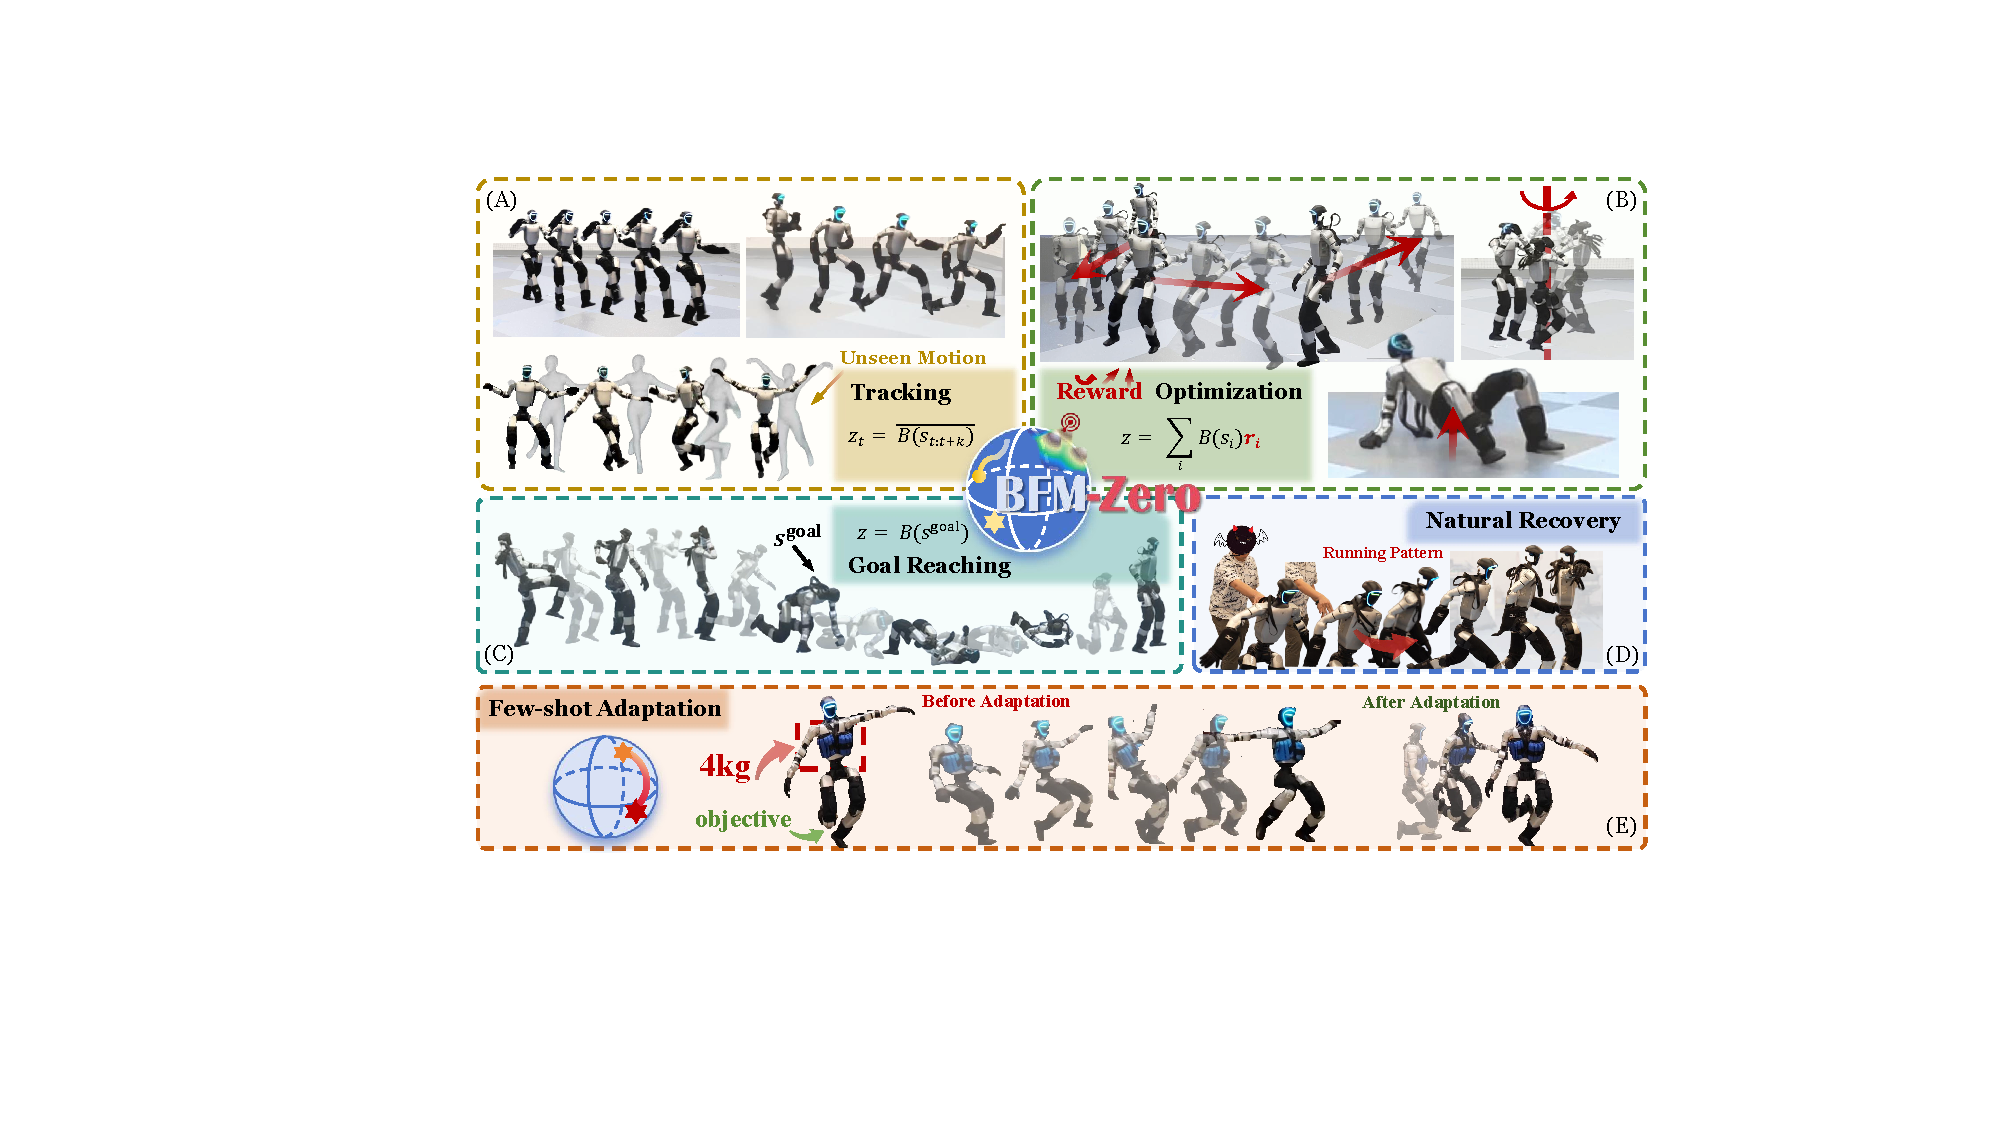
\includegraphics[width=1.0\textwidth]{image/teaser_final.pdf}
    \captionof{figure}{ \small \method{} enables versatile and robust whole-body skills.
    (A-C) Diverse zero-shot inference methods. (D) Natural recovery from large perturbation. (E) Few-shot adaptation.}
    \label{figure_1_teaser}
\end{minipage}
  \tcbline
  \vspace{-1em}
  % Metadata section (after abstract, inside tcolorbox)
  \vskip 0.5cm
  \makeatletter
  \ifdefempty{\metadatalist}{}{\metadatalist\par}
  \makeatother
\end{tcolorbox}

  
\begin{abstract}
Building Behavioral Foundation Models (BFMs) for humanoid robots has the potential to unify diverse control tasks under a single, promptable generalist policy. 
However, existing approaches are either exclusively deployed on simulated humanoid characters, or specialized to specific tasks such as tracking. 
We propose \method{}, a framework that learns an effective shared latent representation that embeds motions, goals, and rewards into a common space, enabling a single policy to be prompted for multiple downstream tasks without retraining. 
% What we unlock in real world
This well-structured latent space in \method{} enables versatile and robust whole-body skills on a Unitree G1 humanoid in the real world, via diverse inference methods, including zero-shot motion tracking, goal reaching, and reward inference, and few-shot optimization-based adaptation.
Unlike prior on-policy reinforcement learning (RL) frameworks, \method{} builds upon recent advancements in unsupervised RL and Forward-Backward (FB) models, which offer an objective-centric, explainable, and smooth latent representation of whole-body motions.
We further extend \method{} with critical reward shaping, domain randomization, and history-dependent asymmetric learning to bridge the sim-to-real gap. 
Those key design choices are quantitatively ablated in simulation.
A first-of-its-kind model, \method{} establishes a step toward scalable, promptable behavioral foundation models for whole-body humanoid control.\\%Videos: \url{http://bfm-zero-anonymous.pages.dev}
\end{abstract}

\vspace{-2mm}
\section{Introduction}
\vspace{-2mm}
% Recent progress has demonstrated impressive capabilities in simulation and on hardware, but current approaches still suffer from three major limitations. First, they remain task-specific: most policies are trained to imitate motion capture clips or solve a single locomotion or manipulation task. Second, they are non-adaptive: once trained, policies cannot be easily fine-tuned or composed for new tasks. Third, they lack a unified and explainable interface for goal specification and behavior composition, making it difficult for human operators to direct the robot or combine learned skills into new behaviors.

% To overcome these limitations, we take inspiration from the success of large language models (LLMs) and vision-language models (VLMs), which pair large-scale pretraining with post-training alignment and test-time adaptation to create versatile general-purpose systems.

% To overcome these limitations, we take inspiration from the success of large language models (LLMs) and vision-language models (VLMs), which pair large-scale pretraining with post-training alignment and test-time adaptation to create versatile general-purpose systems.

% Humanoid is important and WBC is important
Humanoid robots have the potential to transform numerous aspects of our daily lives, from manufacturing and logistics to healthcare and personal assistance. However, realizing this potential requires robots to perform a wide range of tasks in dynamic and unstructured environments. Humanoid whole-body control is a fundamental and challenging problem in robotics, serving as the first step to enable the humanoids to work safely in human environments~\citep{gu2025humanoid}.

% Robotics foundation models
In robotics, foundation models have the potential to unify diverse control objectives under a single policy, allowing robots to adapt to new tasks in a zero-shot\footnote{\emph{Zero-shot} means that, after pre-training, the policy can be directly deployed in the real world without further interacting with either simulated or real environments. In contrast, \emph{few-shot} means the policy needs to interact with the environment to collect new data in few episodes to improve on certain tasks.}way or with efficient post-training. The closest approaches to such paradigms are Vision-Language-Action (VLA) models for robotic manipulations~\citep[e.g.,][]{Ghosh2024octo,pi05,openvla,Zhong2025DexGraspVLA, geminirobotics,grootn1} that learn from human demonstrations (i.e., behavior cloning). However, for humanoid whole-body control, there is a fundamental mismatch that limits direct behavior cloning: unlike manipulation tasks, there are no readily available actuator-level action labels or large-scale teleoperation datasets.
 
 
 % , as the networks are typically optimized for manipulation, where control frequencies can remain relatively low (e.g., issuing a grasp or push command at 5–10 Hz) without compromising task success. By contrast, whole-body humanoid control demands high-frequency actuation (often 50-200 Hz) to maintain balance. 
 
For whole-body humanoid control, most recent advancements follow the sim-to-real pipeline and rely on reinforcement learning (RL) to train policies in simulation before transferring them to hardware~\citep{gu2025humanoid}. Following the success of RL-based motion tracking in physics-based character animation~\citep[e.g.,][]{Luo2024universal, TesslerGNCP24,TirinzoniTFGKXL25zeroshot}, recent works~\citep[e.g.,][]{Zakka2025mujocoplayground,Seo2025fasttd3,Chen2025gmt,liao2025beyondmimic,he2025asap,cheng2024expressive,he2025omnih2o} have shown remarkable results in transferring policies trained in simulation to real robots. However, most of these approaches rely on \emph{on-policy policy gradient} methods (e.g., PPO~\citep{schulman2017proximal}) with \emph{explicit tracking-based rewards} and suffer from major limitations. First, they remain task-specific: most policies are trained to explicitly imitate motion capture clips or solve a single task. Second, they are non-adaptive: once trained, policies cannot be easily fine-tuned or composed for new tasks. Third, they lack a unified and explainable interface for goal specification and behavior composition, making it difficult for human operators to direct the robot or combine learned skills into new behaviors.

%While almost the totality of existing approaches for real-world deployment leverage on-policy training, we 

In this work, we investigate whether \emph{off-policy unsupervised} RL can be a suitable approach to train so-called Behavioral Foundation Models (BFMs) for whole-body control of a humanoid robot, enabling it to solve a wide range of downstream tasks specified by rewards, goals, or demonstrations without retraining. For tasks that require retraining, the BFM should enable efficient post-training. 
% \guanya{todos: add one sentence for efficient post-training}
This conjecture is far from trivial. First, most existing methods with real-world deployment rely on on-policy training (primarily PPO), and there is little evidence that off-policy learning—commonly used in unsupervised RL for training multi-task policies—is well suited to this context. Second, no evidence exists that unsupervised RL algorithms can handle the sim-to-real gap and dynamic disturbances robustly, either during simulation policy training or at real-world inference.

% In particular, we build on the FB-CPR algorithm recently proposed by~\citet{TirinzoniTFGKXL25zeroshot} to control a virtual physics-based humanoid character and we investigate how it can be used to train a BFM for whole-body control of a humanoid robot. 
We develop \method\footnote{\texttt{\textcolor{myred}{\textbf{Zero}}} comes from its zero-shot inference capability via unsupervised RL and it is a first-of-its-kind model.}, an online off-policy unsupervised RL algorithm that leverages motion capture data to regularize the process of learning generalist whole-body control policies towards \emph{human behaviors}. 
We introduce domain randomization to address the sim-to-real gap and train robust policies via asymmetric history-dependent training, leveraging the privileged information available in simulation. Additionally, we incorporate auxiliary rewards to ensure that the learned behaviors adhere to the safety and operational constraints of the physical robot. To the best of our knowledge, the resulting algorithm allows us to train the \emph{first behavioral foundation model} for real humanoids that can be prompted for different tasks (e.g., reward optimization, pose reaching, and motion tracking) without retraining (i.e., in zero-shot). Such a flexible and ready-to-use model, paves the way to fast adaptation, fine-tuning or even high-level planning.
%
We validate our approach in both simulated environments and on a real Unitree G1 humanoid (Fig.~\ref{figure_1_teaser} for examples), demonstrating robust generalization across tasks and conditions, and showing that even when the zero-shot policy is not satisfactory, we can effectively improve it within a few episodes of environment interaction. The discussion of related work is available in \Cref{sec:appendix-related-work}.


% OLD
% In this work, we look into unsupervised reinforcement learning (RL) as a promising paradigm to train so-called \emph{behavioral foundation models} to enable agents to solve a wide range of downstream tasks specified by rewards, goals, or demonstrations without any retraining. In particular, we build on the FB-CPR algorithm recently proposed by~\citet{TirinzoniTFGKXL25zeroshot} to control a virtual physics-based humanoid character and we investigate how it can be used to train a BFM for whole-body control of a humanoid robot. 
% %trained in simulation and transferred zero-shot to a physical robot. Our model is designed to represent behaviors in a latent space shared across states, goals, and rewards, enabling a single policy to be prompted for various tasks (such as motion tracking, goal-reaching, and reward optimization) without retraining. We build on top of the unsupervised RL approach of~\citet{TirinzoniTFGKXL25zeroshot} and address the challenges of sim-to-real transfer. 
% We introduce domain randomization to address the sim-to-real gap and train robust policies via asymmetric history-dependent training to leverage the privileged information available in simulation. Additionally, we incorporate reward regularization to ensure that the learned behaviors adhere to safety and operational constraints of the physical robot. The resulting algorithm allows us to train the \textbf{first behavioral foundation model for the Unitree G1} that is light --the policy can be deployed on the robot's onboard computer-- and general --it can be prompted for different tasks (e.g., reward optimization, pose reaching, and motion tracking) without retraining (i.e., in zero-shot). Such a flexible and ready-to-use model, paves the way to fast adaptation, fine-tuning or even high-level planning, thereby advancing the development of versatile humanoid robots with general-purpose capabilities. 
% %
% We validate our approach in both simulated environments and on a real Unitree G1 robot, demonstrating robust generalization across tasks and conditions, and showing that even when the zero-shot policy is not satisfactory, we can effectively improve it in a matter of few simulated or real episodes.
% \input{section/preliminaries}
\section{BFM-Zero for Humanoid Whole-body Control}\label{sec:training}
\vspace{-2mm}
\begin{figure}[htbp]
    \begin{center}
    \centerline{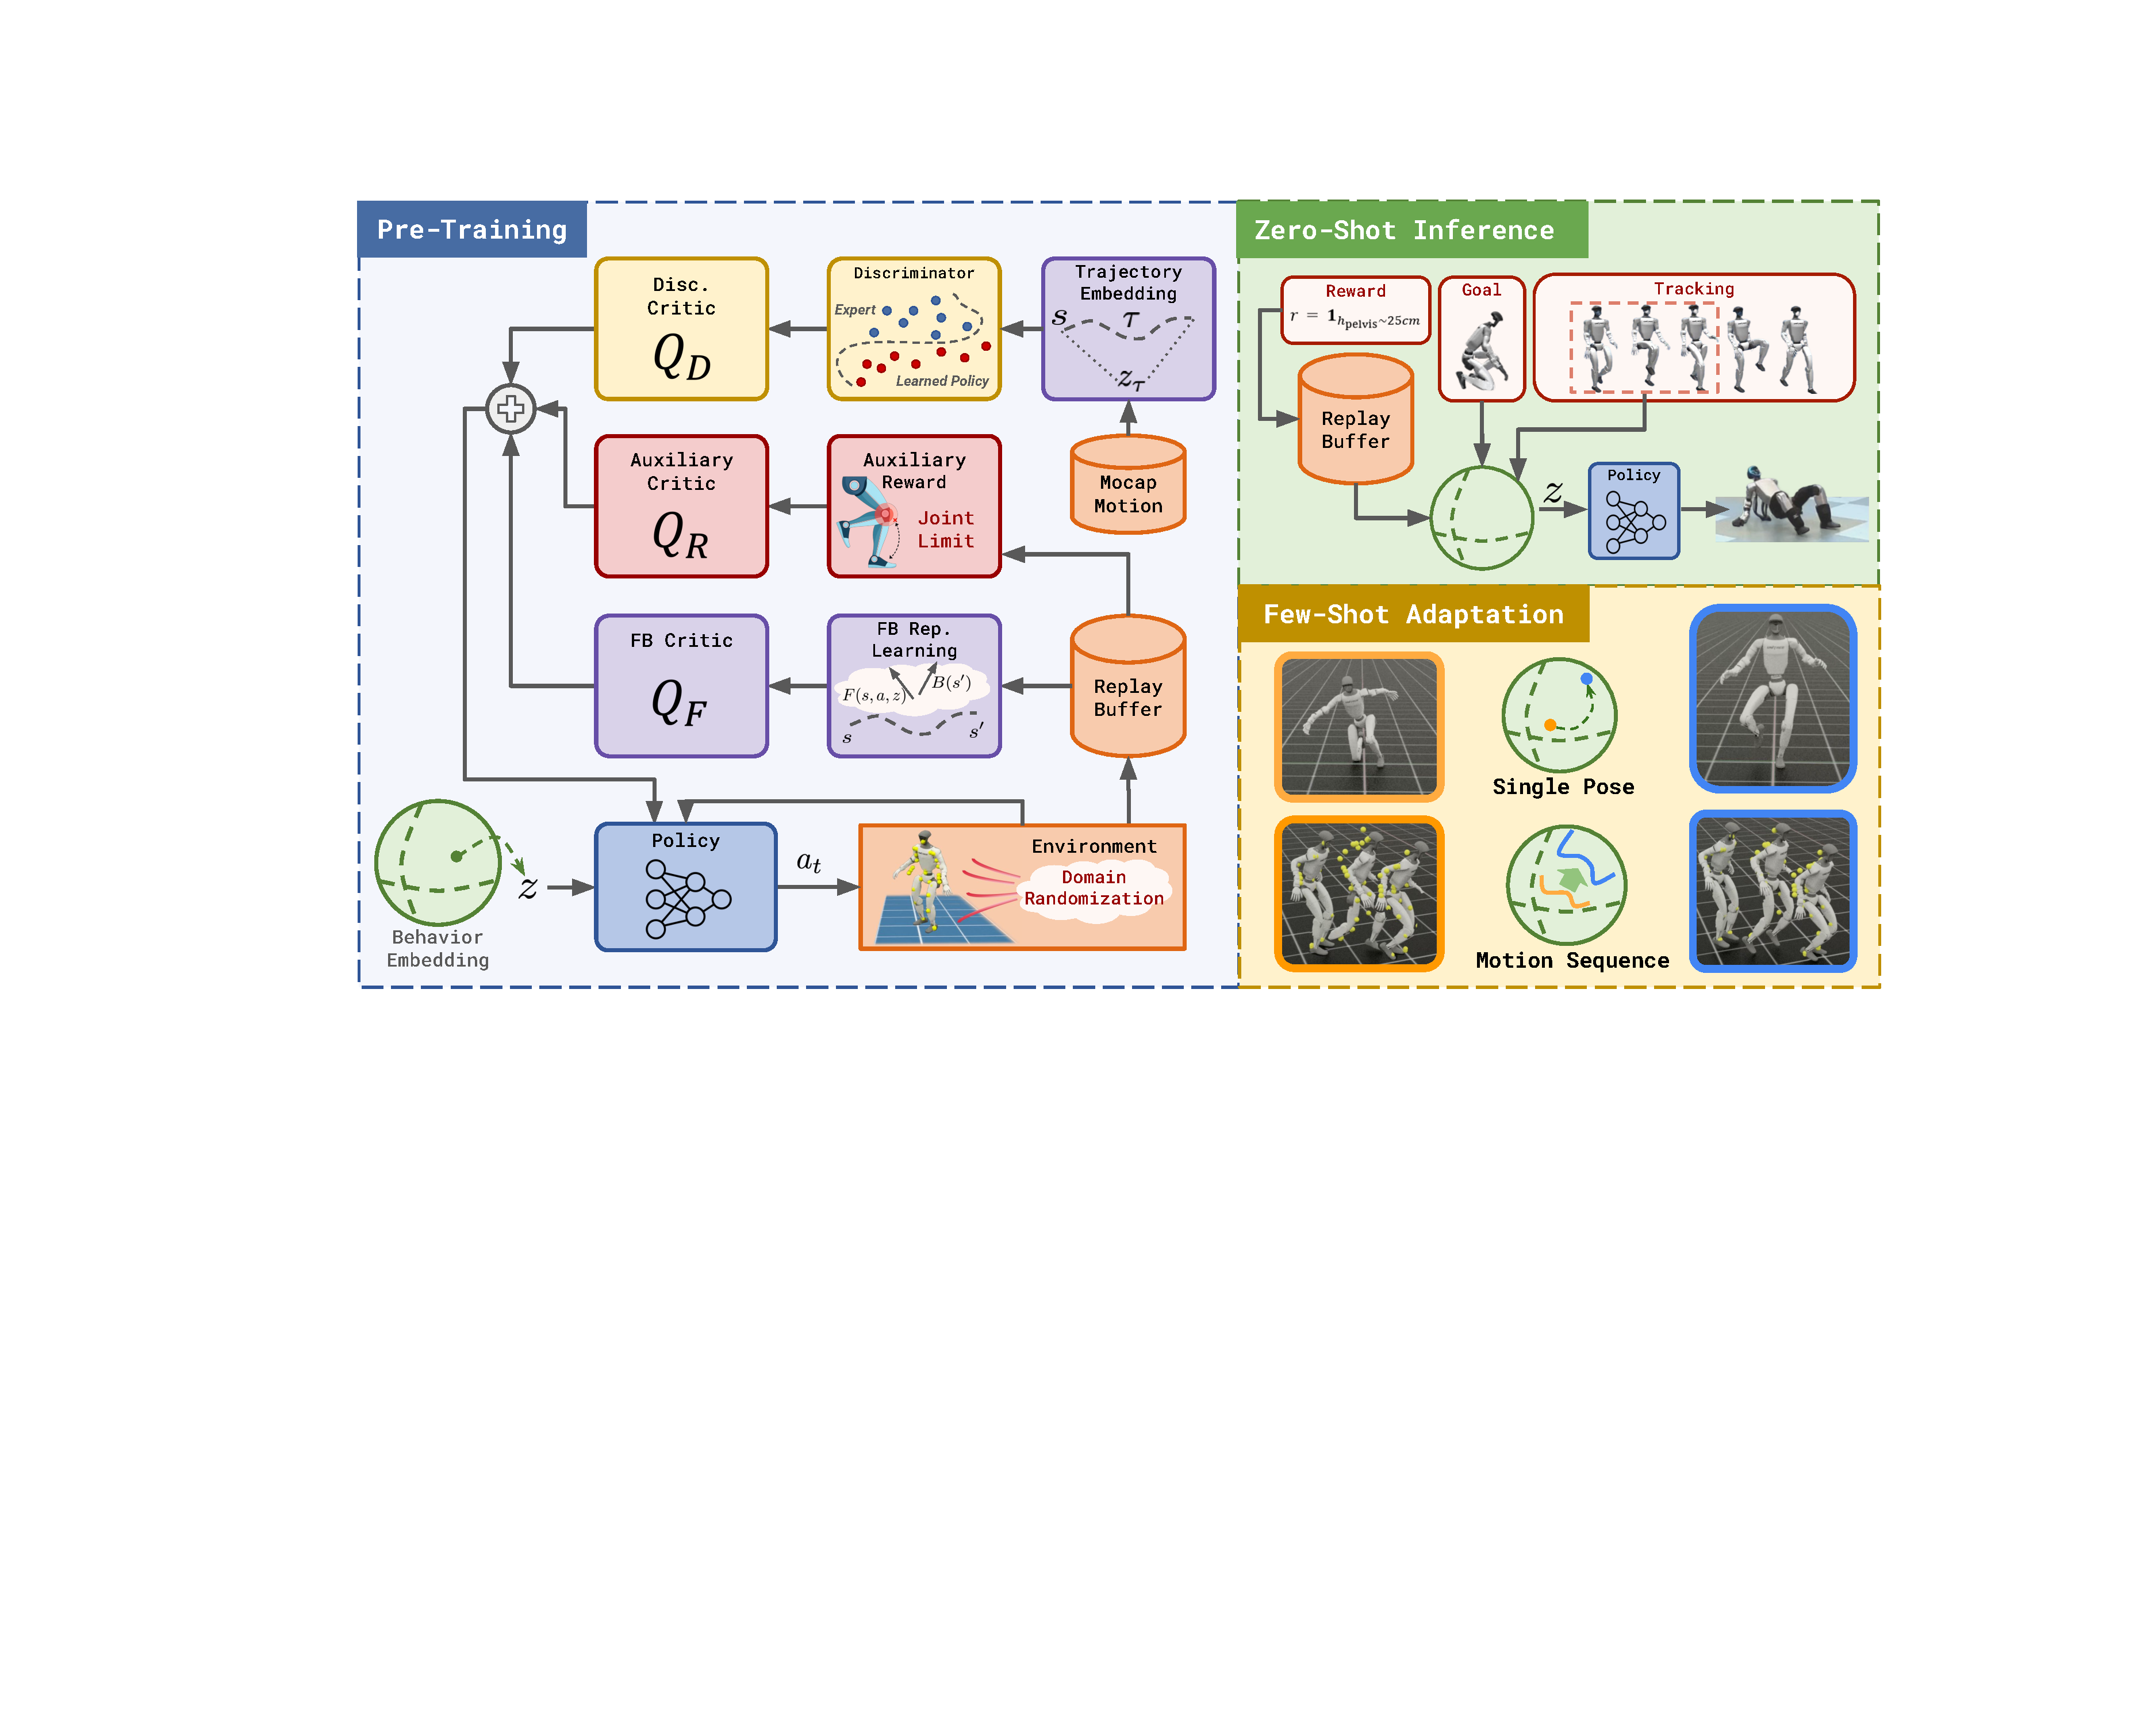
\includegraphics[width=1.0\linewidth]{image/figure_2_pipeline_2col.pdf}}
    \vspace{-0.2cm}
    \caption{\small An overview of the \method{} framework. After the pre-training stage, \method{} forms a latent space that can be used for zero-shot reward optimization, single-frame goal reaching, and tracking. It can also be adapted in a few-shot fashion to reach more challenging poses. }
    \label{fig:bfm.zero}
    \end{center}
\end{figure}

% \begin{figure}[htbp]
%     \centering
%     \includegraphics[width=0.7\textwidth]{image/figure_2_pipeline.pdf}
%     \caption{caption %\anssi{I see the symbols are clarified in the text, but I think different $s$ (proprio, priv, history) should be briefly mentioned in the caption as well.} 
%     %\guanya{I am working on this. Will do: use PDF; replace mocap data with LAFAN photos; use actual simulation image for DR.}
%     }
%     \label{fig:bfm.zero}
% \end{figure}

% \vspace{-.2in}
In this section, we outline the pipeline for training \method{} in simulation and transferring it to real humanoids. Unlike for virtual characters~\citep[e.g.,][]{peng2022ase,tessler2023calm,TirinzoniTFGKXL25zeroshot}, applying unsupervised RL to real humanoids has not yet been attempted. Our \method{} framework consists of an unsupervised pre-training stage, a zero-shot inference procedure, and possibly a fast-adaptation post-training stage (as shown in Fig.~\ref{fig:bfm.zero}). \Cref{sec:prelim} provides an overview of unsupervised RL using the forward-backward representation framework adopted by \method{}. \Cref{sec:pretrain} details \method{} pre-training, whose objective is to learn \emph{a unified latent representation} that embeds tasks (e.g., target motions, rewards, goals) into a shared space $Z \subseteq \mathbb{R}^d$ and \emph{a promptable policy} that conditions on this representation to perform diverse behaviors without task-specific retraining. Then, for downstream tasks during inference (\Cref{sec:inference}), we embed the task into the latent space and use the policy to execute the task in a zero-shot manner. We also show that we can efficiently adapt the zero-shot policy in the latent space $Z$ to improve performance on unseen tasks that are not easily covered by zero-shot inference via sampling-based optimization. % \ale{We don't really adapt the latent space itself, I would rephrase: We also show that starting from the policy obtained via zero-shot inference, we can efficiently adapt it while optimizing \textit{within} the same latent space via MPPI \cite{} and CMA-ES}


% In particular, bridging the sim-to-real gap poses significant challenges, as the dynamics differences between simulation and the real world, partial observation of the robot state, and the heterogeneous levels of hardware capabilities across humanoid platforms make direct transfer difficult. We address these challenges in the following sections and propose \method{}. 



% We address these challenges by combining domain randomization, asymmetric history-dependent training, and reward regularization into the FB-CPR algorithm. %{\color{red} On the other side, models trained for real-world deployment mostly follow a highly parallel on-policy training. We introduce changes to the training of FB-CPR to allow high-parallelization and .}

%We build on top of the recently proposed FB-CPR algorithm~\citep{TirinzoniTFGKXL25zeroshot}, which combines the FB framework reviewed in Sect.~\ref{sec:preliminaries} with a discriminator-based regularization that grounds the unsupervised RL training towards behaviors that are close to those demonstrated in a give set of motions. 
%The resulting model consists of two main components: \textbf{1)} a unified latent representation that embeds tasks (e.g., motions, rewards, goals) into a shared space, and \textbf{2)} a promptable policy that conditions on this representation to execute diverse behaviors without task-specific retraining.



% scaling factors $\beta=5$ and $\alpha_j = 0.25 \frac{\tau_{j,\max}}{k_j^p}$. $\tau_{j,\max}$ represents the maximum allowable joint torque for joint $j$

\textbf{Problem formulation.} We formulate real-world humanoid control as a partially observable Markov decision process (POMDP) defined by the tuple $(S, O, A, P, \gamma)$, where $S$ is the full state space, $O$ is the observation space, $A$ is the action space, $P(s_{t+1}|s_t,a_t)$ is the transition dynamics, and $\gamma \in (0,1)$ is the discount factor. For the 29-degree-of-freedom (DoF) humanoid, the action $a\in A \subset \mathbb{R}^{29}$ contains the proportional derivative (PD) controller targets for all DoFs. The privileged information  ($s \in \mathbb{R}^{463}$) consists of root height, body pose, body rotation, and linear and angular velocities. The observable state $o_t = \{q_t - \bar{q}, \dot{q}_t, \omega^{\mathrm{root}}_t / 4, g_t\} \in \mathbb{R}^{64}$ is defined as joint position $q_t \in \mathbb{R}^{29}$ normalized w.r.t.\ the nominal position $\bar{q}$, joint velocity $\dot{q}_t \in \mathbb{R}^{29}$, root angular velocity $\omega^{\mathrm{root}}_t \in\mathbb{R}^3$ and root projected gravity $g_t \in\mathbb{R}^3$. We denote by $o_{t,H} = \{o_{t-H}, a_{t-H},  \ldots, o_t\}\in \mathbb{R}^{93\cdot H + 64}$ the observable history composed by proprioceptive state and action. 
All the components of the states (except root height) are normalized w.r.t.\ the current facing direction and root position.
At pre-trainig, we assume that the agent has  access to a dataset of unlabeled motions $\mathcal{M} = \{ \tau\}$, which contains observation and privileged states trajectories \textit{i.e} $\tau = (o_1, s_1, \ldots, o_{l(\tau)}, s_{l(\tau)})$.  
% we use a proportional derivative (PD) controller at each joint, resulting in an action space $a \in \mathbb{R}^{29}$.

\subsection{Unsupervised RL with Forward-Backward Representations}
\label{sec:prelim}
\vspace{-2mm}
% following, we define the torque at time $t$ for joint $j$ to be
% \[
% \tau_{j,t} = k^p_j (\hat{q}_{j,t} - q_{j,t}) - k_j^d\; \dot{q}_{j,t}, \quad \hat{q}_{j,t} = \bar{q}_j + \alpha_j \beta a_{j,t}
% \]
% where $k^p_j$ and $k^d_j$ are stiffness and damping gains, $q_{j,t}$ is the robot joint state and $\dot{q}_{j,t}$ is the robot joint velocity. The joint setpoint $\hat{q}_{j,t}$ is computed based on the nominal joint configuration $\bar{q}_j$, the policy action $a_{j,t} \in [-1,1]$, and scaling factors $\beta=5$ and $\alpha_j = 0.25 \frac{\tau_{j,\max}}{k_j^p}$. $\tau_{j,\max}$ represents the maximum allowable joint torque for joint $j$.



% \textbf{Observation.} We denote by $s$ the full state (a.k.a.\ privileged information) available in simulation (but not in the real world) and by $o$ the observable state of the robot in the real world (a.k.a. proprioceptive). The privileged information  ($s \in \mathbb{R}^{463}$) consists of root height, body pose, body rotation, and linear and angular velocities. The observable state $o_t = \{q_t - \bar{q}, \dot{q}_t, \omega^{\mathrm{root}}_t / 4, g_t\} \in \mathbb{R}^{64}$ is defined as joint position $q_t \in \mathbb{R}^{29}$ $\bar{q}$, joint velocity $\dot{q}_t \in \mathbb{R}^{29}$, root angular velocity $\omega^{\mathrm{root}}_t \in\mathbb{R}^3$ and root projected gravity $g_t \in\mathbb{R}^3$. We denote by $o_{t,H} = \{s^p_{t-H}, a_{t-H},  \ldots, s^p_t\}\in \mathbb{R}^{93\cdot H + 64}$ the observable history composed by proprioceptive state and action. All the components of the states (except root height) are normalized w.r.t.\ the current facing direction and root position~\citep{WonGH22,Luo2023phc,TirinzoniTFGKXL25zeroshot}.

% builds on top of the recently proposed FB-CPR algorithm~\citep{TirinzoniTFGKXL25zeroshot},

During the pretraining phase, \method{} learns a compact representation of the environment by observing online reward-free interactions in the simulator and leveraging an offline dataset of unlabeled behaviors, resulting in a model that can be prompted to tackle a wide range of downstream tasks (e.g., tracking or reward maximization) in a zero-shot manner. To achieve this, we build on top of the recent FB-CPR algorithm~\citep{TirinzoniTFGKXL25zeroshot} which combines the Forward-Backward (FB) method for zero-shot RL \citep{Touati21fb} with online training and policy regularization on motion-capture data. This method falls in the broader category of unsupervised RL based on successor features~\citep[e.g.,][]{Touati21fb,touatizerorl,Pirotta24fastimitation,park2024foundation,agarwal2024proto}, which involves three components: (i) a latent task feature $\phi: S \rightarrow \mathbb{R}^d$ that embeds observation $s \in S$ into a $d$-dimensional vector, (ii) a policy $\pi_z: S\rightarrow A$  conditioned on a latent vector $z \in \mathbb{R}^d$, and (iii) latent-conditioned successor features~\citep{barreto2017successor} $F_z$ that encode the expected discounted sum of latent task features under the corresponding policy $\pi_z$, i.e, $F_z \simeq \mathbb{E}[\sum_{t} \gamma^t \phi(s_t)\mid \pi_z ]$. We now explain how FB-CPR trains those components.


% The representation $\phi$ defines a latent task space by inducing a family of linear reward functions of the form, i.e., $r_z(s) = \phi(s)^\top z$, which are used as \textit{unsupervised signal} to train the policy family. In particular, each policy $\pi_z$ is optimized to maximize $\mathbb{E}[ \sum_t \gamma^t r_z(s_t) \mid \pi_z]$, which can be equivalently expressed as $\mathbb{E}[ \sum_t \gamma^t \phi(s_t)^\top z \mid \pi_z] \simeq F_z^\top z$. Intuitively, $z \in Z$ defines a \emph{task-centric} latent space associated with the task feature $\phi$, where for each $z$, the corresponding $\pi_z$ optimizes the linear combination of $\phi$, $r_z=\phi^\top z$. As shown in \Cref{sec:latent}, the $Z$ space learned by \method{} is smooth, explainable, and semantically meaningful and enables both zero-shot inference and few-shot adaptation. Importantly, in contrast to standard RL approaches, $r_z$ is not given (e.g., motion tracking) but learned. Therefore, it can represent a wide range of tasks.

\textbf{FB representations and FB-CPR.} Among the different unsupervised RL approaches, forward-backward (FB) representations provide a principled unsupervised training objective for jointly learning latent task representations and their associated successor features. At a high level, FB learns a finite-rank approximation of long-term policy dynamics, where $\backward$ captures the low-frequency features that best summarize the long-range temporal dependencies between states.  Formally, given a training state distribution $\rho$, the FB framework learns two mappings: a forward mapping $\forward: S \times A \times \mathbb{R}^d \rightarrow \mathbb{R}^d$ and a backward mapping $\backward: S \rightarrow \mathbb{R}^d$ such that the long-term transition dynamics induced by the policy $\pi_z$ decompose as:
\begin{equation}~\label{eq:fb_def}
    M^{\pi_z}(\mathrm{d}s' \mid s, a) \simeq \forward(s, a, z)^\top \backward(s') \rho(\mathrm{d}s')
\end{equation}
where for any region $X \subset S$ of the state space, $M^{\pi_z}(s' \in X \mid s, a) := \sum_{t} \gamma^t \mathrm{Pr}(s_t \in X \mid s, a, \pi_z)$ denotes the discounted visitation probabilities of reaching $X$ under the policy $\pi_z$, starting from the state-action pair $(s, a)$. Eq.~\ref{eq:fb_def} implies that $\forward$ is the successor features of $\phi(s) := ( \mathbb{E}_{\rho}[\backward(s) \backward(s)^\top])^{-1} \backward(s)$~\citep{touatizerorl}.
The learned representation $\phi$ defines a latent task space by inducing a family of linear reward functions of the form, i.e., $r_z(s) = \phi(s)^\top z$, In particular, each policy $\pi_z$ is optimized to maximize $\mathbb{E}_{\rho}[\sum_t \gamma^t \phi(s_t)^\top z \mid \pi_z] = \forward(s,a,z)^\top z$, i.e., $\forward(s,a,z)^\top z$ is a Q-value function of $\pi_z$ with reward $r=\phi^\top z$. Intuitively, $z \in Z$ defines a \emph{task-centric} latent space associated with the task feature $\phi$, where for each $z$, the corresponding $\pi_z$ optimizes the linear combination of $\phi$, $r_z=\phi^\top z$. As shown in \Cref{sec:latent}, the $Z$ space learned by \method{} is smooth and semantic, and it enables both zero-shot inference and few-shot adaptation. Importantly, in contrast to standard RL approaches, the set of reward functions of interest $\{r_z\}$ is not given (e.g., motion tracking) but learned, and it can represent a wide range of tasks. 
%
FB-CPR~\citep{TirinzoniTFGKXL25zeroshot} extends the general FB framework by introducing a latent-conditioned discriminator to regularize the unsupervised learning process to produce policies that are close to a set of demonstrated behaviors in a motion dataset $\mathcal{M}$. Furthermore, while FB algorithm is offline, FB-CPR is trained fully online and off-policy and does not require a full-coverage offline dataset.
% This means that for each $z$, $\mathbb{E}_{\rho}[\sum_t \gamma^t \phi(s_t)^\top z \mid \pi_z] = \forward(s,a,z)^\top z$, i.e., $\forward(s,a,z)^\top z$ is a Q-value function of $\pi_z$ with reward $r=\phi^\top z$. 
%
% \paragraph{Zero-shot generalization to new tasks}
% Given an \emph{arbitrary} reward function $r(s)$, the corresponding Q function of $\pi_z$ can be formulated as 

% \begin{align}
%     Q_r^{\pi_z}(s,a) &= \mathbb{E}[\sum_t \gamma^t r(s_t)] = \int_{s'} M^{\pi_z}(\mathrm{d}s' \mid s, a) r(s') \\ 
%     &\simeq \int_{s'} \forward(s,a,z)^\top \backward(s') r(s') \rho(\mathrm{d}s')=
%     \forward(s,a,z)^\top \int_{s'} \backward(s') r(s') \rho(\mathrm{d}s')
% \end{align}

% Since $\forward(s,a,z)^\top z$ is the Q function of $\pi_z$, we have $z_r = \sum_{s} \backward(s) r(s)$. In other words, once the FB representations are learned, for any new tasks with reward $r$, the corresponding latent vector $z_r$ and the policy $\pi_{z_r}$ can be efficiently computed in a \emph{zero-shot} way. For example, for a goal-reaching task where $r(s)=\mathbbm{1}(s=s_g)$, we have $z_r=B(s_g)$. 

% \begin{align}
% Q_r^\pi(s,a) = E[\sum_{t}\gamma^t r_{t+1}] = \sum_{s'} M^\pi(s'|s,a) r(s') =
% \sum_{s'} F^\pi(s,a) B(s') r(s') =
% F^\pi(s,a) \sum_{s'} B(s') r(s') = 
% F^\pi(s,a) z_r
% \end{align}
%
% \paragraph{Zero-shot reward inference} Given a new reward function $r(s)$, the goal of reward inference is to find a latent vector $z \in Z$ such that 
% \begin{equation}
%     r(s) \approx \phi(s)^\top z = \backward(s)^\top (\mathbb{E}_{\rho}[\backward(s) \backward(s)^\top])^{-1} z 
% \end{equation}
%
% Example for goal reaching: When $z = B(s_i)$, the corresponding reward is 
% \begin{equation}
%     \phi(s)^\top \backward(s_i) = \backward(s)^\top (\sum_{i=1}^N \frac{1}{N} \backward(s_i) \backward(s_i)^\top)^{-1} \backward (s_i)
% \end{equation}
%
% At a high level, FB learns a finite-rank approximation of long-term policy dynamics, where $\backward$ captures the low-frequency features that best summarize the long-range temporal dependencies between states. 
% In \Cref{sec:pretrain}, we train FB within an off-policy actor-critic scheme, where the forward and backward mappings are trained using a temporal-difference loss~\citep{blier2021learning}, while the policies are updated via deterministic policy gradients.  










% ================== Current Version ==================


% At the pretraining stage, \method{} aims to learn an interpretable latent space that can be zero-shot applied to tasks like tracking and reward-maximizing, as well as being efficiently adapted to challenging cases. 
% To achieve this, we adopt a TD-based actor-critic algorithm for unsupervised RL ~\citep[e.g.,][]{Touati21fb,touatizerorl,Pirotta24fastimitation,TirinzoniTFGKXL25zeroshot,park2024foundation,agarwal2024proto,jajoo2025regularized} and learns a forward mapping $\forward$, a backward mapping $\backward$, a policy (actor) $\actor$, and three critics to optimize the latent space: a forward-backward $\fbcritic$ for learning the latent representation, a discriminator $\disccritic$ for learning human-like behavior, and an auxiliary critic $\auxcritic$ for regulating the learned policy behaviors for sim-to-real transfer. \yitang{I think we can make this part more intuitive} 


% Formally, \method{}  builds on the notion of successor features~\citep[e.g.,][]{barreto2017successor} and first learns a forward $\forward$ and backward mapping $\backward$ to approximate a low-rank decomposition of the dynamics of the learning policies. Given a class of reward functions, $R_\phi = \{r(s) = \phi(s)^\top z_r\}$, the Q-values for any reward $r(s) = \phi(s)^\top z_r$ can be written as
% \begin{equation}
%     Q^\pi_r(s,a) = \int_{s' \in S} M^\pi(\mathrm{d}s' \mid s, a) \phi(s')^\top z_r 
% % =\mathbb{E}_{s^+\sim M^\pi(\cdot|s,a)}\big[\phi(s^+)\big]^\top z_r 
% =  \forward ^\pi(s,a)^\top z_r,
% \end{equation}

% where, $\forall \mathcal{X} \subseteq S$, $M^\pi(\mathcal{X} |s,a) = \sum_{t=0}^\infty \gamma^t \mathrm{Pr}(s_t \in \mathcal{X}| s,a,\pi)$ is the successor measure, $\forward^\pi(s,a)$ is the successor features of $\pi$, i.e., the average of the features $\phi$ associated to the states traversed by the policy. $s'$ refers to a possible future state. 
% The Forward-Backward (FB) model proposed by~\citep{Touati21fb} et of parametrized policies $\{\pi_z(s)\}_{z \in Z}$ with $z \in \mathbb{R}^d$ that are trained to be optimal for all rewards $R_\phi$, i.e.,
% \begin{equation}\label{eq:policy_opt_successor_feat}
% \pi_z(s) \approx \argmax_a \forward(s,a;z)^\top z,
% \end{equation}
% where $\forward(s,a;z)^\top z \approx Q^\star_r(s,a) = \max_{\pi}Q^\pi_r(s,a)$ and $r(s) = \phi(s)^\top z$, where the reward features $\phi$ are learned jointly with $\forward$ and the policies $\pi_z$. Combining the forward $\forward$ and $\backward$ mapping, we approximate the dynamics of the policy: 
% \begin{equation}\label{eq:fb_approx}
% F(s,a;z)^\top B(s') \approx M^{\pi_z}(ds'|s,a)
% \end{equation}
% that when combined with Eq.~\ref{eq:policy_opt_successor_feat} leads to $\phi(s) = \mathbb{E}_s[\backward(s)\backward(s)^\top]^{-1} \backward(s)$. 
% Intuitively, the FB algorithm implements an \textit{inductive bias} to jointly train policies and rewards, where the policies are optimal for the rewards, and the rewards can be expressed as linear functions of features $B$ that capture the ``low-frequency'' dynamics of the policies.  In practice, an FB model is fully \emph{unsupervised} since solving Eq.~\ref{eq:fb_approx} and Eq.~\ref{eq:policy_opt_successor_feat} does not require any reward signal during training. 
% The Forward-Backward representations with Conditional Policy Regularization~\citep[FB-CPR]{TirinzoniTFGKXL25zeroshot} extends the general FB framework by introducing a latent-conditioned discriminator to regularize the unsupervised learning process to produce policies that are close to a set of demonstrated behaviors in a motion dataset.

% To optimize the forward $\forward$ and $\backward$ mappings, we learn an FB critic $\fbcritic$, which is similar to the standard Q-function in successor feature learning as $\forward(s,a;z)^\top z \approx Q^\star_r(s,a) = \argmax_{\pi}Q^\pi_r(s,a)$.  We also learn an auxiliary critic $\auxcritic$  that imposes safety and physical feasibility constraints by incorporating penalty rewards (e.g., joint limits, slippage, self-collisions). This ensures that the learned behaviors remain transferable to real humanoid hardware. Finally, we employ the discriminator critic $\disccritic$ that grounds the unsupervised training toward human-like behaviors by assigning rewards based on a latent-conditioned discriminator. This prevents the policy from drifting to unrealistic motions and aligns it with the distribution of demonstrated trajectories. At the pre-training stage, we use a dataset of unlabeled motions $\mathcal{M} = \{\tau\}$, where each motion $\tau$ is a trajectory of observations $\tau = (x_1, x_2, \ldots, x_T)$ from the retargeted LAFAN1 dataset~\citep{HarveyYNP20lafan1}. 

\subsection{BFM-Zero Pre-training for Humanoid Control}
\label{sec:pretrain}
\vspace{-3mm}
Before proceeding with the description of implementation details, we identify several design choices that are crucial for achieving sim-to-real transfer in unsupervised RL.


\textit{A) Asymmetric Training.} To bridge the gap between simulation (full state) and real robot (partial observability), we train the policy on observation history $o_{t,H}$, while critics have access to privileged information $(o_{t,H}, s_t)$. This setup improves policy robustness under limited sensing while leveraging privileged critics to provide accurate value estimates. Using history narrows the information gap between proprioceptive actors and privileged critics and improves adaptability under domain randomization.


\textit{B) Scaling up to Massively Parallel Environments.} Inspired by recent work on large-batch off-policy RL~\citep{Seo2025fasttd3}, we scale training across thousands of environments with large replay buffers and high update-to-data (UTD) ratios. This enables efficient unsupervised training of a diverse family of policies while retaining stability, a crucial step for scaling humanoid pretraining.


\textit{C) Domain Randomization (DR).} To enhance robustness and adaptability, we randomize key physical parameters (link masses, friction coefficients, joint offsets, torso center-of-mass) and apply perturbations and sensor noise. This prevents overfitting to simulation dynamics and ensures that policies remain stable when deployed on real hardware (see  Fig.~\ref{fig:dr_and_reg} in Appendix).

\textit{D) Reward Regularization.} In robotics~\citep[e.g.,][]{he2025asap,Zakka2025mujocoplayground}, it is common to incorporate reward regularization techniques to avoid undesirable behaviors. For example, reaching the limit of the joint may lead to highly nonlinear behaviors that are difficult to model in simulation or even damage the robot's hardware.
%Please refer to Figure~\ref{fig:dr_and_reg} for a list of the penalty rewards used in our implementation and their weights.

%
% With these in mind, we can now detail the components of \method{}. \textbf{1)} A latent task space $Z \subseteq \mathbb{R}^d$ (here the unit hypersphere of radius $\sqrt{d}$); \textbf{2)} a \textit{privileged} backward embedding $\boldsymbol{B}: O \times S \to Z$ mapping states to latent task; \textbf{3)} a policy-conditional, \emph{history-based}, \emph{privileged} forward embedding $\boldsymbol{F}: (O \times A)^H \times S \times A \times Z \to \mathbb{R}^d$ that provides an estimate of the successor features under the learned policies  \textbf{4)} a promptable \emph{history-based} conditional policy $\pi: (O \times A)^H \times  Z \to A$; \textbf{5)} a \textit{privileged} latent-conditional discriminator $\boldsymbol{D}: O \times S \times Z \to \mathbb{R}$ that provides a training signal to steer the learned behaviors toward capturing behaviors represented in the motion dataset and finally the associated \emph{history-based}, \emph{privileged} critic $\disccritic: (O \times A)^H \times S \times A \times Z \rightarrow \mathbb{R}$ trained for each policy on top of the discriminator reward. We train \method{} within an off-policy actor-critic scheme, where the forward and backward mappings are trained using a temporal-difference loss~\citep{blier2021learning}, while the policies are updated via deterministic policy gradients.  


% \textit{D) Reward Regularization.} In robotics~\citep[e.g.][]{he2025asap,Zakka2025mujocoplayground}, it is common to incorporate reward regularization techniques to avoid undesirable behaviors. For example, reaching the limit of the joint may lead to highly unlinear behaviors that are difficult to model in simulation or even  to damage the robot's hardware. To address these hard constraints, we introduce an \emph{auxiliary critic} $\auxcritic(o_{t,H}, s_t, a_t,z)$ trained using a combination of penalty rewards (e.g., joint limits, feet slip, action rate, etc.) to ensure that the learned behaviors adhere to safety and operational constraints of the physical robot. This is used as an additional regularization in the policy training loss, leading to
% \[
% \ell(\pi) = - \mathbb{E}_{x \sim \mathcal{D}_{\mathrm{online}}, z\sim \nu, a \sim \pi_z(\cdot| s)} \big[ \fbcritic(x,z) + \alpha_D \disccritic(x,z)  + \alpha_R \auxcritic(x,z) \big],
% \]
% where $x=(o_{t,H}, s_t, a_t)$. Please refer to Figure~\ref{fig:dr_and_reg} for a list of the penalty rewards used in our implementation and their weights.

We train \method{} within an off-policy actor-critic scheme.
The policy-conditional, \emph{history-based}, \emph{privileged} forward map $\forward$ and \textit{privileged} backward map $\backward$ are trained to minimize the
temporal difference loss derived from the  Bellman equation for successor measures~\citep{Touati21fb}. Let $\mathcal{D}$ the replay buffer of online interactions with the simulator and $\nu$ is an arbitrary distribution over $Z$, we consider the following FB objective:
% \begin{align}\label{eq:fb.loss}
%     \mathcal{L}(F,B) &= \mathbb{E}_{\substack{z\sim\nu, (x,a,x') \sim \mathcal{D},\\ x^{+}\sim\mathcal{D}, a'\sim\pi_{z}(x')}} \Big[ \big( F(x,a,z)^\top B(x^+) - \gamma \overline{F}(x',a', z)^\top \overline{B}(x^+)\big)^2 \Big] \\
%     &\quad - 2 \mathbb{E}_{z\sim\nu, (x,a,y)\sim \rho}\big[ F(x,a,z)^\top B(y)\big],\nonumber
% \end{align}
% where $\nu$ is an arbitrary distribution over $Z$.
\begin{align*}\label{eq:fb.loss}
    \mathcal{L}(\boldsymbol{F},\boldsymbol{B}) &= \mathbb{E} \Big[ \big( \boldsymbol{F}(o_{t, H},s_t, a_t, z)^\top \boldsymbol{B}(o^{+}, s^{+}) - \gamma \overline{\boldsymbol{F}}(o_{t+1, H},s_{t+1}, a_{t+1}, z)^\top \overline{\boldsymbol{B}}(o^{+}, s^{+})\big)^2 \Big] \\
    &\quad - 2 \mathbb{E}\big[ \boldsymbol{F}(o_{t, H},s_t, a_t, z)^\top \boldsymbol{B}(o_{t+1}, s_{t+1}) \big],\nonumber
    % & \text{where } z\sim \nu, (o_{t, H},s_t, a_t, o_{t+1, H},s_{t+1}, s_{t+1}, a_{t+1}) \sim \mathcal{D}_{\mathrm{online}} \text{ and } (o^{+}, s^{+}) \sim \mathcal{D}_{\mathrm{online}} \nonumber
\end{align*}
where $z\sim \nu, (o_{t, H},s_t, a_t, o_{t+1, H},s_{t+1}) \sim \mathcal{D}$, $a_{t+1} = \pi(o_{t+1, H}, z)$ and $(o^{+}, s^{+}) \sim \mathcal{D}$. $\overline{\boldsymbol{F}}$ and $\overline{\boldsymbol{B}}$ denote the stop-gradient operator.


%
% we learn an FB critic $\fbcritic$, which is similar to the standard Q-function in successor feature learning as $\forward(s,a;z)^\top z \approx Q^\star_r(s,a) = \argmax_{\pi}Q^\pi_r(s,a)$.  The backward mapping $\boldsymbol{B}$ acts as a task encoder as well as a policy encoder. The forward map $\boldsymbol{F}$
% We also learn an auxiliary critic $\auxcritic$  that imposes safety and physical feasibility constraints by incorporating $N_{\mathrm{aux}}$ penalty rewards (e.g., joint limits, slippage, self-collisions). This ensures that the learned behaviors remain transferable to real humanoid hardware. 
The auxiliary \emph{history-based}, \emph{privileged} critic $\auxcritic$ that imposes safety and physical feasibility constraints by incorporating $N_{\mathrm{aux}}$ penalty rewards is learned with a standard Bellman residual loss:
\begin{small}
\[
\mathcal{L}(\boldsymbol{Q_R})= \mathbb{E}_{\substack{(o_{t, H}, s_t, a_t, s_{t+1}) \sim \mathcal{D}\\ z\sim\nu, a_{t+1}=\pi(o_{t+1, H}, z)}} \left[ \Big(\boldsymbol{Q_R}(o_{t, H}, s_t, a_t, z) - \sum_{k=1}^{N_{\mathrm{aux}}} r_k(s_t) - \gamma \overline{\boldsymbol{Q_R}}(o_{t+1, H},s_{t+1}, a_{t+1}, z)\Big)^2\right].
\]
\end{small}
Finally, we employ the \emph{history-based}, \emph{privileged} discriminator critic $\disccritic$ that grounds the unsupervised training toward human-like behaviors by assigning rewards based on a latent-conditioned discriminator. This acts both as a style regularization as well as a bias in the online exploration process. 
%This prevents the policy from drifting to unrealistic motions and aligns it with the distribution of demonstrated trajectories.
As in~\citep{TirinzoniTFGKXL25zeroshot}, we employ a variational representation of the Jensen-Shannon divergence and train the discriminator $\boldsymbol{D}$ with a GAN-style objective:
\begin{align*}\label{eq:disc-loss}
    \mathcal{L}(\boldsymbol{D}) = 
    -\mathbb{E}_{\substack{\tau \sim \mathcal{M}, (o, s) \sim \tau }} \left[ \log(\boldsymbol{D}(o, s, z_\tau))\right] -\mathbb{E}_{\substack{(o, s, z) \sim \mathcal{\boldsymbol{D}}}} \left[\log(1 - \boldsymbol{D}(o, s, z))\right].
\end{align*}
where $z_\tau=\frac{1}{l(\tau)} \sum_{(o,s) \in \tau} \boldsymbol{B}(o,s)$ is a zero-shot imitation embedding of the motion $\tau$. We can then fit a \emph{style} critic $\disccritic$ with a Bellman residual loss similar to the auxiliary critic with a reward $r_d(o_t,s_t,z)=\frac{\boldsymbol{D}(o_t,s_t,z)}{1-\boldsymbol{D}(o_t,s_t,z)}$.
% \[
% \mathcal{L}(\boldsymbol{Q_D}) = \mathbb{E} \left[ \Big(\boldsymbol{Q_D}(o_{t, H}, s_t, a_t, z) - \frac{\boldsymbol{D}(o_t,s_t,z)}{1-\boldsymbol{D}(o_t,s_t,z)}  - \gamma \overline{\boldsymbol{Q_D}}(o_{t+1, H}, s_{t+1}, a_{t+1}, z)\Big)^2\right]
% \]
Bringing together these critiques results in the final actor loss. % for \method{},
\begin{equation*}\label{eq:actor_loss}
    \mathcal{L}(\pi) = - \mathbb{E}_{\substack{(o_{t, H},s_t) \sim \mathcal{D}\\
    a_{t} = \pi(o_{t, H}, z), z \sim \nu, }} \Big[ \boldsymbol{F}(o_{t, H}, s_t,a_t, z)^\top z + \lambda_D \boldsymbol{Q_D}(o_{t, H}, s_t,a_t, z) + \lambda_R \boldsymbol{Q_R}(o_{t, H}, s_t,a_t, z)\Big].
\end{equation*}
% At the pre-training stage, we use a dataset of unlabeled motions $\mathcal{M} = \{\tau\}$, where each motion $\tau$ is a trajectory of observations $\tau = (x_1, x_2, \ldots, x_T)$ from the retargeted LAFAN1 dataset~\citep{HarveyYNP20lafan1}. T
% The overall structure of \method{} pre-training is summarized in Fig.~\ref{fig:bfm.zero}. %We refer the reader to Appendix~\ref{} for details about the training procedure.



%
% \ale{Add details of what is in $s^p$ and what is in $s^v$?} More precisely, the model inputs are as follows:
% \begin{itemize}
%     \item The critics $F$, $Q_D$, and $Q_R$ take as input the full state $(s^p_t, s^o_t)$ and the last action $a_{t-1}$ over a $H$-step window. Let $x_t = (s^p_t, s^o_t, a_{t-1})$ be the extended state, then input of the critics is $s_{\mathrm{critic},t} = (x_t, x_{t-1}, \ldots, x_{t-H+1})$.
%     \item The backward map $B$ and the discriminator $D$ receives in input the full state, i.e., $s_t = (s^p_t, s^o_t)$. We don't use actions since they are not available in the unlabeled dataset of behaviors. We don't use history for these models.
%     \item The policy $\pi$ is provided with the proprioceptive state and the last action, i.e., $y_t = (s^p_t, a_{t-1})$, but no privileged state. Similarly to the critic we use a $H$-step window leading to $s_{\mathrm{policy},t} = (y_t, y_{t-1}, \ldots, y_{t-H+1})$
% \end{itemize}
%


% \begin{table}[t]
% \begin{wraptable}{l}{.4\textwidth}
%     \resizebox{.4\textwidth}{!}{%
%     \begin{tabular}{|c|c|}
%         \hline 
%         % Parameter & Range \\
%         % \hline\hline
%         \multicolumn{2}{|c|}{Dynamics Randomization} \\
%         \hline
%         COM \emph{displacement} [m] & $\mathcal{U}([-0.02, 0.02])$\\
%         Link mass \emph{multiplier} & $\mathcal{U}([0.95, 1.05])$\\
%         Friction & $\mathcal{U}([-0.5, 1.25])$\\
%         \makecell{Nominal joint position\\ \emph{displacement} [m]} & $\mathcal{U}([-0.02, 0.02])$\\
%         External perturbation [m/s] & $\mathcal{U}([0, 0.5])$\\
%         \hline
%         \hline
%         \multicolumn{2}{|c|}{Additive Observation Noise} \\
%         % \hline
%         % Parameter & Range\\
%         \hline
%         $q_t - \bar{q}$ & $\mathcal{U}([-0.01, 0.01])$\\
%         $\dot{q}_t$ & $\mathcal{U}([-0.5,0.5])$\\
%         $\mathrm{grav}_t$ & $\mathcal{U}([-0.05,0.05])$\\
%         $\dot{\omega}^{\mathrm{root}}_t / 4$ &  $\mathcal{U}([-0.05,0.05])$ \\
%         \hline
%     \end{tabular}
%     }
%     \caption{Dynamics randomization and observation noise.}
%     \label{tab:dr}
% % \end{table}
% \end{wraptable}






% \paragraph{Environment parallelization.} 
% The majority of humanoid approaches trained for real-world deployment leverages highly-parallel on-policy training on hundreds million of environment interactions. While this approach is effective to train a single policy, we argue that off-policy learning is preferable when training a full set of parameterized policies. We take inspiration from the recipe in FastTD3~\citep{Seo2025fasttd3} to scale up unsupervised off-policy RL to using massively parallel environments. Similarly to FastTD3, we use standard MLPs for all the components of the model, even for handling history. The policy size is just XXX M parameters. We scale the buffer size accordingly to the number of environments, following the rule $N \times N_{env} \times H_{episode}$. We use a batch size of $1024$ and we use an update-to-data ratio of $N_{\mathrm{grad}}=16$ gradient steps per (parallel) environment step.
% %
% As we increase the number of training environments, we adapt the strategy for online interaction in simulation. The original FB-CPR deploys collects data by unrolling random policies (i.e., sampling $z$ uniformly from $Z$) that are switched every $N_{\mathrm{rnd}}$ steps. We augment this strategy by deploying policies inferred through tracking inference in $p_{\mathrm{track}}$\% of the environments and switch them every $N_{\mathrm{track}}$ steps. Concretely we samples slices of $N_{\mathrm{track}}$ steps from the motion dataset $\mathcal{M}$ and infer a sequence of policies $\{z_1, z_2, \ldots, z_{N_{\mathrm{track}}}\}$ to track them. These policies are then used to control the robot for $N_{\mathrm{track}}$ steps from the current state of the simulator. This simple change allows to collect more informative data both for the discriminator and for the auxiliary reward. For example, using highly-frequently switching policies we are able to better control rewards such as action rate or joint limits. \matteo{We could also deploy goal reaching policies in some environments. We should try this.} \matteo{Keep or remove it based on what we really deploy and use for the experiments.}




































% {\color{blue}
% [META very rough attempt]


% In this section we detail the pipeline for training a behavioral foundation model in simulation and transferring it zero-shot to a real robot. We build on top of the recently proposed FB-CPR algorithm~\citep{TirinzoniTFGKXL25zeroshot}. This approach consists of two main components: (1) a unified latent representation that embeds tasks (eg., motions, rewards, goals) into a shared space, and (2) a promptable policy that conditions on this representation to execute diverse behaviors without task-specific retraining.

% While this approach has been successfully used to train a model for virtual character animation in simulation, bridging the virtual-robot gap presents a significant challenge. First, models pre-trained in simulation step should be adapted to facilitate the transfer of the policy to the real robot (sim2real gap). Second, the distinction between full-observability in simulated environments and the limited, often partial, observability encountered in real-world scenarios necessitates the development of novel training methodologies (observation gap). Third, real robots come with several hardware constraints and requirements to preserve the robot's longevity and minimize wear, tear, or even damage. For instance, it is crucial to avoid high-frequency oscillations in the control signals to prevent motor overheating.
% We address these challenges through a combination of domain randomization, asymmetric training and reward regularization.

% \paragraph{Domain randomization.} Domain randomization is used in RL to enhance an agent's robustness by training it across a distribution of similar environments. This approach has proven crucial for addressing
% the sim-to-real gap in RL~\citep[e.g.,][]{PengAZA18,ChebotarHMMIRF19,Kaidanov2024theroleofdr,he2025asap}, enabling zero-shot transfer of policies from simulation to the real world.
% We apply domain randomization to various \emph{physical parameters} of the simulated robot, including mass, friction coefficients, default joint positions  $\bar{q}$ (for both actions and observations, effectively simulating joint offset
% calibration errors), and the torso's center of mass position. We also apply \emph{perturbation randomization} by applying force perturbations of random amplitude to the robot's torso. The primary objective of perturbation randomization is to destabilize the robot's state, compelling it to adapt and learn effective recovery strategies from unstable conditions. Additionally, we introduce \emph{noise to the robot's proprioceptive information} to mimic real-world sensor inaccuracies. This comprehensive randomization strategy ensures that the policy learns to operate effectively under a wide range of conditions, thereby improving its robustness when deployed on the physical robot.


% \paragraph{Asymmetric training.} Asymmetric training~\citep[e.g.,][]{Kaidanov2024theroleofdr,he2025asap} is a technique used to bridge the gap between the full observability available in simulation and the limited, often partial, observability encountered in real-world scenarios. In this approach, the policy is trained using only the information that will be available during deployment, while the critics have access to additional privileged information. This setup allows the critics to provide more accurate estimates, which can help guide the policy's learning process. Informally, we implement asymmetric training by providing the policy with only proprioceptive information $s^p_t$, while the critics have access to both proprioceptive and privileged information $s_t = (s^p_t, s^v_t)$. This approach helps the policy learn to operate effectively with limited information, improving its performance when transferred to the real robot.


% \paragraph{Reward Regularization.} It is common in robotics~\citep[e.g.][]{he2025asap,Zakka2025mujocoplayground} to incorporate reward regularization techniques to encourage desired behaviors and discourage undesirable ones. For example, reaching the limit of the joint may lead to highly unlinear behaviors that are difficult to model in simulation or worse damage the robot's hardware. To address these hard constraints, we modify the FB-CPR framework by introducing an auxiliary critic trained using a combination of penalty rewards (e.g., joint limits, feet slip, action rate, etc.).




% \subsection{Zero-shot Inference and Few-Shot Adaptation}
% \label{sec:inference-and-adaption}

\textbf{Zero-shot inference.} \label{sec:inference}At test time, \method{} can be used to solve different tasks in \emph{zero-shot} fashion, i.e., without performing additional task-specific learning, planning, or fine-tuning. Given an \emph{arbitrary} reward function $r(s)$, the corresponding Q function of $\pi_z$ can be formulated as 
%
\begin{small}
\begin{align*}
    Q_r^{\pi_z}(s,a) &= %\mathbb{E}[\sum_t \gamma^t r(s_t)] = 
    \int_{s'} M^{\pi_z}(\mathrm{d}s' | s, a) r(s')
    \simeq \mathbb{E}_{s'\sim \rho} [ \forward(s,a,z)^\top \backward(s') r(s')] =
    \forward(s,a,z)^\top \mathbb{E}_{s'\sim \rho} [ \backward(s') r(s')].
\end{align*}
\end{small}
%
Since $\forward(s,a,z)^\top z$ is the Q function of $\pi_z$, we have $z_r = \mathbb{E}_{s'\sim \rho}[\backward(s) r(s)]$. 
In practice, we can leverage a sample-based estimate, given by $z_r =\frac{1}{N} \sum_i r(s_i) \backward(s_i)$ where $s_i \in \mathcal{D}$ and $\mathcal{D} = \{(s_i,r_i)\}$ is obtained by subsampling the online replay buffer. 
For a goal-reaching task, we have $z_g=B(s_g)$. 
Finally, for \textbf{tracking} a motion $\tau=\{s_1,\ldots,s_n\}$, a sequence of policies $\{z_t\}$ is obtained as $z_t = \sum_{t'=t}^{t+H} \backward(s_{t'})$, where $H$ is a look-ahead horizon~\citep{Pirotta24fastimitation}. 

\textbf{Few-Shot Adaptation.}
\label{sec:adaption}We can leverage optimization techniques for adaptation in latent space $Z$ using online interaction with the simulator at test time.
% To address zero-shot is suboptimal due to some environment variance, we 
We demonstrate this by refining a static pose or an entire motion to maximize $J(z)=\sum_{t=0}^{T-1}\Big(r_{\text{task}}(s_t)-\alpha_{R}\textstyle\sum_{k=1}^{N_{\text{aux}}}r_k(o_t,s_t,a_t)\Big)$. For \textbf{single-pose adaptation}, we use the zero-shot policy $z_0 = B(s_g, o_g)$ as initial point and apply the Cross-Entropy Method (CEM)~\citep{rubinstein1999cross,rubinstein2004cross}. 
% \matteo{Because the policy is history-conditioned and promptable, $\pi(o_{t,H},z)$, the resulting $z^\star$ captures the altered inertial response without retuning the network parameters, and retains the human-like prior induced by the discriminator pathway used during training.}
For \textbf{trajectory-level adaptation}, we warm-start from a tracked motion sequence and perform zero-order, sampling-based trajectory optimization over a \emph{sequence} of latent prompts, $\mathbf z_{t:t+H-1}$, using a dual-loop annealing schedule in the spirit of DIAL-MPC \citep{xue2025full}. This procedure consistently stabilizes challenging segments and reduces motion-tracking error, while retaining the human-like prior given by the discriminator without finetuning networks.




% \section{Few-Shot Adaptation atop BFM-Zero}
% \subsection{Efficient Searching-based optimization}
% \subsection{Efficient High Level Planning}
\section{Experiments}\label{sec:experiments}
\vspace{-2mm}

In this section, we thoroughly evaluate \method{} both in simulation and in real.
%
% investigate the impact of our design choices to train \method{}, ranging from simulation to real world. 
%
We train \method{} in a simulated version of Unitree G1 using IsaacLab~\citep{MittalYYLRHYSGMMBSHG23} at 200 Hz, while the control frequency is 50 Hz. For the behavior dataset, we use the LAFAN1 dataset~\citep{HarveyYNP20lafan1} retargeted to the Unitree G1 robot. The LAFAN1 dataset contains $40$ several-minute-long motions. 
%For training, we utilize all the motions, but we split them into chunks of $10$ seconds to achieve a more fine-grained selection for motion prioritization during training. %We also interpolate motions in DOF space to match the control frequency.
We also demonstrate generality of \method{} on a Booster T1 humanoid (App.~\ref{sec:t1-sim}).

%This section demonstrates the experimental validation of our framework using both simulations and real-world deployment on the Unitree G1 humanoid robot, highlighting its ability to produce diverse and robust behaviors when prompted with different tasks (e.g., motion tracking, reward and goal-reaching).

% \textbf{Motion datasets.} For the behavior dataset we use the LAFAN1 dataset~\citep{HarveyYNP20lafan1} retargeted to the Unitree G1 robot. The LAFAN1 dataset contains $40$ several-minute-long motions. For training, we use all the motions but we split them into chunks of $10$ seconds to have a more fine-grained selection for motion prioritization in training. We also interpolate motions in DOF space to match the control frequency. 

% \textbf{Simulation environments.} For sim-to-sim evaluation, we use a similar Unitree G1 model but simulated with DeepMind MuJoCo~\citep{TodorovET12}. 
% We tried to match the two simulators as closely as possible in terms of physical parameters, but some differences are unavoidable even in the DR implementation.

% \textbf{Downstream tasks and metrics.}
% We evaluate the model's performance in three main categories of downstream tasks:
% % \begin{itemize}[noitemsep,topsep=0pt,parsep=0pt,partopsep=0pt,leftmargin=0.5cm]
% % \item 
% \textit{(1) Reward optimization}: This category includes reward functions designed to test a variety of behaviors. Performance is measured by the average return over episodes lasting 500 steps. 
% % \item 
% %\item
% \textit{(2) Motion tracking}: This category tests the model's ability to replicate a target motion beginning from its initial pose. Similar to previous work~\citep{Luo2023phc,Chen2025gmt}, we report the average joint 3D Cartesian position error $E_{\mathrm{mpjpe}}$, averaged over the whole motion.
% For testing, we consider motions in the training LAFAN1 dataset as well as $175$ out-of-distribution motions from the CMU subset of the AMASS motion-capture dataset~\citep{Mahmood2019AMASS}.
% \textit{(3) Pose reaching}: This category evaluates the model's ability to reach a specified goal starting from arbitrary initial conditions and to stay as close as possible, even when poses may not be easy to stabilize. We consider $21$ manually selected poses from motions in the LAFAN1 dataset and report the error $E_{\mathrm{mpjpe}}$, averaged over the whole rollout of $500$ steps (10 seconds). For OOD evaluation we further extract 10 poses from the motions in the AMASS dataset.
% \end{itemize}

% \begin{figure}[t]
% \centering
% \begin{minipage}[t]{.3\textwidth}
%     \centering
%     \tiny
%     \begin{tabular}{@{}lccc@{}}
%         \toprule
%         \textbf{Model} & \multicolumn{3}{c}{\textbf{Sim-no-DR}} \\
%         \cmidrule(lr){2-4}
%          & Track & Rwd & Pose \\
%         \midrule
%         \textsc{BFM-oracle} &  &  &  \\
%         \textsc{BFM-noDR}   &  &  &  \\
%         \bottomrule
%     \end{tabular}
% \end{minipage}
% \hspace{0.01\textwidth}
% \begin{minipage}[t]{.6\textwidth}
%     \centering
%     \tiny
%     \begin{tabular}{@{}lccccc@{}}
%         \toprule
%         \textbf{Test} & \multicolumn{2}{c}{\textbf{Track}} & \textbf{Rwd} & \multicolumn{2}{c}{\textbf{Pose}} \\
%         \cmidrule(lr){2-3} \cmidrule(lr){5-6}
%          & LAFAN1 & AMASS &  & LAFAN1 & AMASS \\
%         \midrule
%         Sim-DR         & $+1.1\%$ (0.013) & $-1.3\%$ (0.030) & TODO & $+7.9\%$ (0.035) & $-6.5\%$ (0.020) \\
%         Sim-to-sim-DR  & $+0.6\%$ (0.009) & $+0.0\%$ (0.025) & TODO & $+25.3\%$ (0.039) & $+77.5\%$ (0.028) \\
%         \bottomrule
%     \end{tabular}
% \end{minipage}
% \caption{Tracking, reward, and pose-reaching performance across models for different testing configurations. numbers in () represents cv. 
% \textcolor{red}{what is CV?}
% }
% \label{fig:tracking_results}
% \end{figure}


% \begin{figure}[t]
% % \begin{table}[t]
%  \centering
%  \begin{minipage}[t]{.38\textwidth}
%     \resizebox{.99\textwidth}{!}{%
%     \begin{tabular}{|c||c|c|c|}
%         \hline
%     Model & \multicolumn{3}{|c|}{Sim-no-DR}\\
%         \hline
%         \hline
%         & Track & Rwd & Pose  \\
%         \hline
%         \textsc{BFM-Zero-oracle} & & & \\
%         \textsc{BFM-Zero-noDR} & & & \\
%         \hline
%     \end{tabular}
%     }
% % \end{table}
% \end{minipage}
%  \begin{minipage}[t]{.61\textwidth}
% % \begin{table}[t]
%  \centering
%     \resizebox{.99\textwidth}{!}{%
%     \begin{tabular}{|c||c|c|c|c|c|}
%         \hline
%     Test & \multicolumn{5}{c|}{\textsc{BFM-Zero}}\\
%         \hline
%         \hline
%         &\multicolumn{2}{c|}{Track} & Rwd & \multicolumn{2}{c|}{Pose}\\
%         & LAFAN1 & AMASS &  & LAFAN1 & AMASS \\
%         \hline
%         %Sim-DR & & & & & \\
%         %Sim-to-sim-DR & & & & & \\
%         Sim-DR & $+1.1\%$ cv=$0.013$ & $-1.3\%$ cv=$0.030$ & TODO & $+7.9\%$ cv=$0.035$ & $-6.5\%$ cv=$0.020$ \\
% Sim-to-sim-DR & $+0.6\%$ cv=$0.009$ & $+0.0\%$ cv=$0.025$ & TODO & $+25.3\%$ cv=$0.039$ & $+77.5\%$ cv=$0.028$ \\
%         \hline
%     \end{tabular}
%     }
% % \end{table}
% \end{minipage}
% \caption{Tracking, reward, and pose-reaching performance across models for different testing configurations.}
% \end{figure}

% \begin{figure}[t]
% \centering
% % \includegraphics[width=.9\textwidht]{}
% \caption{Normalized distribution for tracking, reward and pose-reaching performance. For each task (i.e., motion, reward, pose), we compute the normalized score w.r.t.\ the range of \textsc{BFM-Zero-noDR} and plot the distribution. \matteo{(x - range(noDR).min())/range(DR-nohist)}}
% \end{figure}

% \begin{table}[]
%     \centering
%     \scriptsize
%     \resizebox{.99\textwidth}{!}{%
%     \begin{tabular}{lccc ccc ccc}
%         \toprule
%         \textbf{Model} & \multicolumn{3}{c}{\textbf{Sim-no-DR}} 
%                        & \multicolumn{3}{c}{\textbf{Sim-DR}} 
%                        & \multicolumn{3}{c}{\textbf{Sim-to-sim-DR}} \\
%         \cmidrule(lr){2-4} \cmidrule(lr){5-7} \cmidrule(lr){8-10}
%          & Track & Rwd & Pose & Track & Rwd & Pose & Track & Rwd & Pose \\
%         \midrule
%         \textsc{FB-CPR-oracle} & 1.0749 & 299.3 & 1.0291 &      &       &       &       &       &       \\
%         \textsc{FB-CPR-noDR}   & 1.0909 & 278.5 & 1.1123 & 1.1655 & 216.9 & 1.1766 &       &       &       \\
%         \textsc{FB-CPR-hist}   &        &       &        & 1.1015 & 221.9 & 1.1387 & 1.0789 & 207.3 & 1.1041 \\
%         \bottomrule
%     \end{tabular}}
%     \caption{Tracking, reward, and pose-reaching performance across models for different testing configurations. 
%     We only report combinations that are meaningful for the tests described in Sect.~\ref{ssec:sim.experiments}. 
%     One metric per task category is reported: EMD for tracking and success for pose. 
%     \ale{To review once we decide what metrics to include.} 
%     \anssi{Example data for now. MJPJE. 95th percentile over motions (track, goal), then mean.} 
%     \guanya{change the name to \method{}}}
%     \label{tab:sim.experiments}
% \end{table}

\begin{figure}
\begin{minipage}[t]{.4\textwidth}
    %\begin{table}[]
        \scriptsize
    \setlength{\tabcolsep}{4pt}
    \renewcommand{\arraystretch}{1.5}
    \begin{tabular}{llllll}
    \toprule 
    \textbf{Model}      & \textbf{Test env.}   & \textbf{Test data}   & \textbf{Track} & \textbf{Rwd} & \textbf{Pose} \\
    \midrule 
    \method{}-\emph{priv} & Isaac (no DR) & LAFAN1 & 1.0749 & 299.3 & 1.0291 \\
    \method{} & Isaac (DR) & LAFAN1 & 1.1015 & 221.9 & 1.1387 \\
    \method{} & Mujoco (DR) & LAFAN1 & 1.0789 & \multirow{2}{*}{207.3} & 1.1041  \\
    \method{} & Mujoco (DR) & AMASS & 1.0342 &  & 1.4735  \\
    \bottomrule
    \end{tabular}
    %\end{table}
\end{minipage}
\hspace{0.2\textwidth}
\begin{minipage}[]{.3\textwidth}
\centering
    %\begin{figure}[t]
    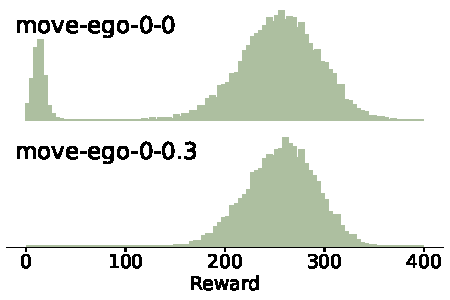
\includegraphics[width=.94\textwidth]{image/reward_hist_two_tasks_hist_simdr.pdf}
    %\end{figure}
\end{minipage}
\caption{\small Tracking, reward, and goal-reaching performance across models for different testing configurations (left), and example distributions of reward evaluation scores for \method{} in Isaac (DR) (right). Each metric is averaged over tasks. We consider the average return over episodes lasting 500 steps for reward, the average joint position error $E_{\mathrm{mpjpe}}$ averaged over the whole motion for tracking, and the error $E_{\mathrm{mpjpe}}$ averaged over the episode for goal-reaching.}
        \label{tab:sim.experiments}
\end{figure}


\subsection{Zero-shot Validation in Simulation}\label{ssec:sim.experiments}
\vspace{-3mm}
In this section, we quantitatively assess the performance and robustness of \method{} along different dimensions in simulation.

\textbf{Asymmetric learning and domain randomization.} We consider a \emph{privileged} version of \method{} where all components of the algorithm receive privileged information. We train this model in a simulated environment with nominal dynamical parameters (\emph{No DR}), and we test it in the very same configuration. This serves as an idealized configuration similar to the problems where unsupervised RL was previously shown to work~\citep{TirinzoniTFGKXL25zeroshot}, although it leads to a model that is \emph{not deployable} on the real robot. We then compare to \method{} trained and tested on a domain randomized version of the environment (\emph{Sim DR}), which corresponds to the model actually deployed on the real robot. Overall, \method{} is $2.47\%$, $25.86\%$, $10.65\%$ worse than \method{}-priv across tracking, reward, and pose reaching tasks. This shows that despite the algorithmic changes made in \method{} compared to FB-CPR, the learning dynamics is still correct and the model retains a satisfactory performance compared to its idealized version. Interestingly, reward tasks suffer from a larger drop in performance. This is in part due to the sparse nature of the reward functions we consider, which makes them less forgiving to suboptimal behaviors and amplify any model error. We also conjecture that this may be related to the reward inference process with domain randomized data. In Fig.~\ref{tab:sim.experiments} we also show the distribution of the performance of \method{} for two representative reward functions across repetitions of the inference process\footnote{In the reward inference, we use a dataset of states randomly subsampled from the training dataset. As a result, multiple repetitions of the process may return different policies.} and episodes. While for \texttt{move-ego-0.3} the performance is fairly consistent, for \texttt{move-ego-0.0}, we notice that a few instances obtained very poor performance. We conjecture that this is related to the increased randomness of the data observed during training due to domain randomization, which makes inference with a small subsampled dataset more brittle and prone to failure.


\textbf{Sim-to-sim performance.} We evaluate the robustness of \method{} to the dynamics of the humanoid by testing it in Mujoco. We notice that performance difference is limited (i.e., all variations are less than $7\%$), showing that the domain randomization at training and the history components in the actor and critics contribute to a good level of robustness and adaptivity.

\textbf{Out-of-distribution tasks.} Finally, we evaluate \method{} on a different set of tracking and pose reaching tasks obtained from the AMASS dataset~\citep{Mahmood2019AMASS}. We consider $175$ out-of-distribution motions from the CMU subset of the AMASS and $10$ manually-selected poses from the motions in the entire AMASS dataset. We run tests in Mujoco to combine different dynamics and out-of-distribution tasks. While a direct comparison of performance between LAFAN1 and AMASS tasks may be misleading due to the specific nature of the motions and poses used in the evaluation, we notice that overall \method{} is able to successfully generalize and complete tracking and pose reaching even when exposed to tasks that are not represented in the training data.

% \textbf{Test 1: What is the performance gap due to asymmetric learning?} 
% We want to investigate the impact of asymmetric learning in our unsupervised RL training where the space of rewards implicitly learned through $B$ and the regularized policy learning now leverage different information. We train a full privileged information model (\textsc{FB-CPR-oracle}) and compare it with one where the policy uses a history $s^h_t$ (\textsc{FB-CPR}). We train and test both models on the same simulation configuration with no form of domain randomization. \ale{Conjectured result is that the gap is ``small'' across all metrics.} \yitang{maybe also training curves}
% While asymmetric learning is an established approach for standard reward-based RL in robotics and partially-observable environments in general, no prior investigation is available on its impact in unsupervised RL and in particular in a complex algorithm FB-CPR, where the space of rewards implicitly learned through $B$ and the regularized policy learning now leverage different information. In order to assess the impact of asymmetric learning on the overall performance, we train a full privileged information model (\textsc{FB-CPR-oracle}) and compare it with one where the policy uses a history $s^h_t$ (\textsc{FB-CPR}). We train and test both models on the same simulation configuration with no form of domain randomization. \ale{Conjectured result is that the gap is ``small'' across all metrics.}

% \textbf{Test 2: Is domain randomization needed?} A typical approach to mitigate the sim-to-real gap is to train policies under perturbations both in the observation and in the simulator's dynamics in order to produce more robust behaviors. We assess the level of robustness of the learned policies by training \textsc{FB-CPR} with or without domain randomization, while then testing on the same environment but with domain randomization. We further test the trained models in a sim-to-sim scenario, where the underlying testing simulator is different from the training one. \ale{Conjectured result is that training without DR would perform very poorly when tested on an environment with DR both in sim and sim2sim.}

% \textbf{Test 3: Are models trained with domain randomization sufficiently robust?} While the previous tests show that history-dependent policies have a small gap w.r.t.\ learning with privileged information and domain randomization leads to behaviors that are more robust, the overall model is not capable of adaptation to the actual dynamics of the testing environment. We then train \textsc{FB-CPR-hist}, where all architectures use a history $s^h_t$. This gives to the critics, which already have access to the privileged state, the capability of adapting to non-observable aspects of the environment dynamics. \ale{Conjectured result is that the hist model works better than standard one and it has smaller variance across DR as it can better adapt to the specific dynamics instance in each episode.} \yitang{I think we can just compare model-vanila v.s. model+history+dr (dont need to separate dr and hist)}



% We consider 6 training configurations: asymmetric training, policy using privileged information and fully unprivileged (all models use only proprioceptive information), with and without domain randomization. These variations are used in the ablation studies to assess the impact of each component on the final performance. The only model test on the real-robot is the one with asymmetric training and domain randomization. The model without domain randomization was not safe to deploy on the real robot.



% \subsection{Sim-to-sim Validation}
% In simulation we ablate the impact of domain randomization and of the asymmetric training, we do not ablate the auxiliary reward since this is specifically designed for sim-to-real. To access whether there is a drop in performance due to the asymmetric training, as mentioned above, we train an oracle model (non-deployable) where the actor also uses privileged information. To assess the performance of the trained domain randomization across various environments, we create validation environments with different levels of domain randomization. We report the different configurations of domain randomization in Table~\ref{tab:domain_rand}. Furthermore, we evaluate the impact of domain randomization by testing the model in a sim-to-sim scenario where we evaluate the model on a simulated environment in DeepMind MuJoCo~\citep{TodorovET12}.

% \begin{table}[t]
%     \centering
%     \begin{tabular}{}
%     \end{tabular}
% \end{table}

% \textit{Downstream tasks and metrics.}
% The formal evaluation consists of three main categories:
% \begin{itemize}
% \item Reward Optimization: This category includes XXX reward functions designed to encourage a variety of behaviors. Performance is measured by the average return over episodes lasting 500 steps. 
% \item Goal Reaching: This category evaluates the model's ability to reach a specified goal starting from arbitrary initial conditions. We consider XXX manually selected ``stable'' poses. Two metrics are used: success rate, which measures whether the goal position is reached at any time, and proximity, which is the normalized average distance to the goal over time.
% \item Tracking: This category tests the model's ability to replicate a target motion beginning from its initial pose. A motion is deemed successfully tracked if the agent stays within a defined threshold of joint position and rotation distance from the target motion throughout its duration, as described in~\citep{LuoHYK21}. Additionally, the earth mover's distance~\citep[][EMD]{RubnerTG00} is used as a less-restrictive metric that does not require perfect time-alignment between the agent's trajectory and the target motion.
% \end{itemize}
% We furthermore present qualitative results showcasing the model's ability to perform motion in-betweeness, stitching and blending.

% We report the results of the ablation studies in Table~\ref{tab:sim2sim_results}. We summarize the main findings below.


% \paragraph{No performance loss due to asymmetric training.} {\color{red} Placeholder for results showing no significant drop in performance due to asymmetric training but loss if we use only proprioceptive information for training}

% \paragraph{No performance loss due to penalties.} {Penalties were a big thing we had to fight against. Should we demonstrate that we can recover the original performance with enough training?}

% \paragraph{Larger model performs better but requires more regularization.} {Larger models reached better metrics (and reached better results), but we had to penalize/dr them more. Maybe experiments to show this? E.g., non-penalized medium model > non-penalized residual model in sim2sim, but when penalized, the result is flipped?}

% \paragraph{Domain randomization improves robustness.} {\color{red} Placeholder for results showing that only the model trained with domain randomization perfoms well across all the DR configurations and simulators.}

% \paragraph{Sim-to-sim correlation with sim-to-real.} {Should we have a section on usefulness of sim2sim results for indicating what could work in sim2real? This is not actually helping our sim2real work at this point (too late), but as an insight this would be useful (e.g., how to setup the sim2sim in a way that reflects accurattely how the robot will work, and what things to track)}

% \paragraph{Qualitative evaluation.} {\color{red} Placeholder for qualitative results.}
% \vspace{-3pt}
\subsection{Zero-shot Validation on the Real Robot}

Finally, we deploy the \method{} model zero-shot on a real Unitree G1 robot. In real-world validation, we aim to \textbf{1)} qualitatively confirm the model's tracking, reward optimization, and goal reaching capabilities on a few selected tasks; \textbf{2)} assess its robustness to perturbations and failures (e.g., falling). \emph{All results in this section come from \textbf{one} model.}

% \ale{Explain more in detail the things we show in the videos}


%
\begin{figure}[t]
    \centering
    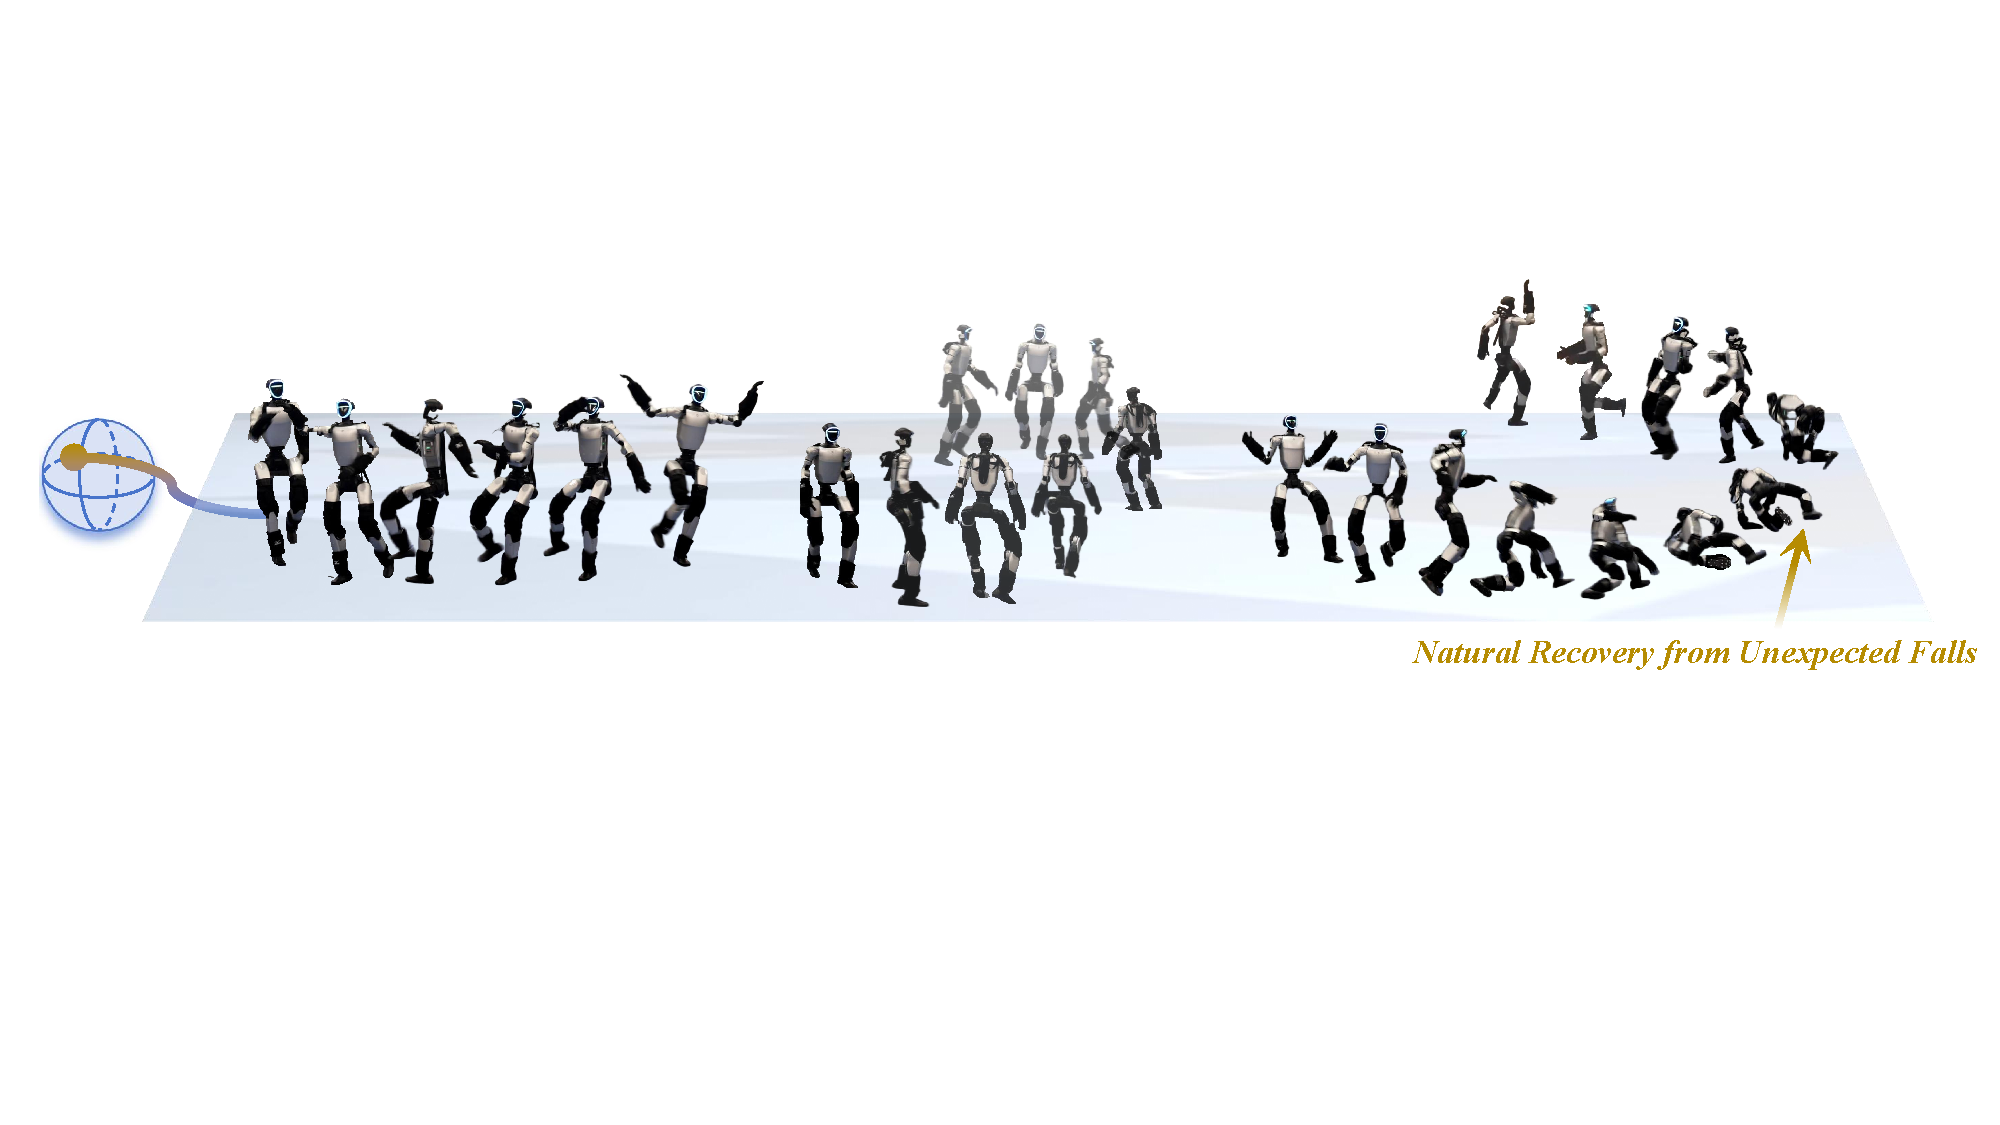
\includegraphics[width=\linewidth]{image/tracking_inference_1.pdf}
    \caption{Real-World Validation of \textbf{Tracking}. \emph{Left:} Highly dynamic dancing. \emph{Middle:} Frequently turning during walking. \emph{Right:} \textbf{Naturally} recover to continue track the motion.}
    \label{fig:tracking_inference}
\end{figure}
%
% it can track diverse motions, including xxxxx 
% it can track low quality ood motions in lalaland (even the motion is with some non continuous states)
% even not stable (falling down), it shows a very gental and natural behaviors during getting up, and keep tracking. not just robustness by trained with lots of disturbance, but truly have a human-like skill library by exposed to lots of motions that make it use some of the skills to continuously complete tracking 
% 
%
\textbf{Tracking.}
As shown in Fig.~\ref{figure_1_teaser} and Fig.~\ref{fig:tracking_inference}, \method{} enables the robot to track various motions, including styled walking motions, highly dynamic dances, fighting and sports. Even when becoming unstable or during a fall (\emph{Right}), it demonstrates remarkably gentle, natural, and safe behavior while recovering and continues tracking seamlessly. This capability stems not merely from robustness gained through disturbance training, but mostly from \emph{TD-based off-policy training} and the use of a GAN-based reward which explicitly encourages human-likeness and regularization terms that enable it to draw upon a rich skill library—much like a human—to adapt and complete tracking seamlessly. 
%
% the exposure to a wide range of human-like motions, enabling it to draw upon a rich skill library—much like a human—to adaptively complete the tracking task. 
%
% As shown in Figure~\ref{figure_1_teaser}, \ref{fig:tracking_inference}, \method{} enables robot to track diverse motions, including various walking styles, highly dynamic dances, fighting, and sports. Even when unstable or falling (\emph{Right}), it demonstrates remarkably gentle, natural, and safe behavior while recovering and continues tracking seamlessly. This capability stems not merely from robustness gained through extensive disturbance training, but from exposure to a wide range of human-like motions, enabling it to draw upon a rich skill library—much like a human—to adaptively complete the tracking task. 
%
Additionally, to evaluate the coverage and generalization capability, we used real videos and retargeted them to the G1.
%robot using~\citep{shen2024gvhmr,alhafez2023b}. 
Despite the suboptimal motion quality and discontinuities introduced by occlusions of monocular videos and artifacts in video estimation, the system is robust to lower quality data and can still successfully track these motions.

% As shown in Figure\ref{fig:tracking_inference}, our model can continuously track diverse motion within a single policy, including various walking styles, highly dynamic dances, fighting, and sports. 

% To test generalization, we evaluate out-of-distribution motions from AMASS and retargeted sequences from online sources. Even when mocap data is corrupted or low quality—producing fragmented trajectories—the model still tracks them effectively. In challenging motions where balance is lost, the robot can safely and naturally get up and resume tracking. This shows that our policy, with tracking-inference z, effectively handles out-of-tracking-state observations and produces natural recovery skills.

\textbf{Goal Reaching.}
%
\begin{figure}[t]
    \centering
    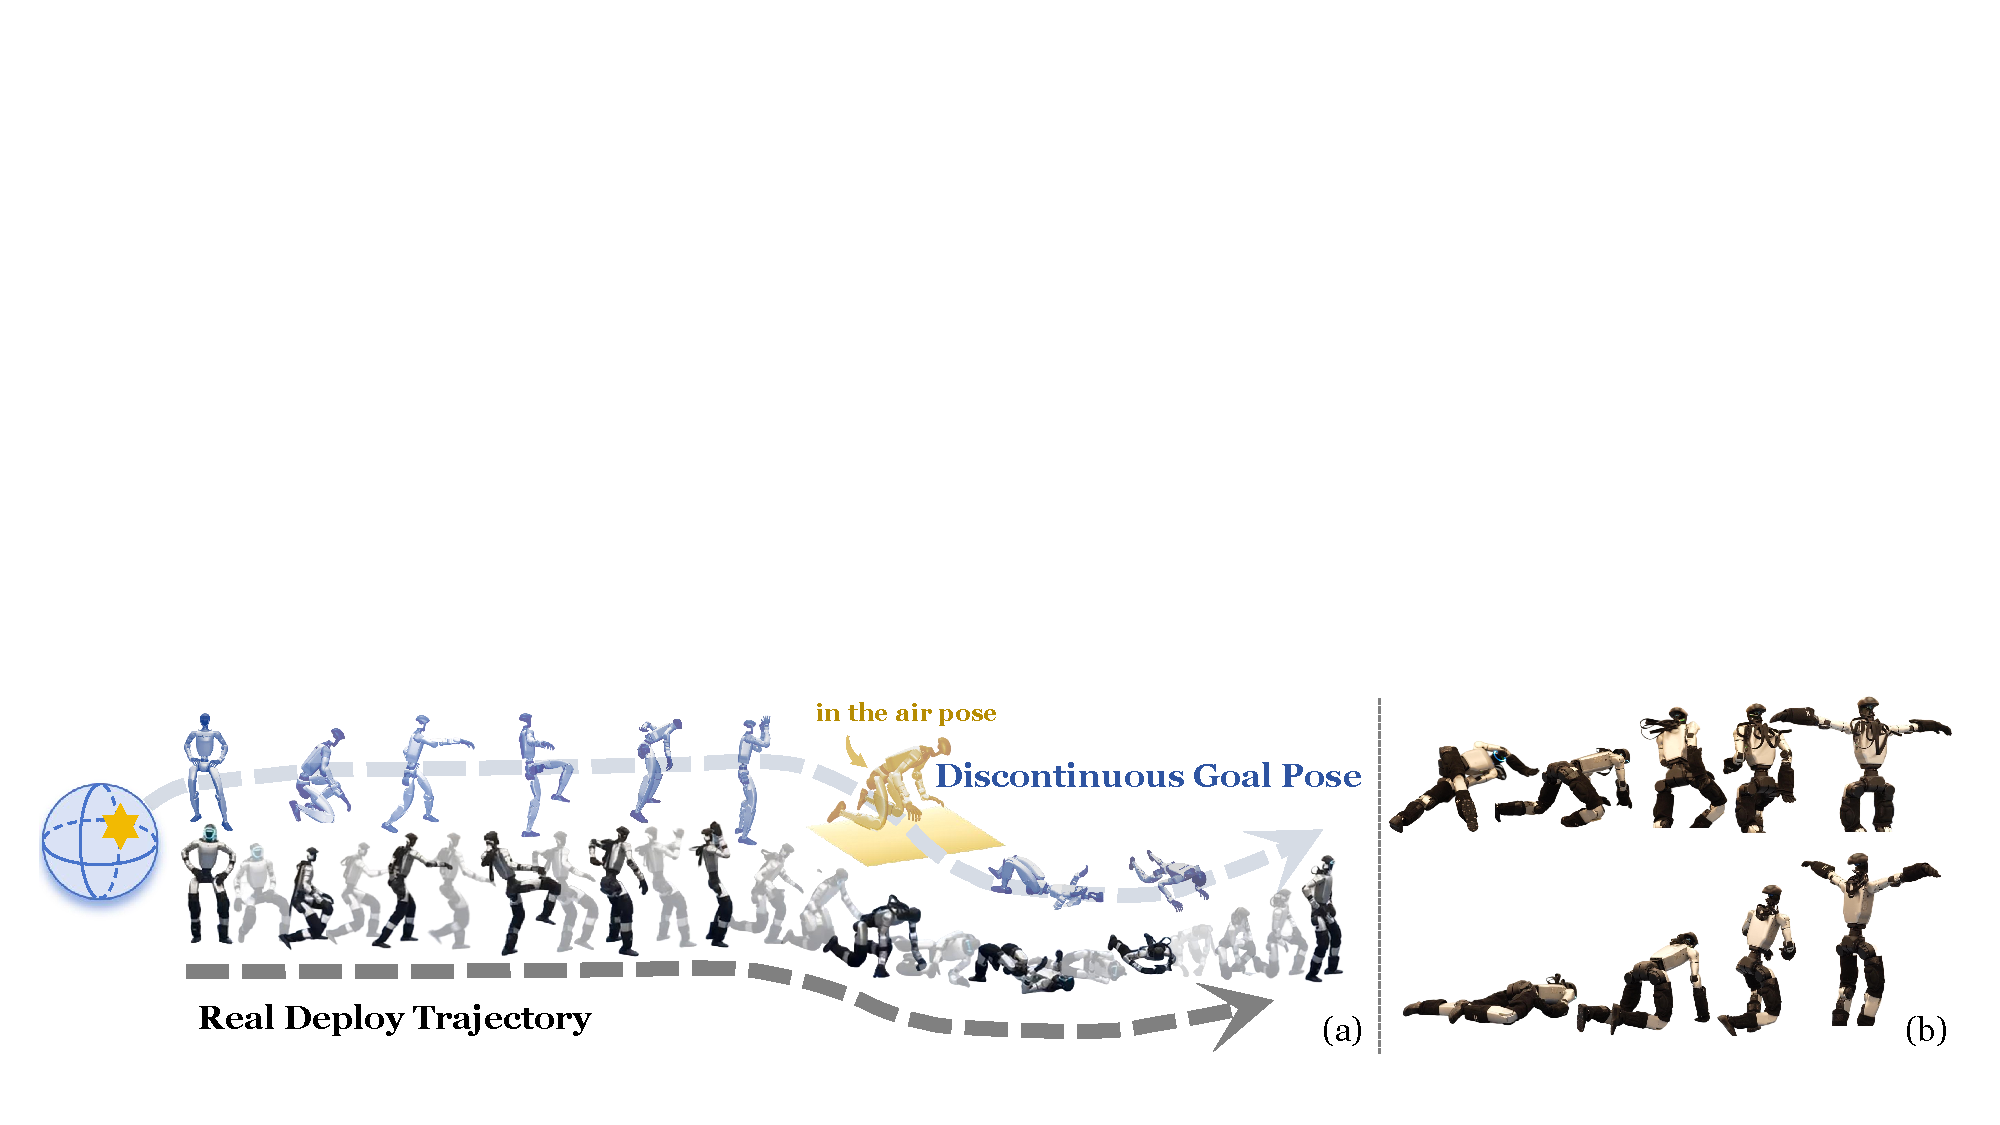
\includegraphics[width=\linewidth]{image/goal_reaching_final_1.pdf}
    \caption{\small Real-World Validation of \textbf{Goal Reaching}. (a) Continuously goal-reaching: the blue/yellow pose denotes the goal pose, while black marks the real robot pose, and gray visualizes the transition between each pose. (b) Transition from any pose to T-pose.}
    \label{fig:goal_inference}
\end{figure}
%
For the goal-reaching task, we extract a sequence of target poses by randomly sampling the goal states and discarding their velocity components. The zero-shot latent of these poses are then permuted and sequentially provided to the policy. As illustrated in Fig.~\ref{fig:goal_inference}, the robot consistently converges to a natural configuration that closely approximates the target pose, even when the target is infeasible (the Yellow one in Fig.~\ref{fig:goal_inference}). Moreover, the resulting trajectory exhibits smooth and natural transitions without the need for explicit interpolation, whether between successive and discontinuous targets(Fig.~\ref{fig:goal_inference}.a) or from an arbitrary pose to the T-pose(Fig.~\ref{fig:goal_inference}.b), demonstrating the smoothness of the learned skill space. 

% For the goal-inference task, we synthesize a sequence of target pose by randomly sampling goal states and discarding their velocity components. We can derive the latent for these quasi-static poses, permuted and presented to the policy in an arbitrary order. Figure~\ref{fig:goal_inference} demonstrates that the robot consistently converges to a natural configuration that approximates the—potentially infeasible—target. Furthermore, the trajectory exhibits smooth, natual between successive targets without requiring auxiliary interpolation schemes, thereby corroborating the implicit regularization conferred by the BFM latent manifold.

% For goal inference, we randomly generate some goal state with velocity values removed as target pose, and shuffle them in a sequence and sequentially reach them. As shown in Figure~\ref{fig:goal_inference}, the policy is able to reach a natural final pose close to the target, even when the target pose is not physically feasible. Moreover, without any explicit interpolation, it transitions smoothly from one pose to another, further highlighting the strong regularization properties of the BFM space.



\begin{figure}[t]
    \centering
    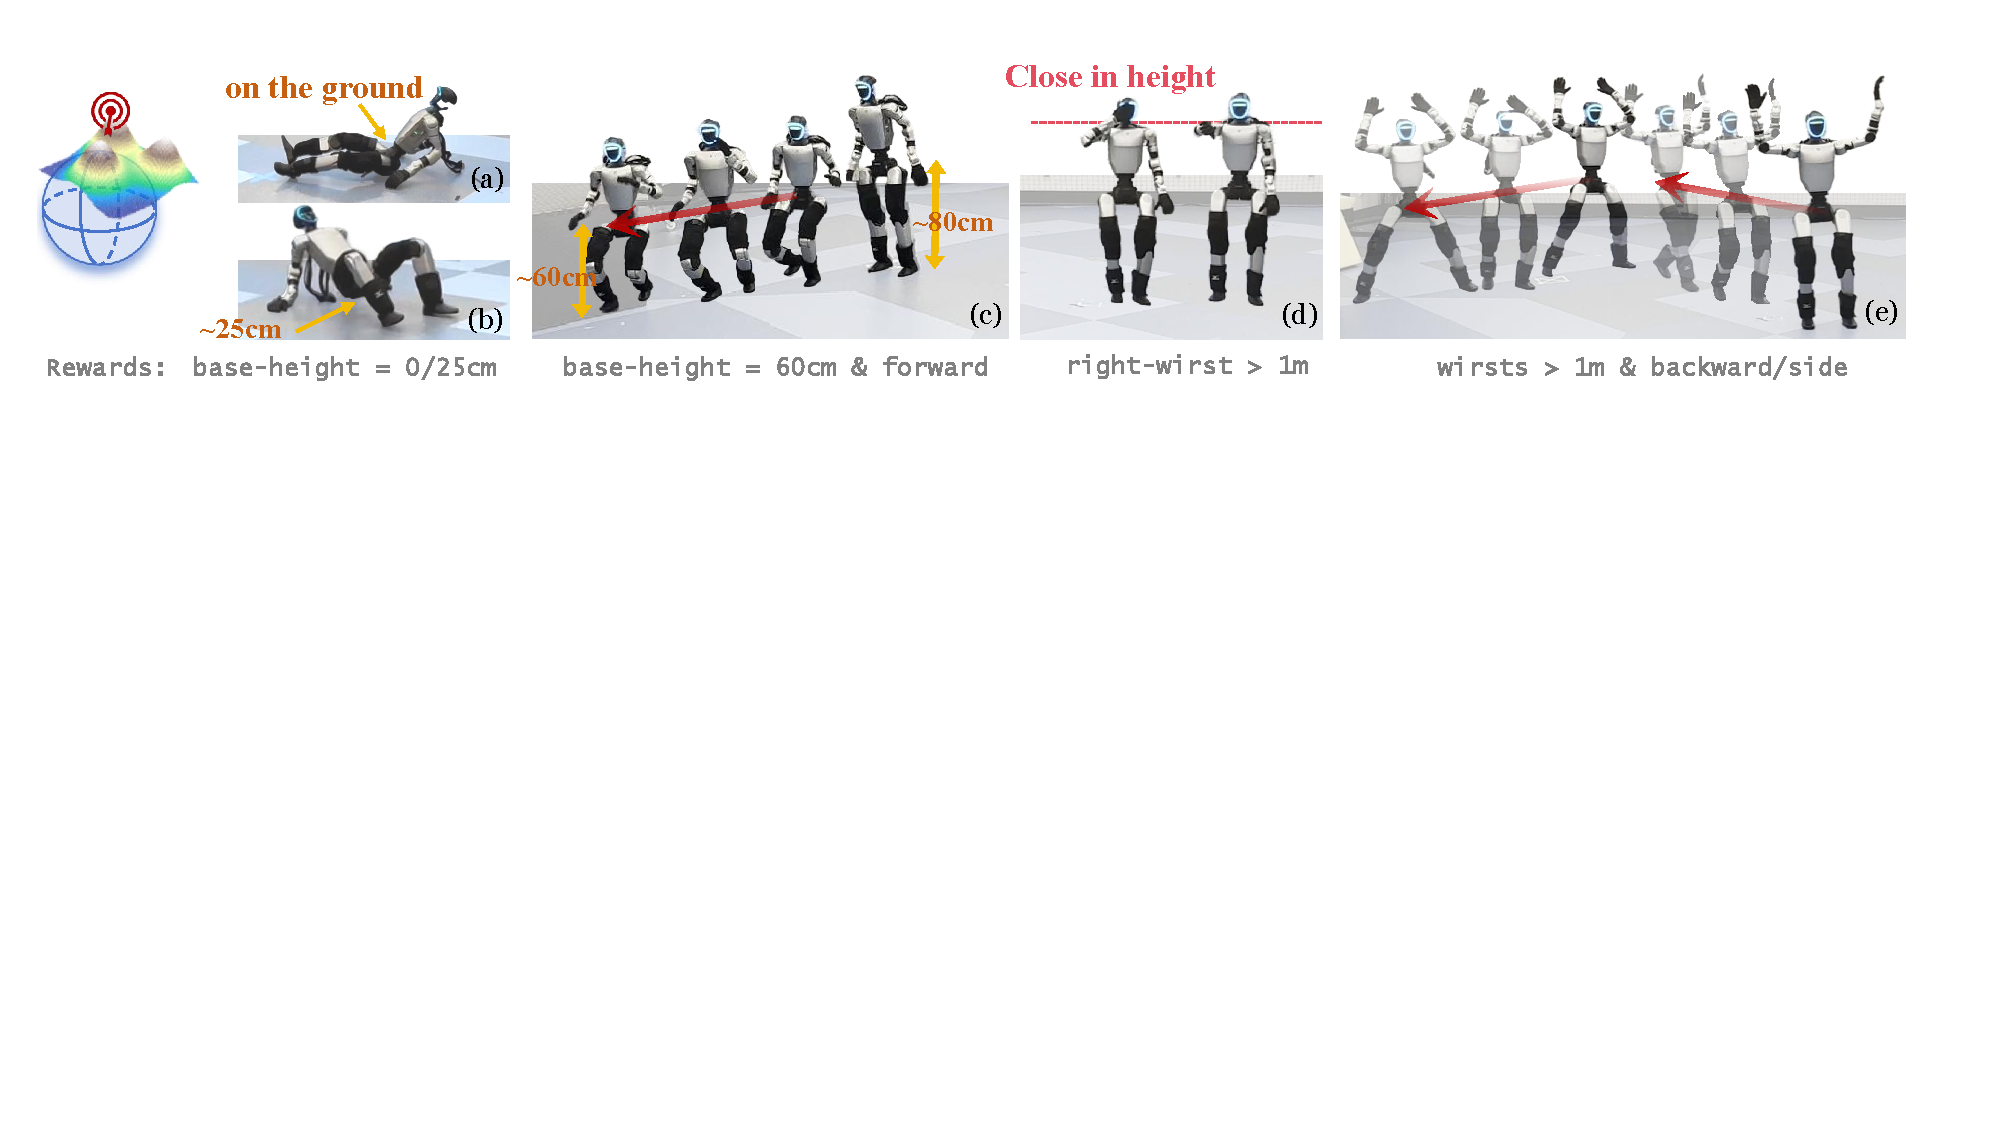
\includegraphics[width=\linewidth]{image/reward_optimization_final.pdf}
    \caption{\small Real-World \textbf{Reward Optimization}. The red arrow represents the base velocity tracking target. (a) \texttt{sitting}; (b) \texttt{crouch-0.25}; (c) \texttt{move-low0.6-ego-0-0.7}; (d) Diverse behaviors from \emph{one} reward \texttt{raisearm-m-l}; (e) combing \texttt{raisearm-m-l} with \texttt{move-ego-180-0.3} and \texttt{move-ego--90-0.7.}}
    \label{fig:reward_inference}
\end{figure}

% We evaluate reward inference in the real world with \emph{locomotion rewards} (moving and rotating, as shown in Figure~\ref{figure_1_teaser}), \emph{arm movement rewards}, and \emph{pelvis height control rewards} (sitting, crouching, or moving at low height, as shown in Figure~\ref{fig:reward_inference} (a,b,c)). All reward functions are defined in Appendix~\ref{app:rewards}. Even with simple reward definitions, the robot faithfully executes base-height, base-velocity, and arm-motion commands. Furthermore, we can get a combination of skills by simply combining rewards, enabling skill-level scaling and the emergence of novel behaviors.
% Also, testing the top-k latents instead of a weighted average reveals multiple behavior modes for loosely defined reward objectives(shown in Figure \ref{fig:reward_inference}(d)). With reward as objective formulation, our policy is friendly to language prompts and intuitive for human use.

% A single policy performs zero-shot inference across these diverse skills using reward-centric commands that are promptable and intuitive for human use. Testing the top-k latents instead of a weighted average reveals multiple behavior modes for loosely defined reward objectives. Moreover, by combining reward terms, the policy composes new skills on the fly, enabling skill-level scaling and the emergence of novel behaviors.
\textbf{Reward Optimization.}
We evaluate reward optimization in the real world with three task families: (i) locomotion rewards that specify base velocities and angular velocities, (ii) arm-movement rewards that command wrist height, and (iii) pelvis-height rewards that request sitting, crouching, or low-movement (Fig.~\ref{fig:reward_inference}(a–c)); reward definitions in Appendix~\ref{app:rewards}.
With simple reward definitions, the robot faithfully executes base-height, base-velocity, and arm-movement commands. Composite skills can be derived from simply linear combination of the rewards (e.g. going backward while raising arms), demonstrating controllable skill-level interpolability. Also, given a specific reward, averaging over different mini-batches from the replay buffer yields a set of latent variables that represents a diverse collection of potential optimal modes as shown in Fig.~\ref{fig:reward_inference}(d). Formulating objectives through reward functions makes our policy intuitive for human users and receptive to language prompts.


\begin{figure}[t]
    \centering
    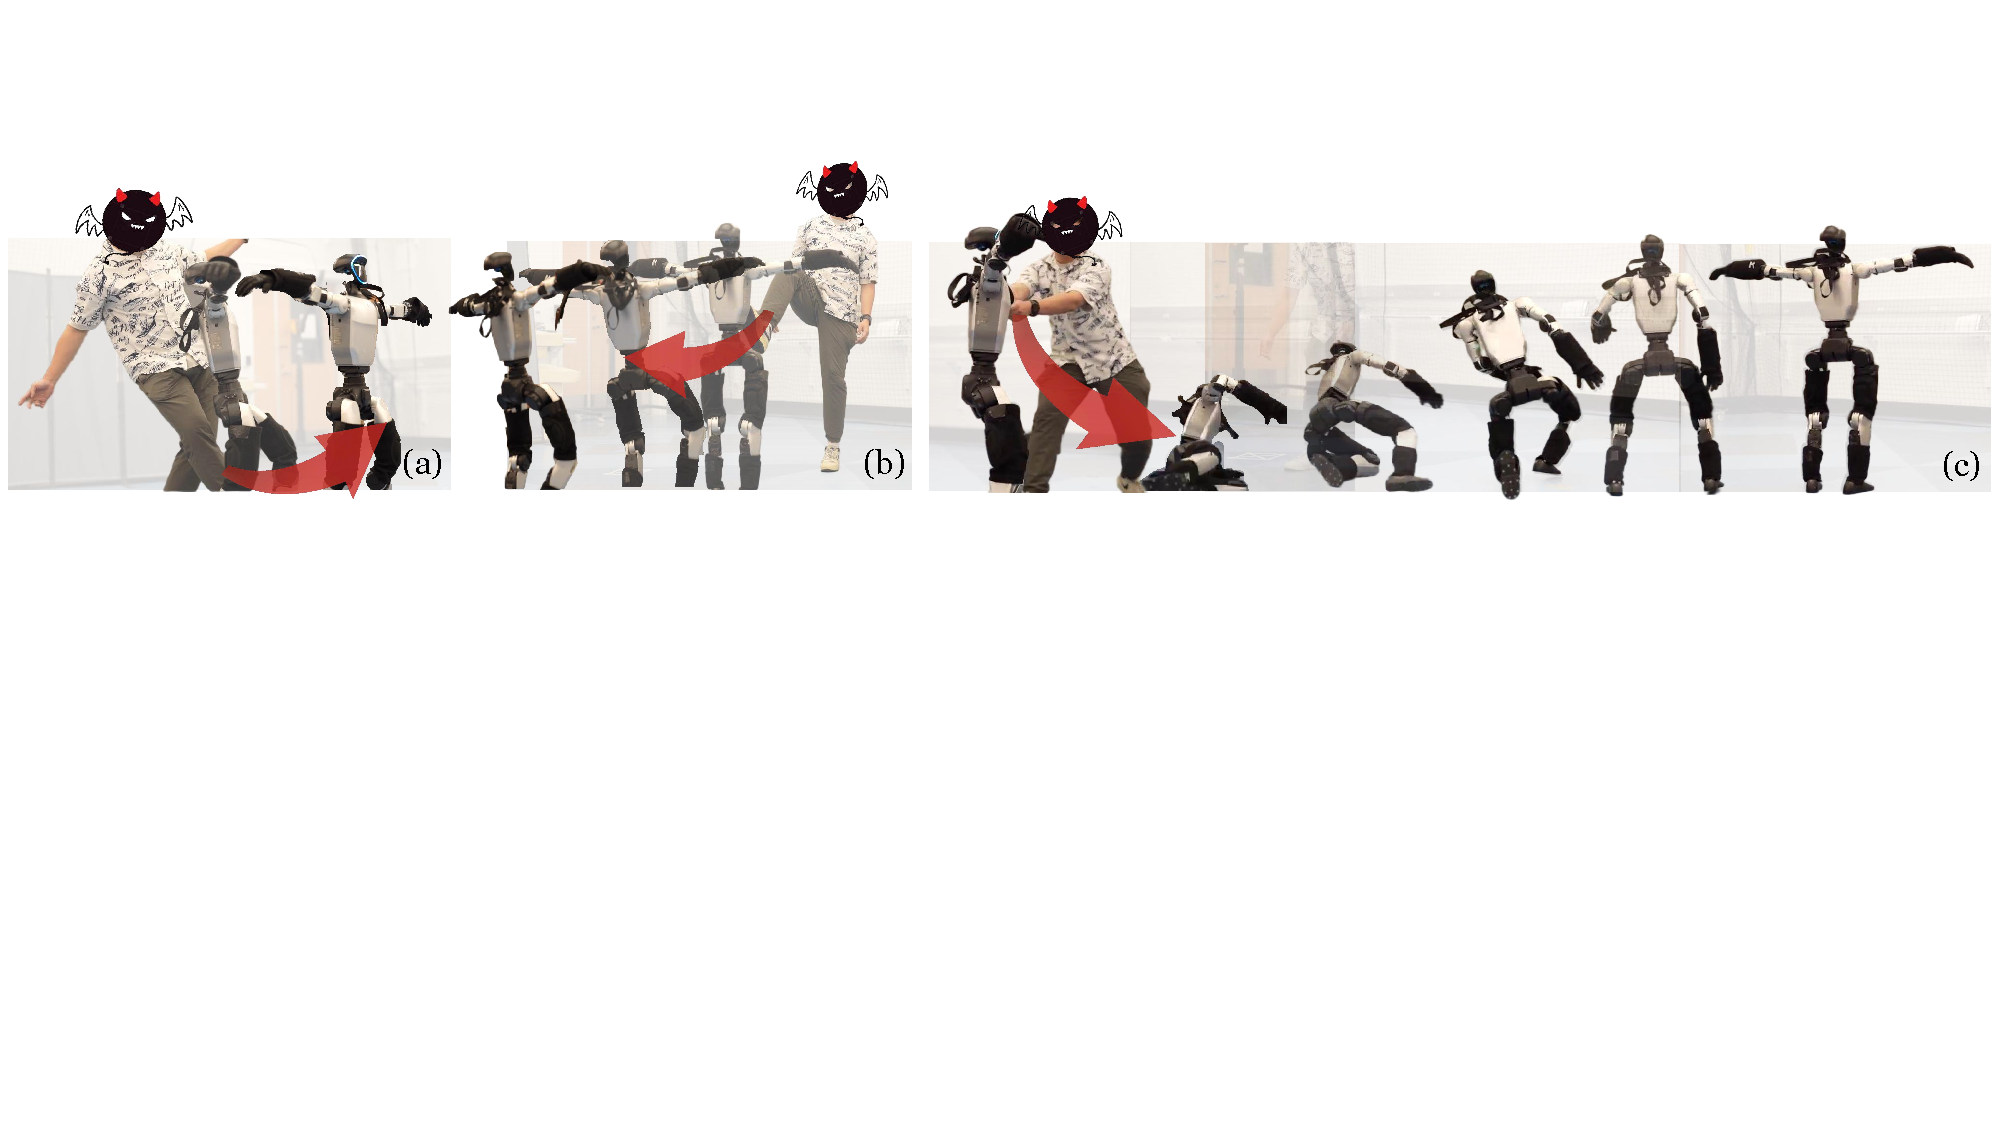
\includegraphics[width=\linewidth]{image/disturbance_rejection_1.pdf}
    \caption{\small Disturbance Rejection: (a) Keeps steady when kicked in the leg. (b) Absorbs a hard push with one smooth rear step. (c) \emph{Naturally} stands up and returns to T-pose after being yanked down.}
    \label{fig:disturbance}
\end{figure}
% One notable advantage of this policy is its compliance and robustness. As shown in Figure~\ref{fig:disturbance}, ~\ref{figure_2_teaser}, powered by our framework, the robot can react to strong disturbances such as fierce pushing, kicking, or being dragged to the ground in a human-like manner. After a strong forward push, it instinctively closes its arms, takes several quick steps in a running-like pose, then gradually slows down and reopens its arms (shown in Figure~\ref{figure_1_teaser}). \yitang{i want to stress this "robustness" and say better than unitree robustness testing demo} Although only a single latent vector from the static t-pose is always input to the policy, the policy will automatically and naturally deviate from the reference t-pose, takes a running-pose for recovery, before go back to track the t-pose, like a humand would do.
\textbf{Disturbance Rejection.}
One notable advantage of our policy is its strong compliance and robustness. As illustrated in Fig.~\ref{figure_1_teaser} and ~\ref{fig:disturbance}, our framework enables the robot to withstand severe disturbances—such as fierce pushes, kicks, or even being dragged to the ground, while recovering in a natural, human-like manner. For example, after a strong forward push, the robot instinctively closes its arms, takes several rapid steps in a running-like pose, and then slowly slows down before reopening its arms (Fig.~\ref{figure_1_teaser}). This level of robustness goes beyond the typical demonstrations seen in previous works: rather than fiercely reacting to the disturbances, our policy autonomously adapts. Although it receives only a single latent z from the static T-pose as input, it can automatically deviate from the reference posture, adopt a dynamic recovery pose, and eventually return to tracking the original T-pose just as a human would.

\begin{figure}[t]
    \centering
    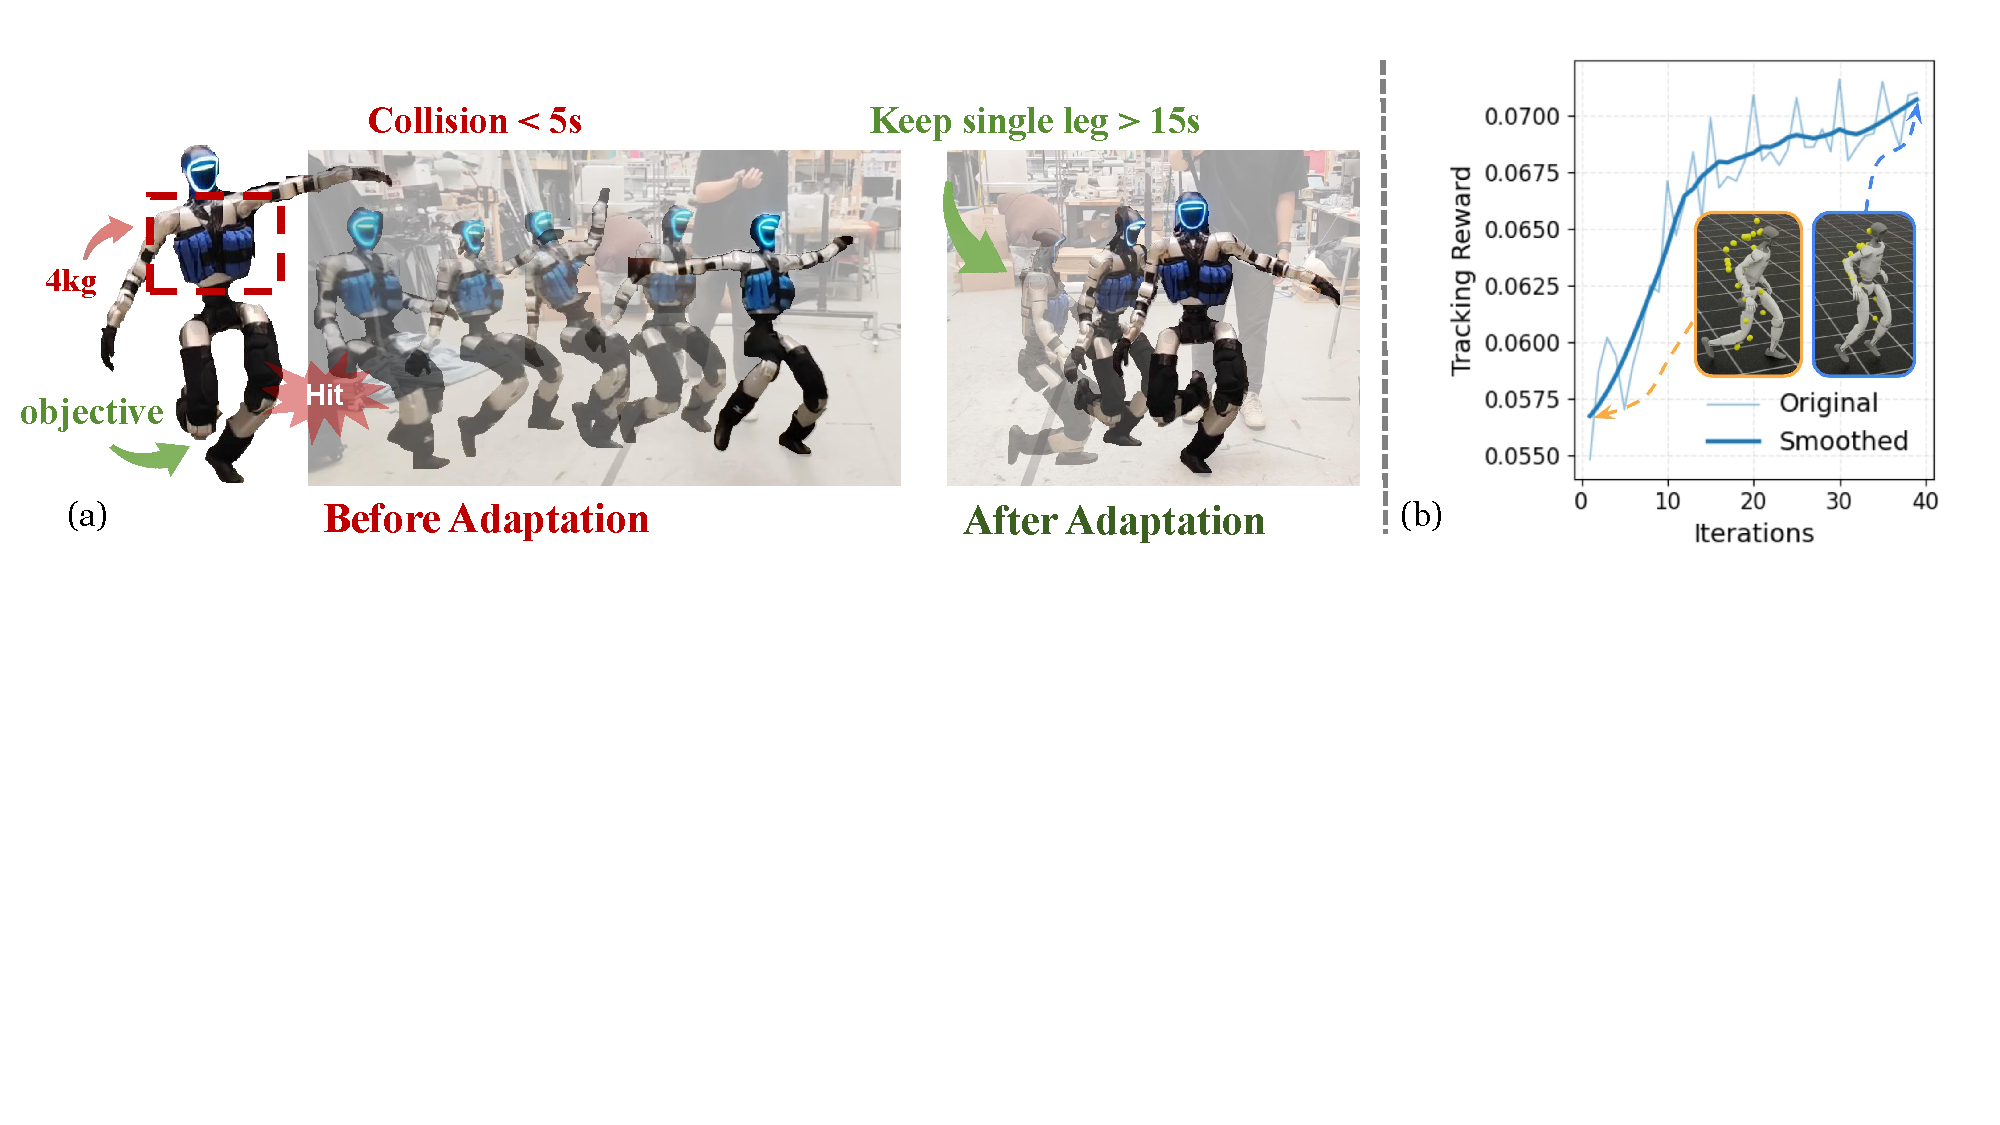
\includegraphics[width=.9\linewidth]{image/adaptation_final.pdf}
    \caption{Few-Shot Adaptation: (a) Single-pose adaptation improving single-leg standing under an additional payload. (b) Trajectory adaptation reduces tracking error.
}
    \label{fig:adaptation}
\end{figure}

\vspace{-0.3cm}

\subsection{Efficient Adaptation for \method{}}
\vspace{-2mm}
In this section we show how we leverage adaptation to improve the zero-shot inference performance under dynamics shift.
% \subsection{Visualizing the Latent Space of \method{}}

\textbf{Single Pose Adaptation.} We perform \emph{few-shot single-pose adaptation} in simulation to learn to stand on a single leg while carrying a payload. In simulation we increase the weight of the torso link by \textbf{4\,Kg}. Starting from the zero-shot latent $z^{\text{init}}$, we apply $20$ iterations of CEM to obtain $z^{\star}$, augmenting the rollout objective with a sparse task term $r\;=\;\mathbf{1}_{\{\,h_{\text{right foot}}>0.15~\mathrm{m}\ \wedge\ \text{no-contact}\,\}}$, 
which encourages right-foot clearance while avoiding unintended contacts. We deploy $z^\star$ on the real robot with a 4\,Kg mass rigidly attached to the torso.
As shown in~\Cref{fig:adaptation}\,(a), without adaptation, the motion driven by $z^{\text{init}}$ destabilizes and produces an environmental collision within $5\,\mathrm{s}$. In contrast, the optimized prompt $z^{\star}$ maintains single-leg balance for over $15\,\mathrm{s}$. These results indicate that prompt-level optimization alone can compensate for the payload-induced dynamics shift, without fine-tuning the model parameters.

\textbf{Trajectory Adaptation.}
For trajectory adaptation, we focus on optimizing a leaping motion under altered ground friction. We perform dual-annealing trajectory optimization \citep{xue2025full} in simulation using the explicit tracking reward defined in \citep{Luo2023phc}. We used sampling with particle count $N = 2048$, temperature schedules $\beta_{1} = 0.85$ and $\beta_{2} = 0.9$, and optimization iterations $M = 6$. The reward curve and before/after adaptation key-point tracking performance is shown in Fig.~\ref{fig:adaptation}(b), showing that our method significantly improves tracking accuracy, reducing error by $\sim$\emph{29.1}\%.

\subsection{The Latent Space Structure of \method{}}
\label{sec:latent}
\vspace{-2mm}
% \tonghe{This section may need another name? coz we also talk about interpolation.}\\
% \tonghe{
% Contact Tonghe for any questions in this part. 
% }\\
As mentioned in Sect.~\ref{sec:prelim}, \method{} provides an \textbf{interpretable} and \textbf{structured} representation of the behaviors of a humanoid robot. This representation not only facilitates understanding of the policy space but also enables instantaneous interpolation of existing skills without retraining. 

% \vspace{-2mm}
\textbf{Visualizing the Latent Space.}
 To examine the structure of the latent space, we sample latent vector trajectories and project them onto a two-dimensional plane (Fig.~\ref{fig:latent_z_map_2d}) to visualize the space, and also use a three-dimensional sphere to present representative latent generated for \emph{tracking, reward optimization and goal reaching}(Fig.~\ref{fig:latent_z_map_3d}) using t-SNE~\citep{tsne}. We can see the latent space is organized by motion style: semantically similar trajectories cluster, revealing a shared task centric structure.

% \begin{figure}[h]
%     \centering
%     \includegraphics[width=0.8\textwidth]{image/All-Tasks__tsne_3d_cropped.pdf}
%     \caption{t-SNE visualization of representative motions in 3D sphere.}
%     \label{fig:latent_z_map}
% \end{figure}
% \begin{figure}[h]
%     \centering
%     \includegraphics[width=0.8\textwidth]{image/All-Tasks_ts.pdf}
%     \caption{t-SNE visualization of representative motions in 2D plane.}
%     \label{fig:latent_z_map}
% \end{figure}

\begin{figure}[t]
    \centering
    \begin{subfigure}{0.3\textwidth}
        \centering
        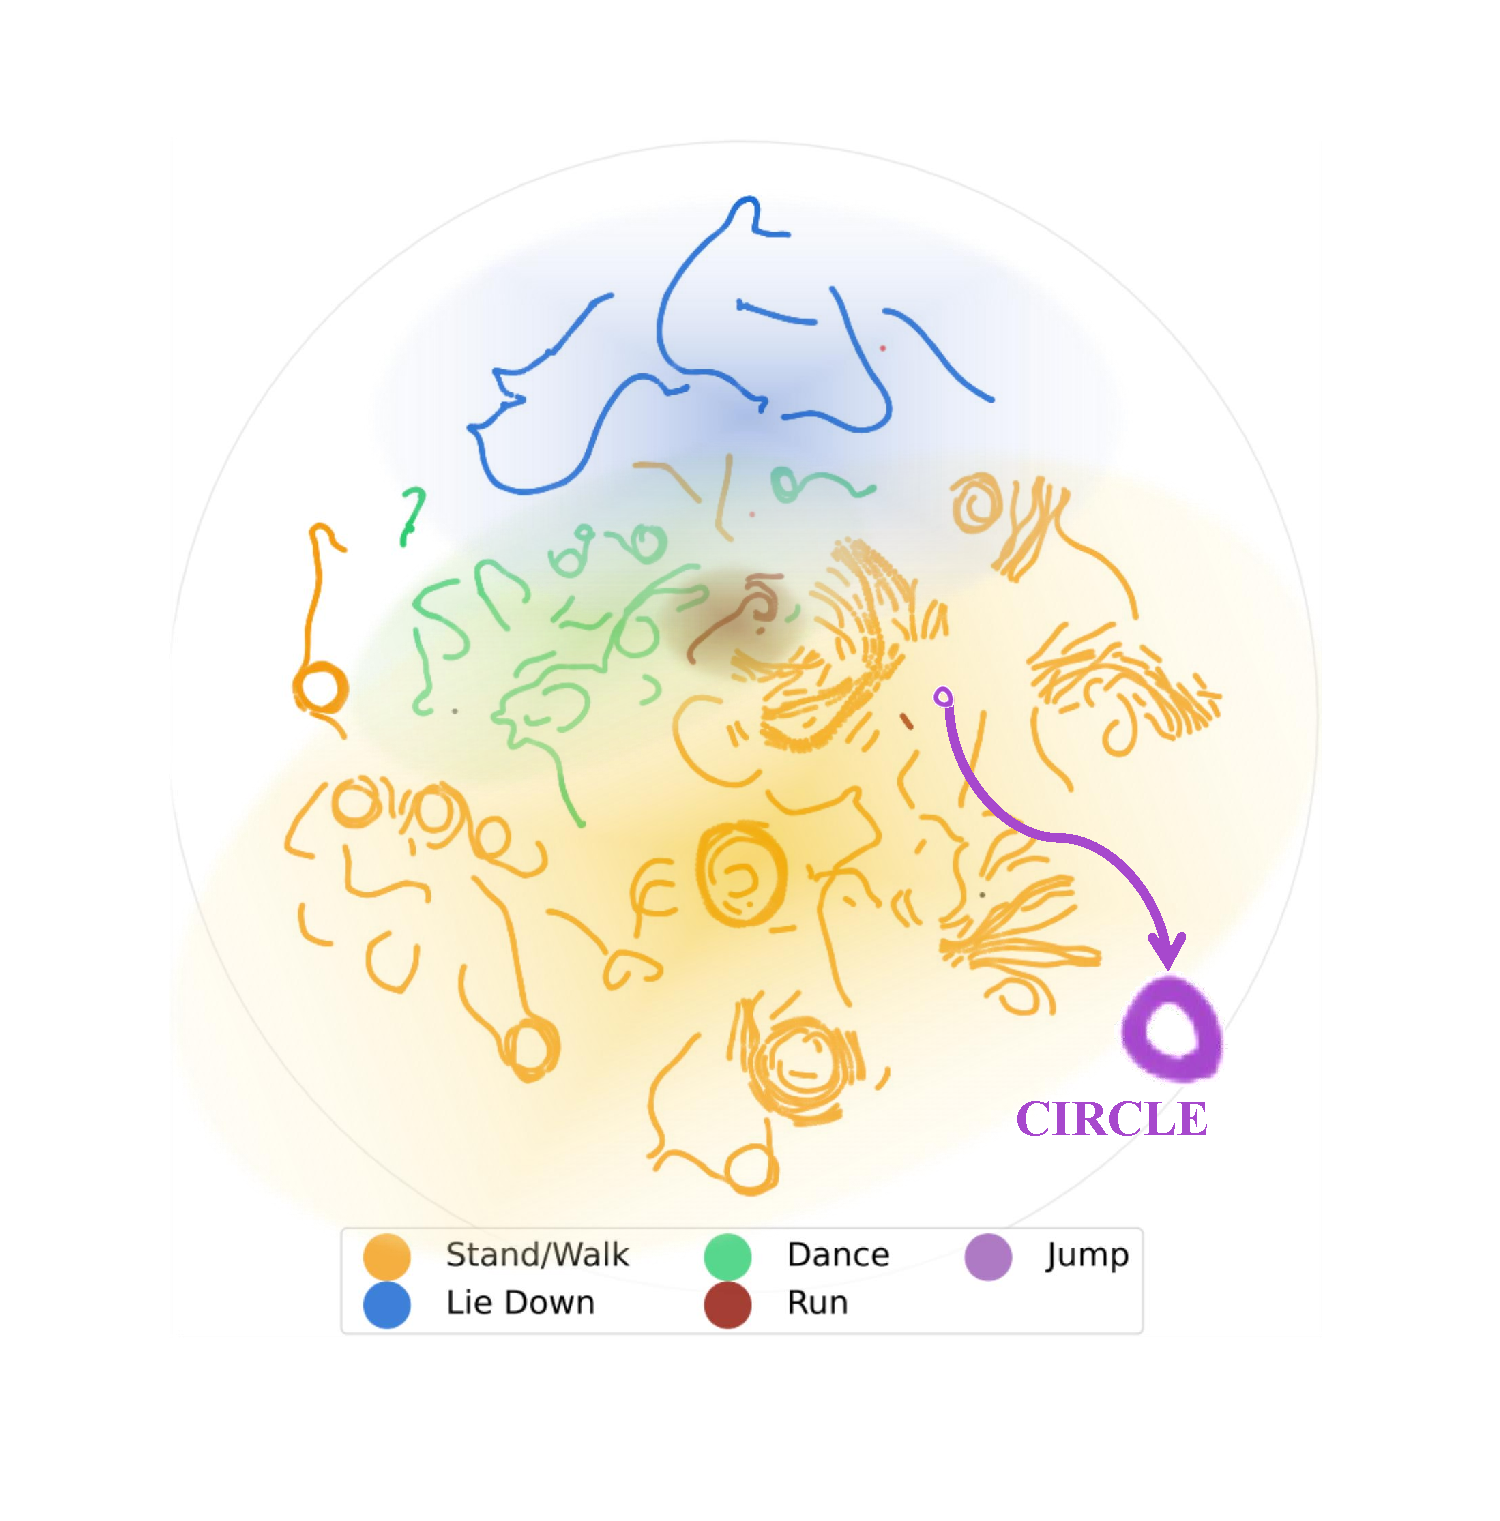
\includegraphics[width=.85\textwidth]{image/2d-tsne.pdf}
        \caption{Tracking trajectories segment the latent space (2D).}
        \label{fig:latent_z_map_2d}
    \end{subfigure}
      % \hfill
    \begin{subfigure}{0.32\textwidth}
        \centering
        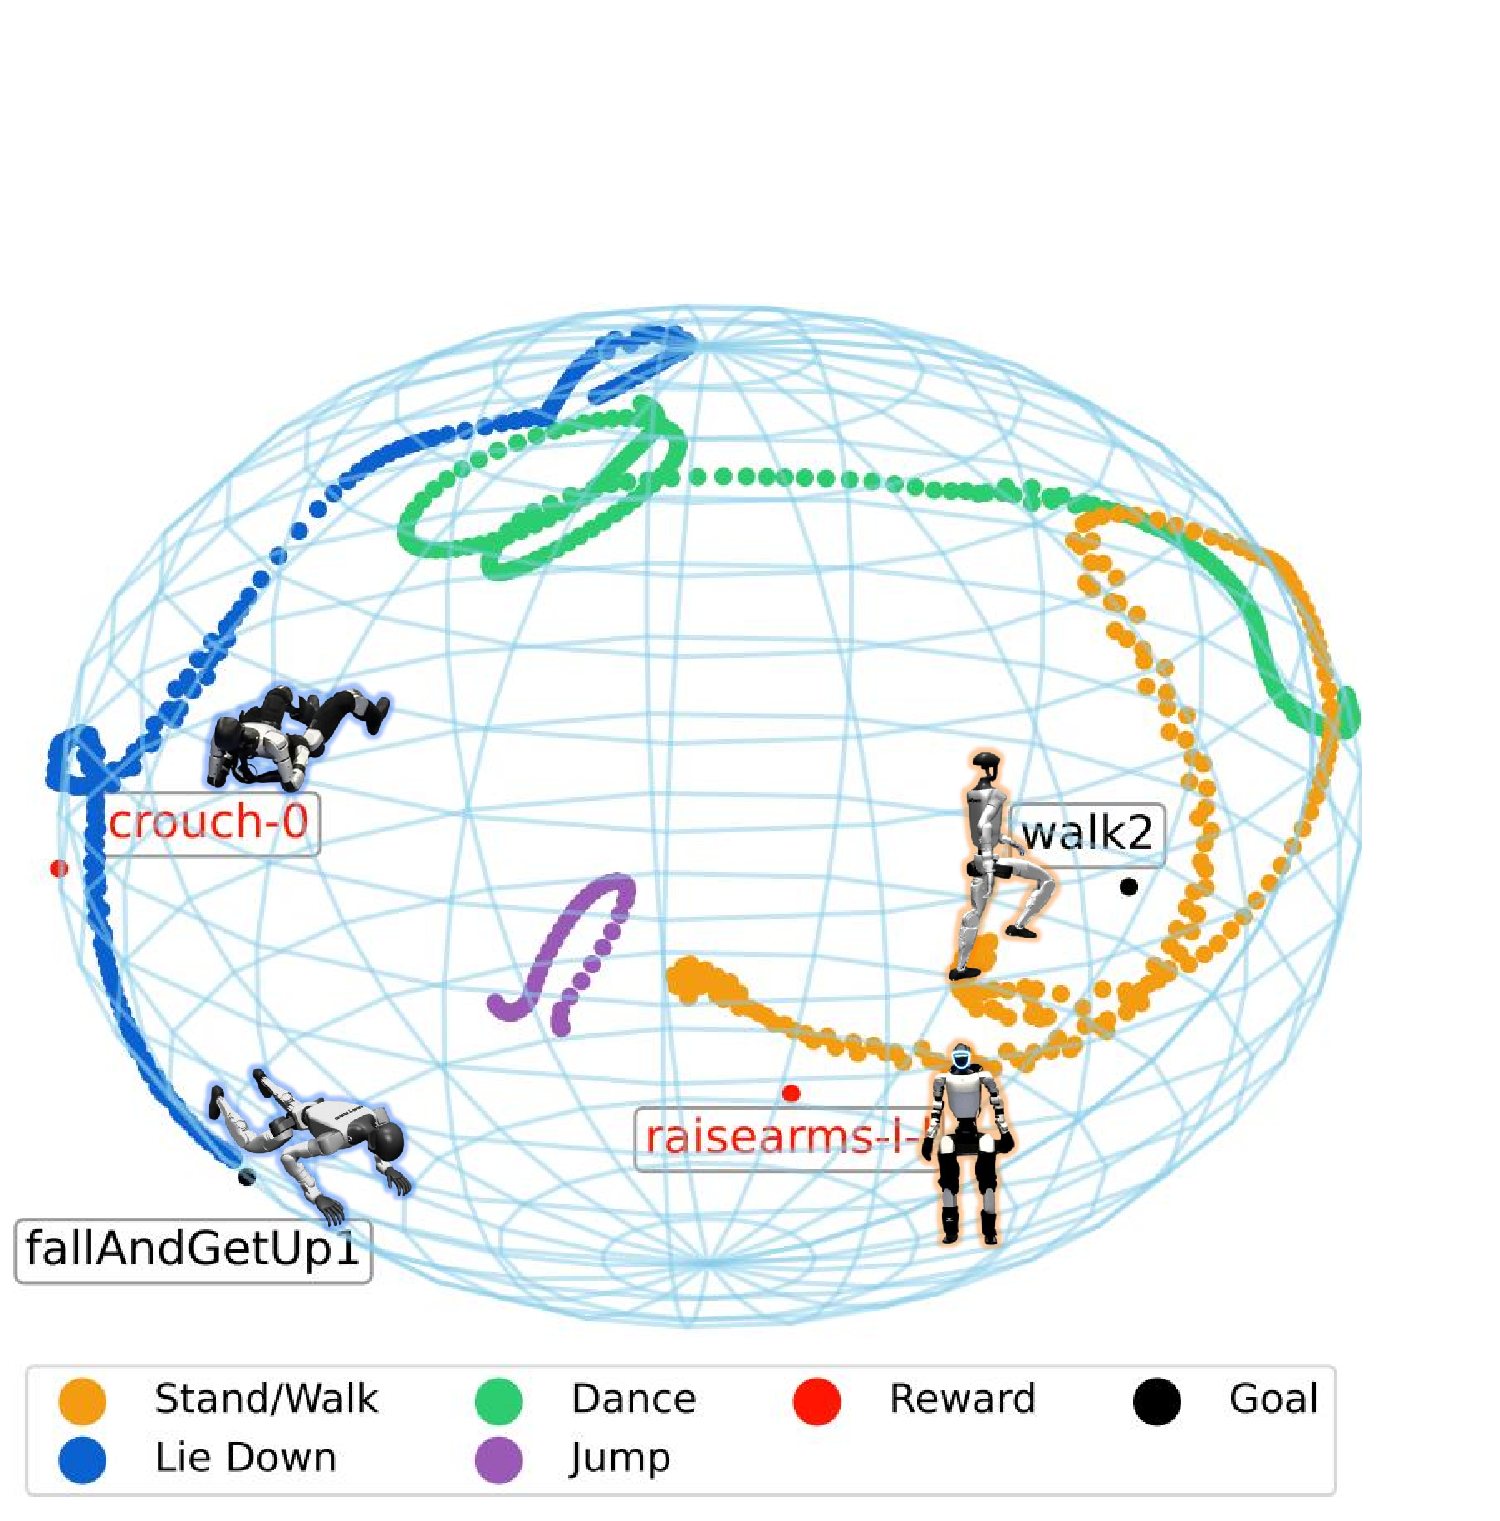
\includegraphics[width=.9\textwidth]{image/3d-tsne.pdf}
        \caption{Representative latents (3D).}
        \label{fig:latent_z_map_3d}
    \end{subfigure}
    \label{latent_z_map}
    \begin{subfigure}{0.28\textwidth}
        \centering
        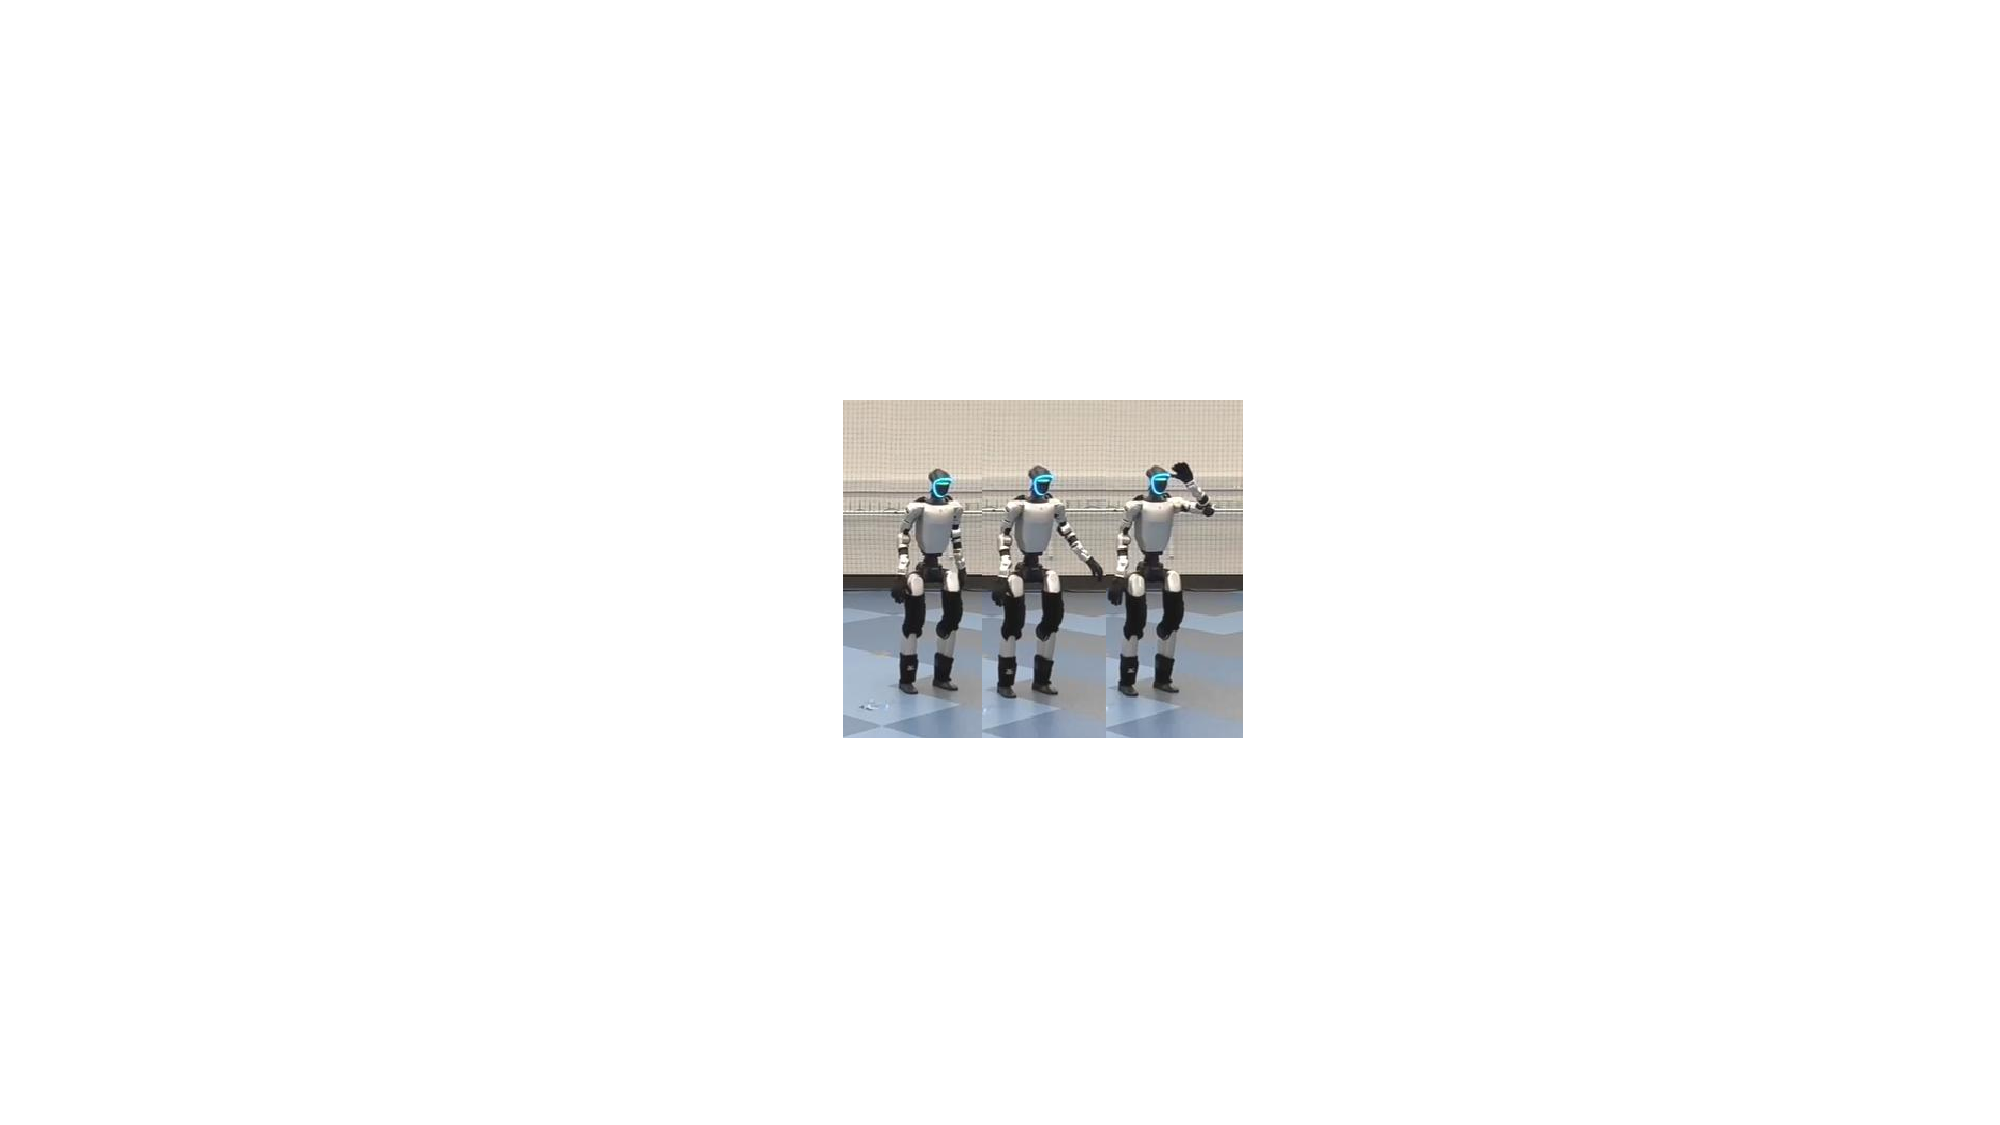
\includegraphics[width=\textwidth]{image/interpolation_final.pdf}
        \caption{Interpolation visualization}
        \label{fig:interpolation}
    \end{subfigure}
        \caption{Latent space visualization and analysis.}
\end{figure}
% \vspace{-2mm}
\textbf{Motion Interpolation on the Latent Space.}
The structured nature of $\mathcal{Z}$ enables smooth interpolation between latent representations. We can leverage Spherical Linear Interpolation~\citep{slerp} to generate intermediate latent vectors along the geodesic arc between the two end-points. To evaluate interpolated behaviors, we feed the resulting in-between $z_{t=0.5}$ into the \method{} policy, and deploy it on both simulated and real humanoid robots. As shown in Fig.~\ref{fig:interpolation}, the interpolated policy produces \emph{semantically meaningful} intermediate skills in a \emph{zero-shot} manner. These behaviors compose immediately—\emph{no additional training} required.

% The exact form of the interpolated points is specified by
% \begin{equation}
% \begin{aligned}
% z_{t} := \frac{\sin((1-t)\theta)}{\sin \theta}z_0 + \frac{\sin(t\theta)}{\sin \theta}z_1,
% \quad \theta := \arccos\left(\langle z_0, z_1 \rangle\right), \ z_0\ne z_1. 
% \end{aligned}
% \end{equation}
% for any interpolation parameter $t\in[0,1]$. 






\section{Discussion}\label{sec:discussion}
\vspace{-2mm}
In this paper we showed for the first time that off-policy unsupervised RL is a viable approach to train a behavioral foundation model for whole-body control of a real humanoid robot. While \method shows a remarkable level of generalization and robustness, it still suffers from several limitations: \textbf{1)} The scope and performance of the behaviors expressed by \method is connected to the motions used in training. Investigating the connection between the size of motion datasets, simulated datasets, architecture and model performance (e.g., quantity and quality of the learned behaviors) and consolidating it into scaling laws is important to guide future iterations of this approach. \textbf{2)} While history-based actor and critics and domain randomization reduced the sim-to-real gap, we believe algorithms with better online adaptation capabilities are needed to reliably express more complex movements. \textbf{3)} While we performed a preliminary investigation of test-time adaptation, a more thorough understanding of fast adaptation and fine-tuning of these models is needed to broaden their practical applicability.

\section{Acknowledgment}
\vspace{-2mm}
We would like to thank Tairan He and Haotian Lin for valuable discussions, and Chenyuan Hu for assistance with the experiments. Guanya Shi holds concurrent appointments as
an Assistant Professor at Carnegie Mellon University and as an Amazon Scholar. This paper describes work performed at Carnegie Mellon University and is not associated with Amazon.
%Another interesting venue is to enhance the algorithm with unsupervised exploration strategies to progressively expand its behaviors beyond the training motions. \textbf{2)} 
{
  % \bibliographystyle{iclr2026_conference}

\bibliography{iclr2026_conference}
\bibliographystyle{plainnat}
}
\newpage

\tableofcontents
\newpage
\appendix
\section{Related Work}
\label{sec:appendix-related-work}

In recent years, learning-based methods have made significant progress in whole-body control for humanoid robots. The largest body of work has focused on simulated humanoids. While these methods have demonstrated impressive capabilities in generating complex and dynamic behaviors using reinforcement learning~\citep{PengALP18deepmimic,Luo2023phc,Luo2024universal,TesslerGNCP24}, sim-to-real transfer remains a critical challenge in deploying learned policies on real-world humanoid robots. Various strategies have been proposed to bridge this gap, including domain randomization, system identification, asymmetric training, etc. However, the majority of these methods focus on single-task learning, where a policy is trained to perform a specific task, such as walking, running and get up~\citep{RadosavovicXZDMS24,Radosavovic2024nexttoken,Chen2024lipschitz,Seo2025fasttd3,Zakka2025mujocoplayground,he2025learninggettinguppoliciesrealworld}.

Recently, mostly 2025, there has been a surge of interest in developing multi-task and generalist humanoid control policies that can perform a wide range of tasks~\citep{He2024hover,he2025asap,Zhang2025humanoidreaching,zeng2025behaviorfoundationmodelhumanoid,Yin2025unitracker, Chen2025gmt}. The majority of these methods builds on top of approaches developed for simulated humanoids, and enhance them to be robust enough for sim-to-real transfer.
While ASAP~\citep{he2025asap} pre-train motion tracking policies in simulation and deploy them on the real robot to collect data to train a delta (residual) action model, the most common approach is to first train a motion tracking policy (or multiple policies) in simulation, and then distill it into a single multi-task policy that can perform all the skills in the motion dataset.
Common approaches for distillation include using a conditional variational autoencoder to learn a latent space of skills and doing online distillation~\citep{He2024hover,Yin2025unitracker,zeng2025behaviorfoundationmodelhumanoid,Chen2025gmt, Zhang2025humanoidreaching} or using diffusion models~\citep{liao2025beyondmimic}. However, all these methods require two stages of training to enable promptable policies, they are inherently limited by the quality of the motion since the base policies are trained to track the motion, and they relay on on-policy RL algorithms. Our method represents a significant departure from this paradigm by directly learning a promptable multi-task policy using an off-policy RL algorithm, which offer a much more reach and structured space of skills, and is not limited by the quality of the motion dataset.




% \section{Training Protocol}
% In this section we provide a description of the algorithm and training protocol.

\section{Training details}
\subsection{Training Hyperparameter Settings}
The agent interacts with the environment via episodes of fix length $T = 500$ steps. The algorithm has access to the dataset $\mathcal{M}$ containing observation-only motions. Similarly to~\citep{TirinzoniTFGKXL25zeroshot}, the initial state distribution of an episode is a mixture between randomly generated falling positions and states in $\mathcal{M}$ (motion initialization). We use prioritization to sample motions from $\mathcal{M}$ and, inside a motion, the state is uniformly sampled. We use an exponential prioritization scheme based on the agent's ability to track a motion. To have a more fine-grained prioritization, we split the $40$ LAFAN1~\citep{HarveyYNP20lafan1} motions into chunks of $10$ seconds. 
Every $N_{\mathrm{eval}}$ interaction steps, we evaluate all the motions and update the priorities base on the earth mover’s distance~\citep[EMD]{RubnerTG00}. For each motion $m \in \mathcal{M}$, the priority is given by
\[
p(m) \propto 2^{\max\Big\{0.5;\;\min\big\{\mathrm{EMD}(m), 2\big\}\Big\} \cdot 4}
\]

We take inspiration from the recipe in FastTD3~\citep{Seo2025fasttd3} to scale up unsupervised off-policy RL to using massively parallel environments. We use standard MLPs for all the components of the model, even for handling history. We simulate $N_{\mathrm{env}}$ parallel (and independent) environments at each step. We scale the buffer size accordingly to the number of environments, following the rule $N_{\mathrm{buffer}} \times N_{\mathrm{env}} \times T$. We use a batch size of $N_{\mathrm{batch}}$ and we use an update-to-data ratio of $N_{\mathrm{ups}}$ gradient steps per (parallel) environment step. We train the model for a total number of environment steps $N_{\mathrm{train}} = \frac{N_{\mathrm{grad}}N_{\mathrm{env}}}{N_{\mathrm{ups}}}$. We report the value of these parameters in Tab.~\ref{tab:params}, the missing parameters are as in~\citep{TirinzoniTFGKXL25zeroshot}.

% \begin{figure}[h]
% \begin{minipage}[t]{.48\textwidth}
\begin{table}[h]
    \centering
    \footnotesize % 缩小字体
    \begin{tabular}{lc}
    \toprule
    \textbf{Parameter} & \textbf{Value} \\
    \midrule
    \multicolumn{2}{l}{\textbf{Environment and Training Setup}} \\
    \midrule
    History Length $H$                  & 4 \\
    Episode Length $T$                  & 500 \\
    $N_{\mathrm{env}}$                  & 1024 \\
    $N_{\mathrm{batch}}$                & 1024 \\
    $N_{\mathrm{ups}}$                  & 16 \\
    $N_{\mathrm{grad}}$                 & 3M \\
    $N_{\mathrm{train}}$                & $\approx 192$M \\
    $N_{\mathrm{buffer}}$               & 10 \\
    $N_{\mathrm{eval}}$                 & $N_{\mathrm{train}}/20$ \\
    Buffer Size (transitions)           & $\approx 5$M \\
    Discount Factor                     & 0.98 \\
    Number of Seeding Steps             & $10 \cdot N_{\mathrm{env}}$ \\
    Fall Initialization Probability     & 0.3 \\
    \midrule
    \multicolumn{2}{l}{\textbf{Learning and Regularization}} \\
    \midrule
    Sequence Length (Trajectory Sampling) & 8 \\
    Latent Dimension $d$                 & 256 \\
    Discriminator Reg. Coef. $\alpha_D$  & 0.05 \\
    Reward Reg. Coef. $\alpha_R$         & 0.02 \\
    Gradient Penalty                     & 10 \\
    Learning Rate $F$                    & $3 \cdot 10^{-4}$ \\
    Learning Rate $B$                    & $10^{-5}$ \\
    Learning Rate $D$                    & $10^{-5}$ \\
    Learning Rate Actor $\pi$            & $3 \cdot 10^{-4}$ \\
    Learning Rate $Q_D$                  & $3 \cdot 10^{-4}$ \\
    Learning Rate $Q_R$                  & $3 \cdot 10^{-4}$ \\
    Orthonormality Loss Coefficient      & 100 \\
    \midrule
    \multicolumn{2}{l}{\textbf{Inference}} \\
    \midrule
    Number of samples for reward inference      & 400000 \\
    Tracking look ahead in sim & Seq. length\\
    Tracking look ahead in real& 3 (real)\\
    \bottomrule
    \end{tabular}
    \caption{Training settings.}
    \label{tab:params}
\end{table}
% \end{minipage}
% \end{figure}

% \end{wraptable}

\subsection{Network Architectures}
We use a residual architecture for the actor and the critics with blocks akin to those of transformer architectures~\citep{VaswaniSPUJGKP17}, involving residual connections, layer
normalization, and Mish activation functions~\citep{Misra20}. We use an ensemble composed of two networks for critics. For discriminator and backward map we use a standard MLP with ReLu activation (see Fig.~\ref{fig:architectures}). Refer to Tab.~\ref{tab:archi} for more details.

\begin{figure}[h]
    \begin{minipage}{\textwidth}
        \centering
        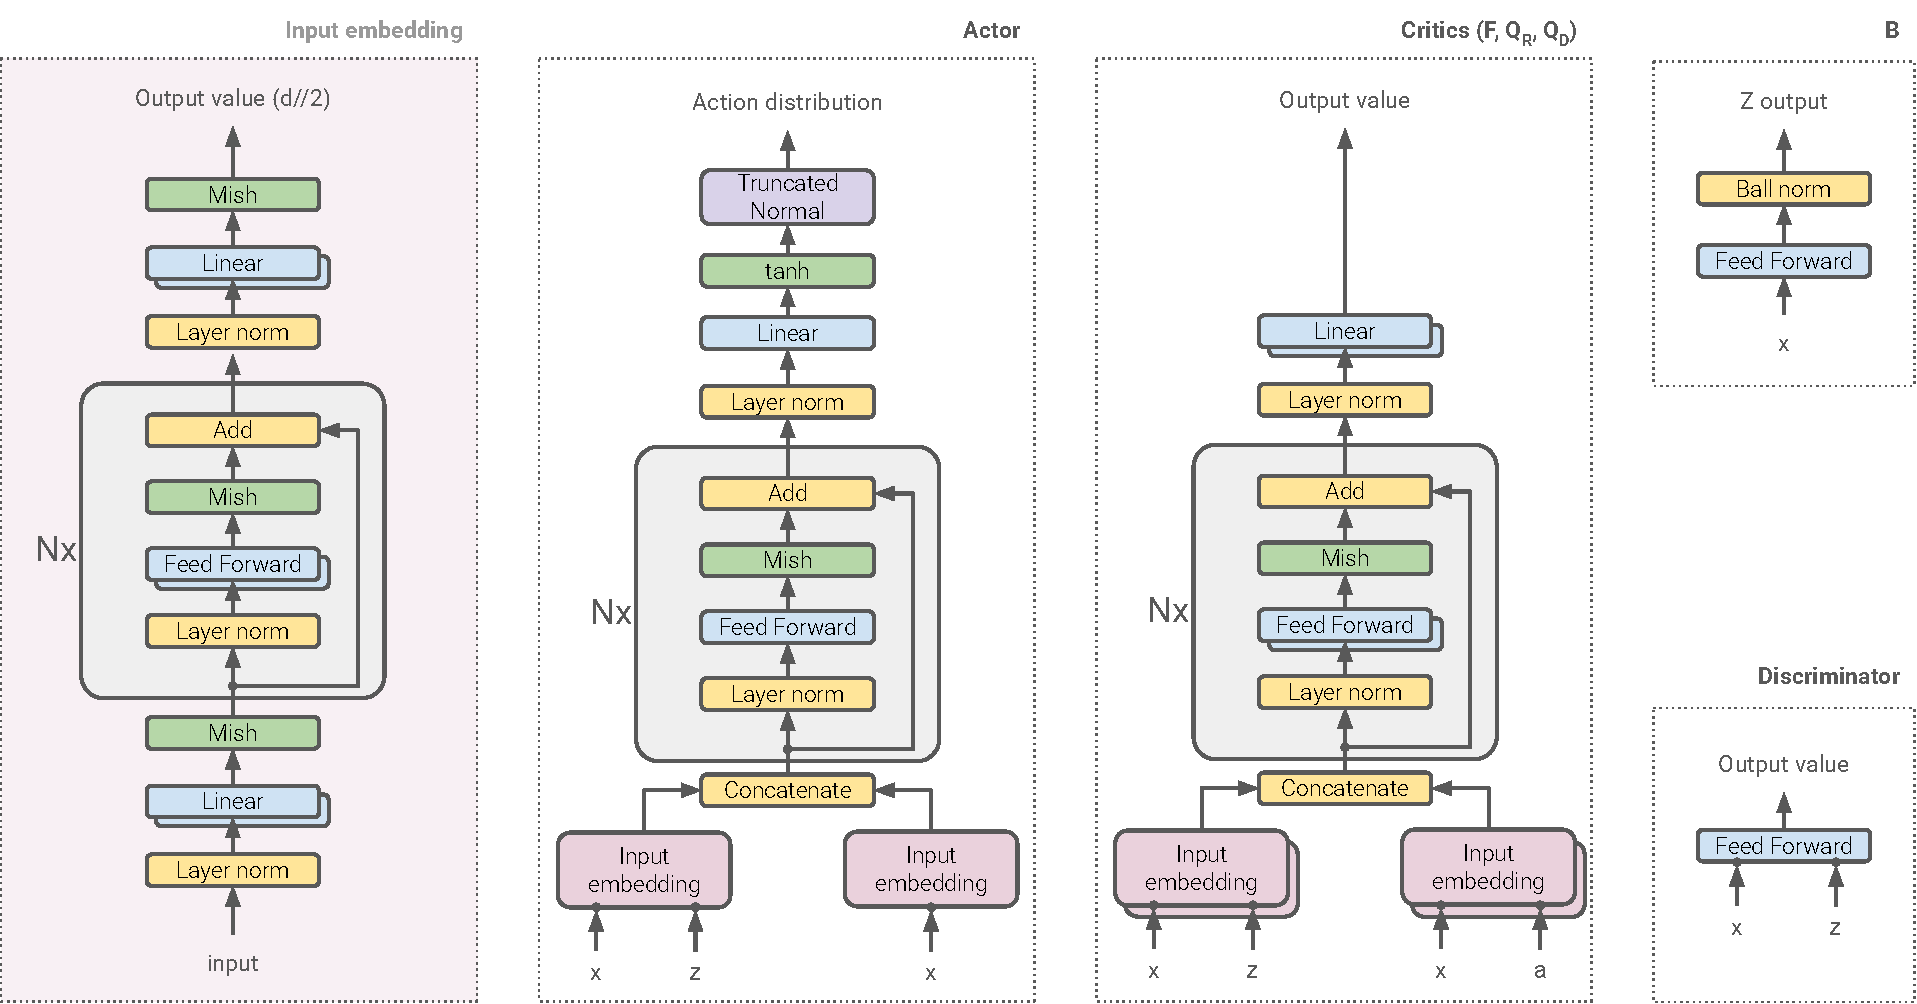
\includegraphics[width=0.9\linewidth]{image/architectures}
        \caption{Visual representation of the network architectures.}
        \label{fig:architectures}
    \end{minipage}
    % \\[.2in]
    % \begin{minipage}{\textwidth}
    %     \centering
    %     \footnotesize % 表格字体整体缩小
    %     \begin{tabular}{lcccc}
    %     \toprule
    %     \textbf{Hyperparameter} & \textbf{Critics (F, $Q_D$, $Q_R$)} & \textbf{Actor} & \textbf{Discriminator} & \textbf{B} \\
    %     \midrule
    %     Input Variables                & $(x, a, z)$ & $(x, z)$ & $(x, z)$ & $(x)$ \\
    %     Output Dim                     & F: $d$, $Q_D, Q_R$: 1 & 29 & 1 & $d$ \\
    %     Observation Variable $x$       & $(o_{t,H}, s_t)$ & $o_{t,H}$ & $(s_t, o_t)$ & $(s_t, o_t)$ \\
    %     Embedding Residual Blocks      & 4 & 4 & – & – \\
    %     Embedding Hidden Units         & 2048 & 2048 & – & – \\
    %     Residual Blocks                & 6 & 6 & – & – \\
    %     Feed Forward Hidden Layers     & 1 & 1 & 2 & 1 \\
    %     Feed Forward Hidden Units      & 2048 & 2048 & 1024 & 256 \\
    %     Activations                    & Mish & Mish & ReLU & ReLU \\
    %     Number of Parallel Networks    & 2 & 1 & 1 & 1 \\
    %     \midrule
    %     Num. Parameters (no target)    & F: 135.8M, $Q_D, Q_R$: 134.8M & 31.9M & 2.9M & 0.2M \\
    %     \midrule
    %     \textbf{Total Parameters}      & \multicolumn{4}{c}{\textbf{440.5M}} \\
    %     \bottomrule
    %     \end{tabular}
    %     \caption{Network architecture parameters used for real tests. $s_t$ is the privileged information and $o_t$ is the proprioceptive information. $o_{t,H} = \{o_{t-H}, a_{t-H}, \ldots, o_t\}$ denotes the history of proprioceptive states and actions. We exclude target networks when counting the number of parameters.}
    %     \label{tab:archi}
    % \end{minipage}
\end{figure}

\begin{table}[htbp]
    \centering
    \footnotesize
    \begin{tabular}{lcccc}
        \toprule
        \textbf{Hyperparameter} & \textbf{Critics (F, $Q_D$, $Q_R$)} & \textbf{Actor} & \textbf{Discriminator} & \textbf{B} \\
        \midrule
        Input Variables                & $(x, a, z)$ & $(x, z)$ & $(x, z)$ & $(x)$ \\
        Output Dim                     & F: $d$, $Q_D, Q_R$: 1 & 29 & 1 & $d$ \\
        Observation Variable $x$       & $(o_{t,H}, s_t)$ & $o_{t,H}$ & $(s_t, o_t)$ & $(s_t, o_t)$ \\
        Embedding Residual Blocks      & 4 & 4 & – & – \\
        Embedding Hidden Units         & 2048 & 2048 & – & – \\
        Residual Blocks                & 6 & 6 & – & – \\
        Feed Forward Hidden Layers     & 1 & 1 & 2 & 1 \\
        Feed Forward Hidden Units      & 2048 & 2048 & 1024 & 256 \\
        Activations                    & Mish & Mish & ReLU & ReLU \\
        Number of Parallel Networks    & 2 & 1 & 1 & 1 \\
        \midrule
        Num. Parameters (no target)    & F: 135.8M, $Q_D, Q_R$: 134.8M & 31.9M & 2.9M & 0.2M \\
        \midrule
        \textbf{Total Parameters}      & \multicolumn{4}{c}{\textbf{440.5M}} \\
        \bottomrule
    \end{tabular}
    \caption{Network architecture parameters used for real tests. $s_t$ is the privileged information and $o_t$ is the proprioceptive information. $o_{t,H} = \{o_{t-H}, a_{t-H}, \ldots, o_t\}$ denotes the history of proprioceptive states and actions. We exclude target networks when counting the number of parameters.}
    \label{tab:archi}
\end{table}

% \begin{figure}[t]
%     \begin{minipage}{\textwidth}
%     \centering
%     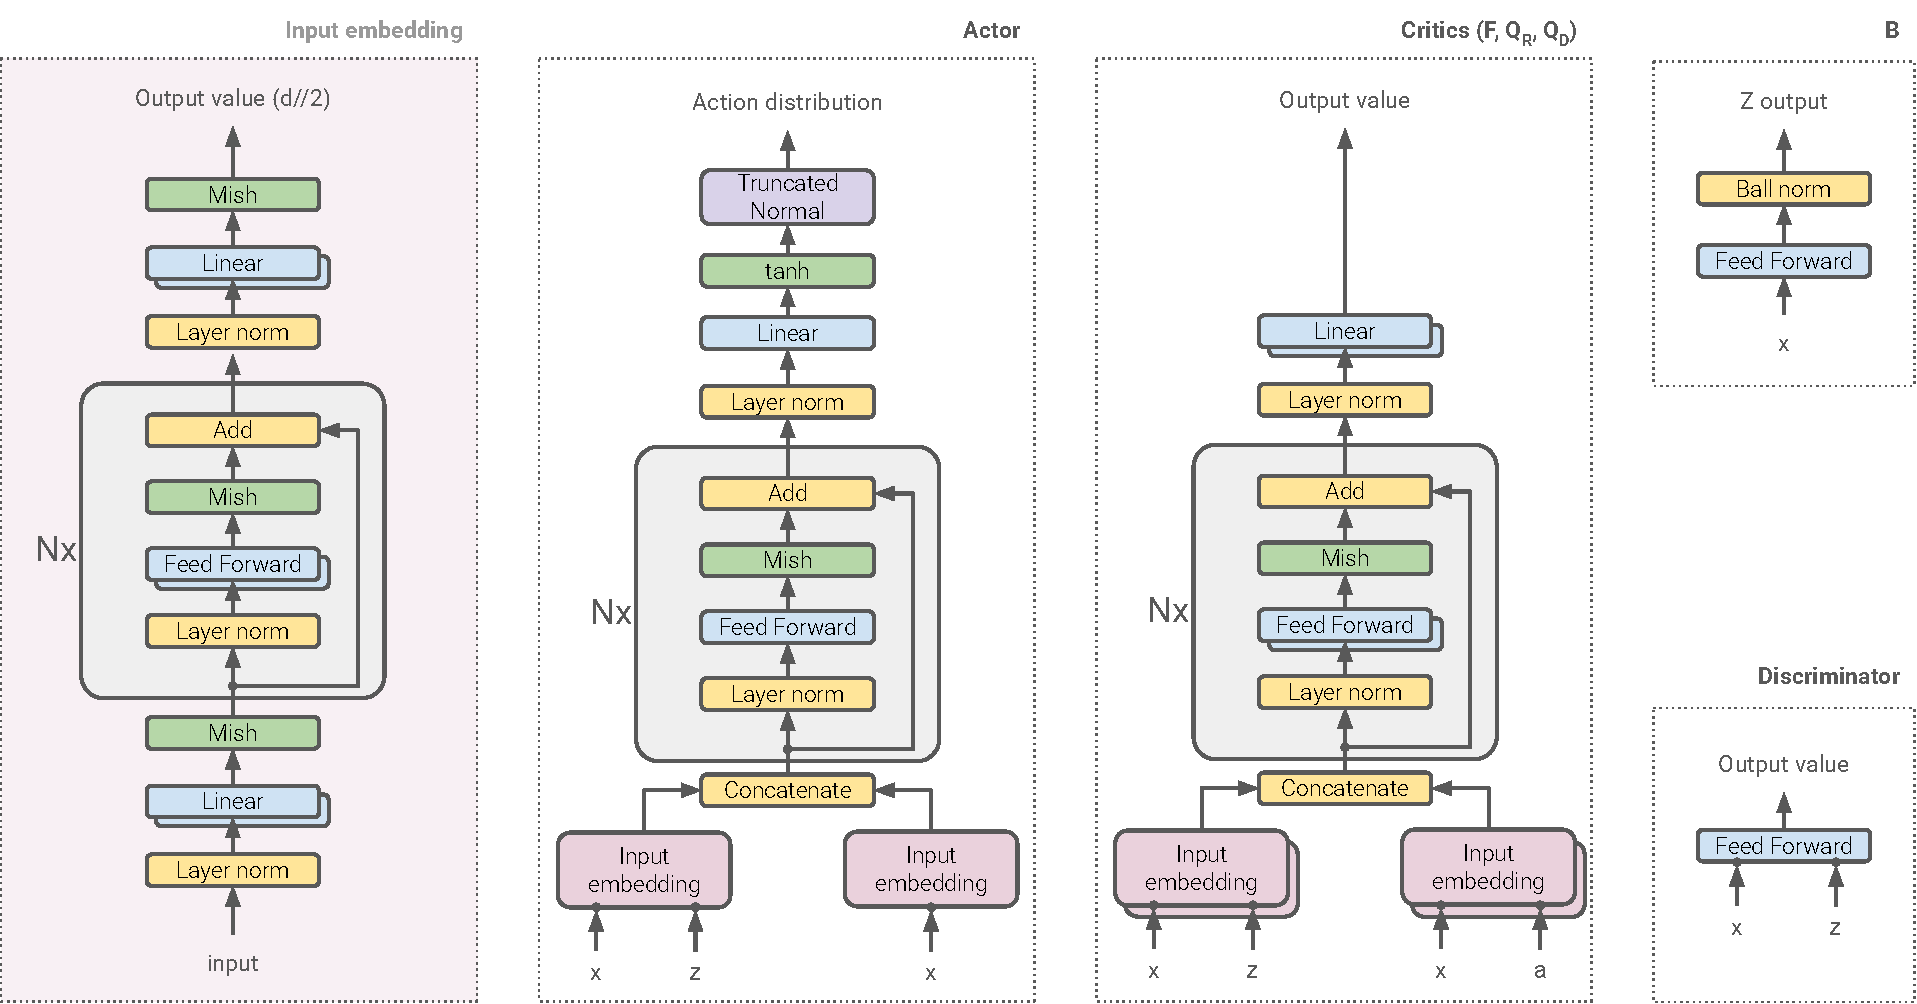
\includegraphics[width=0.99\linewidth]{image/architectures}
%     \caption{Visual representation of the network architectures.}
%     \label{fig:architectures}
%     \end{minipage}\\[.2in]
%     \begin{minipage}{\textwidth}
%     \centering
% \resizebox{.8\textwidth}{!}{%
%     \begin{tabular}{ccccc}
% \hline
% Hyperparameter & Critics (F, $Q_D$, $Q_R$)  & Actor & Discriminator & B\\
% \hline
% Input variables & $(x, a, z)$ & $(x, z)$ & $(x,z)$ & $(x)$\\
% Output dim & \makecell{F: $d$\\ $Q_D, Q_R$: 1} & 29 & 1 & $d$\\
% Observation variable $x$ & $(o_{t,H}, s_t)$ & $o_{t,H}$ & $(s_t,o_t)$ & $(s_t,o_t)$\\
% Embedding residual blocks & 4  & 4& - & -\\
% Embedding hidden units & 2048  &2048& - & -\\
% Residual blocks & 6 &  6  & - & -\\
% Feed Forward Hidden layers & 1& 1& 2 & 1\\
% Feed Forward Hidden units & 2048 & 2048 & 1024 & 256\\
% Activations & Mish &Mish& ReLu& ReLu\\
% Number of parallel networks & 2  & 1 & 1 & 1\\
% \hline
% \makecell{Number of parameters\\ (no target nets)} & \makecell{$F:135.8$M\\$Q_D, Q_R: 134.8$M} & $31.9$M & $2.9$M & $0.2$M\\
% Total number of parameters & \multicolumn{4}{c}{$846.2$M}\\
% \hline
% \end{tabular}
% }
% \caption{Network architecture parameters. We report the configuration used for real tests. Note that $s_t$ is the privileged information and $o_t$ is the proprioceptive information, $o_{t,H} = \{o_{t-H}, a_{t-H}, \ldots, o_t\}$ is the history composed by proprioceptive and action.}
% \label{tab:archi}
%     \end{minipage}
% \end{figure}


% \begin{table}[h]
% \centering
% \begin{tabular}{cccccc}
% \hline
% Hyperparameter & Critics (F, $Q_D$) & $Q_R$ & Actor & Discriminator & B\\
% \hline
% Input variables & $(x, a, z)$ &$(x, a, z)$ & $(x, z)$ & $(x,z)$ & $(x)$\\
% Output dim & F: $d$; $Q_D$: 1 & 1 & 29 & 1 & $d$\\
% Observation variable $x$ & $(h_t, s_t)$& $(h_t, s_t)$ & $h_t$ & $(s_t,o_t)$ & $(s_t,o_t)$\\
% Embedding residual blocks & 4 &  - & 4& - & -\\
% Embedding hidden units & 2048 & - &2048& - & -\\
% Residual blocks & 6 & - & 6  & - & -\\
% Feed Forward Hidden layers & 1 & 2& 1& 2 & 1\\
% Feed Forward Hidden units & 2048 & 1024 & 2048 & 1024 & 256\\
% Activations & Mish &  ReLu &Mish& ReLu& ReLu\\
% Number of parallel networks & 2 & 2 & 1 & 1 & 1\\
% \hline
% \end{tabular}
% \caption{Network architecture parameters. We report the configuration used for real tests. Note that $h_t$ is the history composed by proprioceptive and action, $s_t$ is the privileged information and $o_t$ is the proprioceptive information.}
% \label{tab:archi}
% \end{table}




\subsection{\method Algorithm Details}
We provide here a sketch of \method in (Alg.~\ref{alg:bfm.zero}). We report the algorithm without parallel networks for clarity. For clarity, we also report the FB loss here. Let $a'_i \sim \pi(x_i', z_i)$ where $x_i = (o_{i,H},s_i)$, then 
% \clearpage
\begin{equation}
\label{eq:fb.loss}
    \begin{aligned}
        \ell_{\mathrm{fb}} =&
        \frac{1}{2n(n-1)}  \sum_{i\neq k}\Big( F(x_i,a_i,z_i)^\top B(s_k',o_k')  - \gamma \overline{F}(x_i',a_i',z_i)^\top \overline{B}(s_k',o_k') \Big)^2\\
        & - \frac{1}{n} \sum_{i} F(x_i, a_i, z_i)^\top B(o'_{i}, s'_{i}) \\
        &+\frac{1}{2n(n-1)}  \sum_{i\neq k}\Big(B(s_i',o_i')^\top B(s_k',o_k')\Big)^2 - \frac{1}{n} \sum_{i\in[n]} B(s_i',o_i')^\top B(s_i',o_i')\\
        &+\frac{1}{n} \sum_{i\in[n]} \Big( F(x_i,a_i,z_i)^\top z_i - \overline{B}(s_i', o_i')\Sigma_{\overline{B}} z_i -\gamma \overline{F}(x_i',a_i',z_i)^\top z_i \Big)^2
    \end{aligned}
\end{equation}

\begin{algorithm}[h!]
	\caption{\method{} Pre-Training}\label{alg:bfm.zero}
\begin{footnotesize}
	\begin{algorithmic}[1]
    \State Initialize empty train buffer: $\mathcal{D}_{\mathrm{online}} \leftarrow \emptyset$
    \State Initialize expert buffer $\mathcal{M}$ with action-free trajectories
	\For{$t = 1, \dots$}
        \State {\scriptsize\color{YellowGreen}\textit{//Online interaction}}
        \State Sample $\boldsymbol{z}_t = \{z_e\}_{e=1}^{N_{\mathrm{env}}}\in \mathbb{R}^{N_{\mathrm{env}}\times d}$ (if needed)
        \State Execute $\boldsymbol{a}_t \sim \pi(\boldsymbol{o}_{t,H}, \boldsymbol{z}_t) \in \mathbb{R}^{N_{\mathrm{env}}\times A}$ in the \emph{simulated} environments
        \State Store $(\boldsymbol{s}_t, \boldsymbol{o}'_{t,H}, \boldsymbol{a}_t, \boldsymbol{s}_t', \boldsymbol{o}'_{t+1,H}, \boldsymbol{z}_t)$  in $\mathcal{D}_{\mathrm{online}}$

        \State {\scriptsize\color{YellowGreen}\textit{//Update}}
        \For{$j = 1, \dots, N_{\mathrm{ups}}$}
            \State Sample a batch of $n=N_{\mathrm{batch}}$ transitions $\{({o}_{i,H}, {s}_i, {a}_i, {o}_{i,H}', {s}_i', {z}_i)\}_{i=1}^{n}$ from $\mathcal{D}_{\mathrm{online}}$
            \State Sample a batch of $\frac{n}{T_{\mathrm{seq}} }$ sequences $\{(w_{j, 1}, w_{j, 2} \ldots, w_{j, T_{\mathrm{seq}}}) \}_{j=1}^{\frac{n}{T_{\mathrm{seq}} }}$ from $\mathcal{M}$ where $w = ({s}_t, {o}_t)$
            \State {\scriptsize\color{YellowGreen}\textit{//Encode expert and update discriminator}}
            \State $z_j \leftarrow \frac{1}{T_{\mathrm{seq}}} \sum_{t = 1}^{T_{\mathrm{seq}}} B(w_{j, t}) $ ; $z_j \leftarrow \sqrt{d} \frac{z_j}{\| z_j\|_2} $
            \State $\ell_{\mathrm{discriminator}} = - \frac{1}{n} \sum_{j = 1}^{\frac{n}{T_{\mathrm{seq}} }} \sum_{t = 1}^{T_{\mathrm{seq}}} \log D({w}_{j,t}, {z}_j) - \frac{1}{n} \sum_{i=1}^n \log (1-D({s}_i, {o}_i,{z}_i))$
            \State {\scriptsize\color{YellowGreen}\textit{//Update representation F and B so that } $F(s,a;z)^\top B(s') \approx M^{\pi_z}(ds'|s,a) $}
            \State Refer to Eq.~\ref{eq:fb.loss}
            \State {\scriptsize\color{YellowGreen}\textit{//note that $D$ does not use history}}
            \State Compute discriminator reward: $r_i^D \leftarrow \log (D({s}_i,{o}_i,  {z}_i)) - \log (1-D({s}_i,{o}_i,  {z}_i)), \quad \forall i \in [n]$
            \State Let $x_i = (o_{i,H}, s_i)$ and sample ${u}_i \sim \pi({o}_{i,H},{z}_i)$ for all $i\in[n]$. Then
            % \State {\scriptsize\color{YellowGreen}\textit{//Update critic $Q_D$}}
	        \State $\ell_{\texttt{critic}_D} =\frac{1}{n} \sum_{i\in[n]} \left( Q_{D}(x_i,{a}_i,{z}_i) - r_i^D - \gamma \overline{Q_D}(x_i',{a}_i,{z}_i) \right)^2$
            % \State {\scriptsize\color{YellowGreen}\textit{//Update critic $Q_R$}}
	        \State $\ell_{\texttt{critic}_R} =\frac{1}{n} \sum_{i\in[n]} \left( Q_{R}(x_i,{a}_i,{z}_i) - \sum_k r^{\mathrm{aux}}_k (x_i') - \gamma \overline{Q_R}(x_i',{a}_i,{z}_i) \right)^2$
            % \State {\scriptsize\color{YellowGreen}\textit{//Update actor }}
            \State $\ell_{\texttt{actor}} = -\frac{1}{n} \sum_{i\in[n]}\Big( F(x_i,{u}_i,{z}_i)^\top {z}_i  + \alpha_D Q_D(x_i,{u}_i,{z}_i) + \alpha_R Q_R(x_i,{u}_i,{z}_i)\Big)$
            \State {\scriptsize\color{YellowGreen}\textit{//Update target networks}}
        \EndFor
    \EndFor
	\end{algorithmic}
 \end{footnotesize}
	\end{algorithm}

\subsection{Training Environments}

To better facilitate sim-to-real transfer, we incorporated domain randomization, additive observation noise and regularization rewards in the training environment. Refer to Fig~\ref{fig:dr_and_reg} for details.

\begin{figure}[h]
\centering
\begin{tabular}{@{}c@{\hspace{2em}}c@{\hspace{2em}}c@{}}
% --- 左表：Dynamics Randomization ---
{
\footnotesize
\begin{tabular}[t]{lc}
\multicolumn{2}{c}{\textbf{Domain Randomization}} \\
\toprule
\textbf{Parameter} & \textbf{Range} \\
\midrule
COM Offset [m]            & $\mathcal{U}([-0.02, 0.02])$ \\
Link Mass             & $\mathcal{U}([0.95, 1.05])$ \\
Friction                        & $\mathcal{U}([-0.5, 1.25])$ \\
Default Joint Pos [m]    & $\mathcal{U}([-0.02, 0.02])$ \\
Push Robots [m/s]     & $\mathcal{U}([0, 0.5])$ \\
\bottomrule
\end{tabular}
}
&
% --- 中表：Observation Noise ---
{
\footnotesize
\begin{tabular}[t]{lc}
\multicolumn{2}{c}{\textbf{Additive Observation Noise}} \\
\toprule
\textbf{Observation} & \textbf{Range} \\
\midrule
$q_t - \bar{q}$                & $\mathcal{U}([-0.01, 0.01])$ \\
$\dot{q}_t$                    & $\mathcal{U}([-0.5, 0.5])$ \\
$\mathrm{grav}_t$              & $\mathcal{U}([-0.05, 0.05])$ \\
$\dot{\omega}^{\mathrm{root}}_t / 4$ & $\mathcal{U}([-0.05, 0.05])$ \\
\bottomrule
\end{tabular}
}
&
% --- 右表：Reward Regularization ---
{
\footnotesize
\begin{tabular}[t]{lc}
\multicolumn{2}{c}{\textbf{Regularization Rewards}} \\
\toprule
\textbf{Name} & \textbf{Weight} \\
\midrule
DoF Limit        & $-10$ \\
Action Rate      & $-0.1$ \\
Self Contact     & $-1$ \\
Feet Orientation & $-0.4$ \\
Ankle Roll       & $-4$ \\
Feet Slip        & $-2$ \\
\bottomrule
\end{tabular}
}
\end{tabular}
\caption{Details in training environment.}
\label{fig:dr_and_reg}
\end{figure}

\section{Tasks and Metrics}

In this section, we provide a complete description of the tasks and metrics.


\paragraph{Goal-based evaluation}
We have manually extracted $21$ ``stable'' poses (i.e., states with zero velocities) from the train dataset (i.e., LAFAN1) and $10$ poses from the test dataset (i.e., AMASS). We report the selected poses from LAFAN1 in Fig~\ref{fig:poses_lafan}. To evaluate how close is the agent to the goal pose, we use the joint error defined as following
\[
E_{\mathrm{mpjpe}}(e, g) = \frac{1}{|e|}\sum_{t=1}^{|e|} \|q_t(e) - q(g)\|_2
\]
where $e$ is an episode and $q$ is the joint position (i.e., 29D). We report the average across goals. The episodes are fixed in length $H=500$.

\begin{figure}[h]
    \centering
    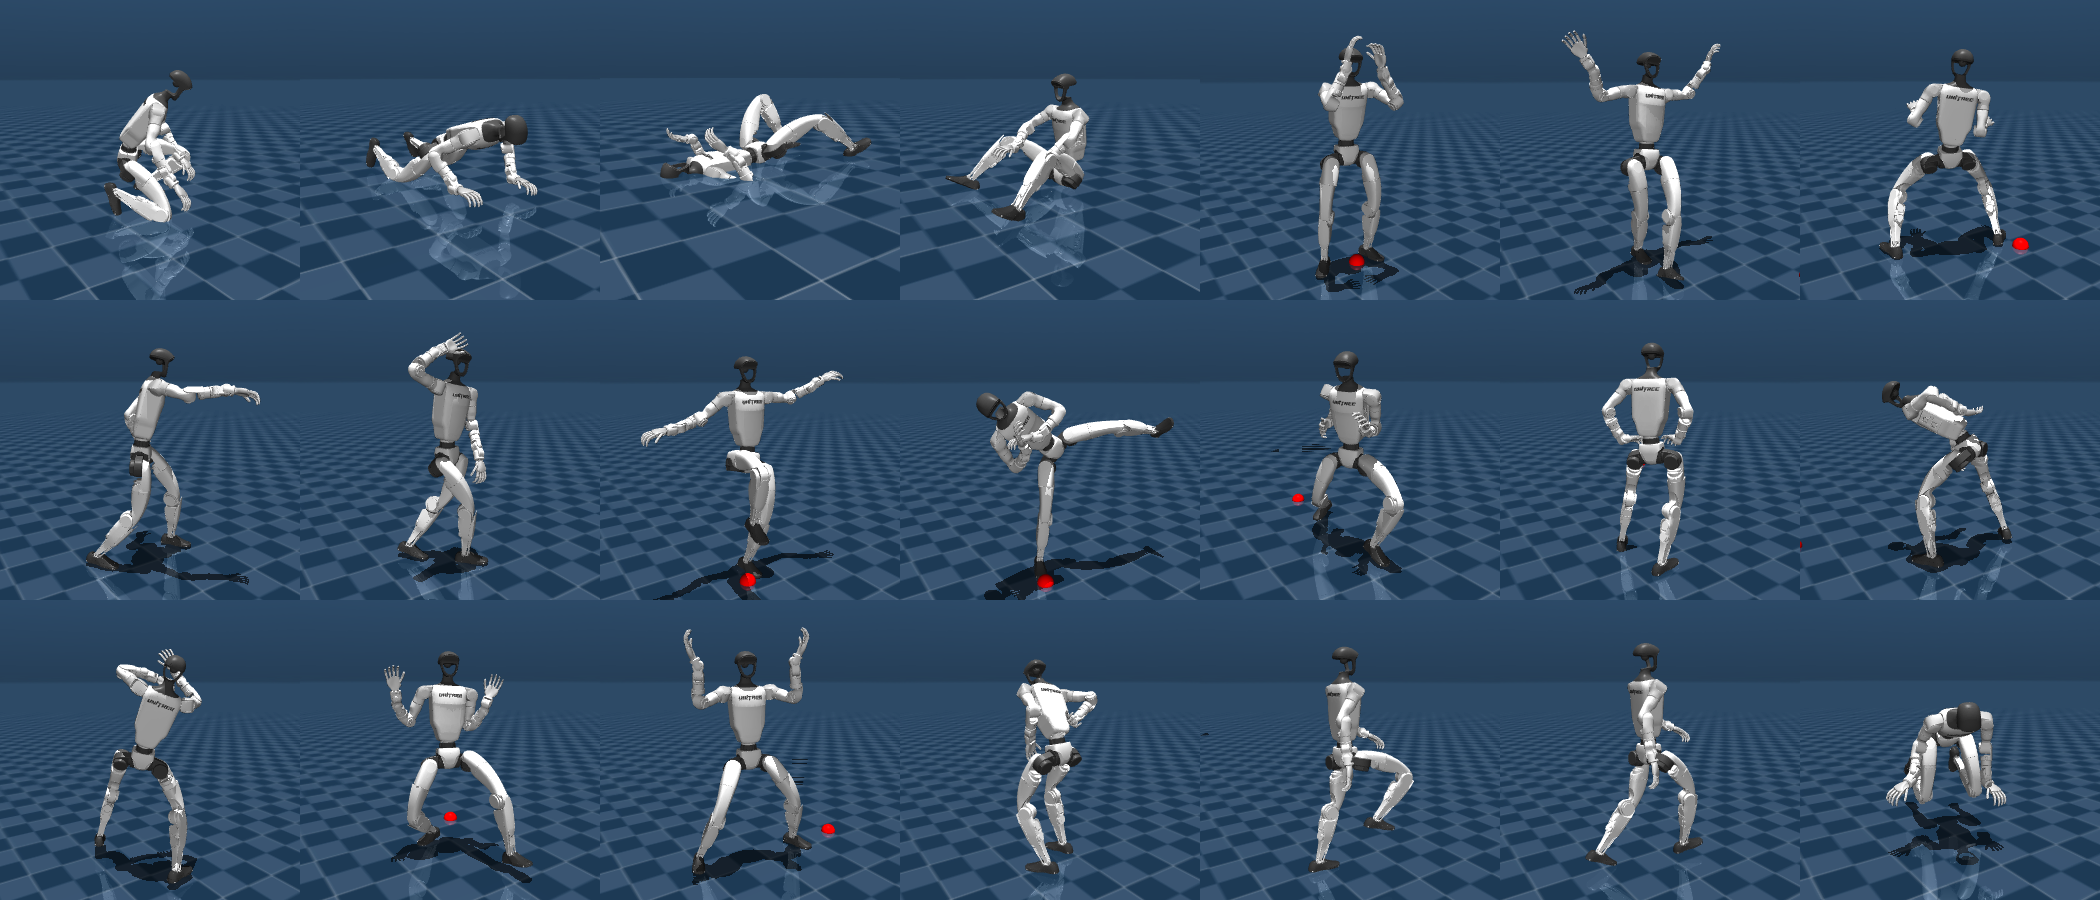
\includegraphics[width=.99\linewidth]{image/selected_goals_lafan29dof}
    \caption{Goal poses selected from frames of the LAFAN1 dataset~\citep{HarveyYNP20lafan1}.}
    \label{fig:poses_lafan}
\end{figure}

\paragraph{Tracking evaluation}
This evaluation aims to assess the ability of the model to imitate a sequence of poses, ideally matching both positions and velocities. We evaluate the agent both on the train dataset (i.e., LAFAN1) and on out-of-distribution motions selected from AMASS (retargeted to G1). In particular, we randomly selected $175$ motions from the CMU dataset of AMASS. For evaluation, we use the same metric as in goal evaluation, i.e.,
\[
E_{\mathrm{mpjpe}}(e, m) = \frac{1}{|e|}\sum_{t=1}^{|e|} \|q_t(e) - q_t(m)\|_2
\]
and we report the average across motions.

\paragraph{Reward evaluation}\label{app:rewards}
We define $6$ reward categories inspired by~\citep{TirinzoniTFGKXL25zeroshot}. The reward can be expressed as a function of the next state and normalized in $[0,1]$.

\textit{Standing}. We evaluate the agent's ability to stand with the pelvis at different heights. \texttt{move-ego-0-0} requires pelvis above 60cm and zero velocity, while \texttt{move-ego-low0.5-0-0} requires the pelvis to be between 50cm and 65cm.

\textit{Locomotion}. This category includes rewards related that requires the agent to move at a certain speed, in a certain direction and at a certain height. We consider $5$ representative rewards (\texttt{move-ego-0-0.7}, \texttt{move-ego-90-0.7}, \texttt{move-ego-(-90)-0.7}, \texttt{move-ego-0-0.3}, \texttt{move-ego-180-0.3}) which include forward, lateral and backward movement. We additionally test also walking forward but with the pelvis at a low height (\texttt{move-ego-low0.6-0-0.7}).

\textit{Rotation}. We require the robot to rotate along the vertical axis (i.e., while standing). We consider rotating clockwise and counterclockwise (i.e., \texttt{rotate-z-5-0.5} and \texttt{rotate-z-(-5)-0.5}).

\textit{Ground poses}. To further stress the ability of the model to control the vertical position, we define rewards requiring the agent to sit on the ground (\texttt{sitting}) or having the pelvis slightly above the ground (\texttt{crouch-0.25} is about 25cm above the ground).

\textit{Arm raise}. We require the robot to stand in a steady position and to reach a certain vertical position with the arms (measured at the wrists). We consider low ($z \in [0.6m, 0.8m]$) and medium ($z > 1m$) positions for the wrists, with soft margins (\texttt{raisearms-l-l}, \texttt{raisearms-l-m}, \texttt{raisearms-m-l}, \texttt{raisearms-m-m}).


\textit{Combined rewards.} We finally evaluate the ability of the agent to maximize rewards that require combining multiple skills. In particular, we test combinations of locomotion and rotation with arm movements. We selected $8$ combinations of rewards.


Overall, we tested $24$ rewards and evaluated perfomance via the cumulative
return over episodes of $T = 500$ steps. The initial state of an episode is the default pose.
\section{Additional Results}

\begin{figure}[h]
    \centering
    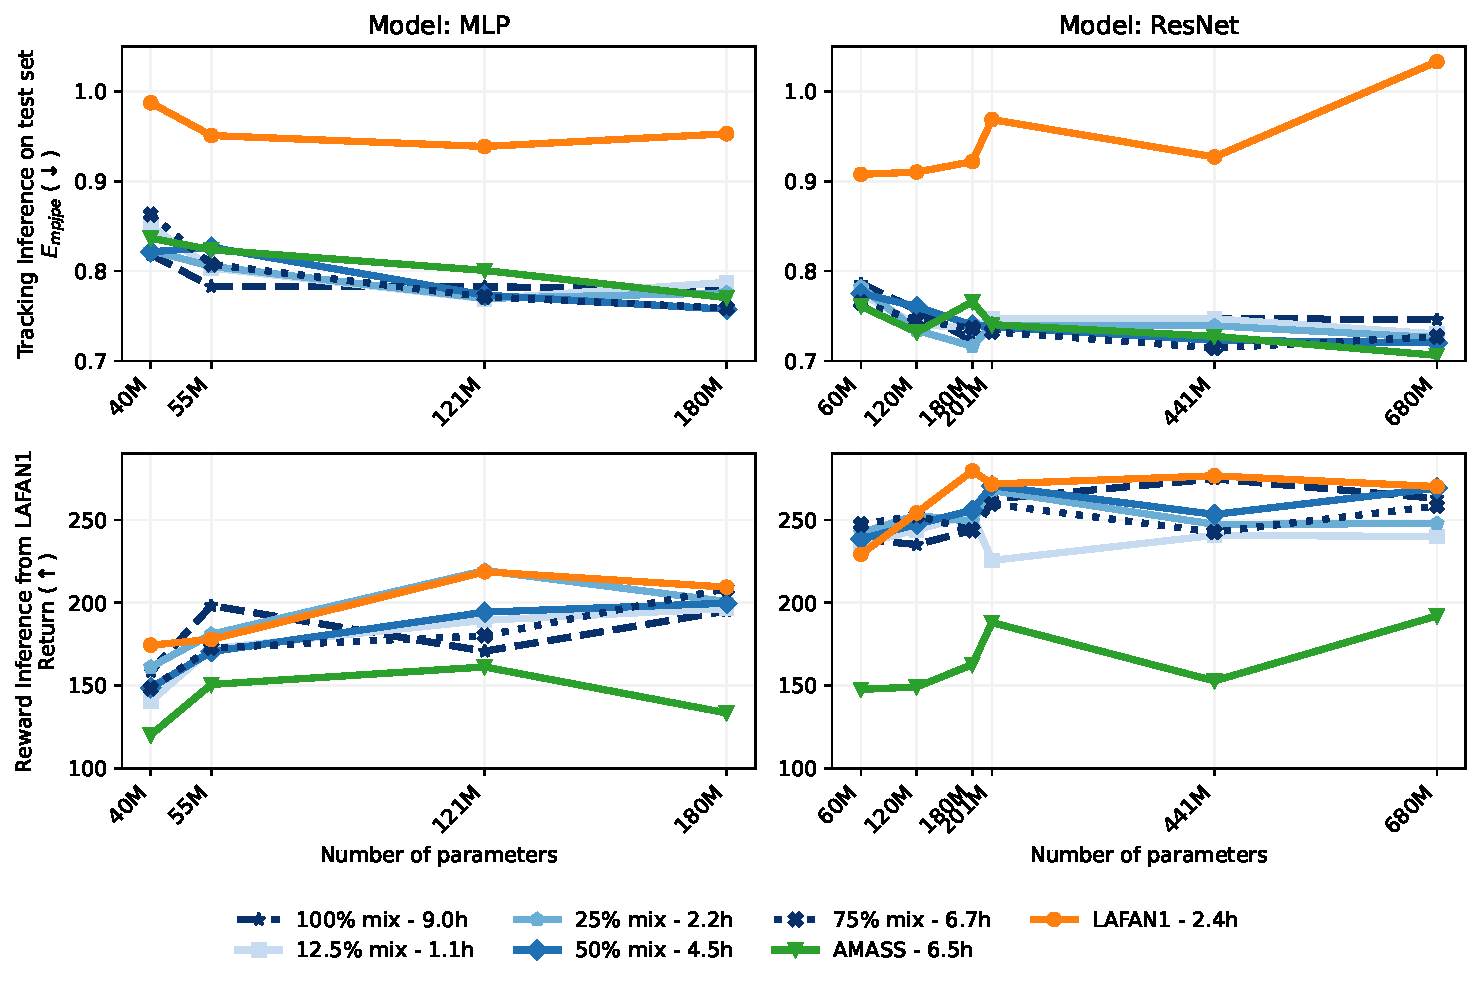
\includegraphics[width=0.96\linewidth]{image/scaling_plot_mix_linear.pdf}
    \caption{Tracking and reward performance on the test set for different models and datasets. The lower the better for tracking and the higher the better for reward.}
    \label{fig:scale_ablation}
\end{figure}

\subsection{Data Size and Model Size}
We perform ablations on both the data and model size. For training the model in the main paper, we used only the LAFAN1 dataset~\citep{HarveyYNP20lafan1}. In these ablations, we additionally leverage motions from the CMU and BMLHandball subsets of AMASS~\citep{Mahmood2019AMASS}. We consider the individual datasets (referred to as LAFAN1 and AMASS in the figure), as well as datasets obtained by merging $X$ percent of the two datasets (with $X = \{12.5\%,25\%,50\%, 75\%, 100\%\}$). We evaluate different network architectures, including simple feed-forward networks and residual architectures with a varying number of blocks (see Tab.~\ref{tab:config}). For tracking, we use the same test dataset as in~\citep{TirinzoniTFGKXL25zeroshot}, but we removed motions from CMU and BMLHandball to ensure complete separation from the training datasets. For reward inference, we use 600,000 samples from the LAFAN1 dataset for all configurations. We report the results of our ablation in Fig.~\ref{fig:scale_ablation} over a single seed.
\begin{table}[h]
\centering
\footnotesize
\begin{tabular}{|cc||cccccc|c|}
\hline
&& \multicolumn{7}{c|}{Number of Parameters}\\
\hline
Architecture & Model & $\pi$ & $Q_R$ & $B$ & $Q_D$ & D & F & Total\\
\hline
ResNet&3-block, 2048dim &19.3M&59.2M&201k&59.2M&2.9M&60.3M&201.1M\\
ResNet$^\star$&6-block, 2048dim &31.9M&134.8M&201k&134.8M&2.9M&135.9M&440.5M\\
ResNet&9-block, 2048dim &44.5M&210.4M&201k&210.4M&2.9M&211.5M&679.9M\\
ResNet&3-block, 1024dim &5.5M&17.0M&201k&17.0M&2.9M&17.6M&60.2M\\
ResNet&6-block, 1024dim &8.6M&36.0M&201k&36.0M&2.9M&36.5M&120.1M\\
ResNet&9-block, 1024dim &11.8M&54.9M&201k&54.9M&2.9M&55.4M&180.1M\\
\hline
MLP&2-layer, 1024dim &4.4M&10.7M&201k&10.7M&2.9M&11.2M&40.1M\\
MLP&2-layer, 2048dim &15.1M&34.0M&201k&34.0M&2.9M&35.0M&121.2M\\
MLP&4-layer, 1024dim &6.5M&14.9M&201k&14.9M&2.9M&15.4M&54.8M\\
MLP&4-layer, 2048dim &23.5M&50.8M&201k&50.8M&2.9M&51.8M&179.9M\\
\hline
\end{tabular}
\caption{Configurations of the architectures and total number of parameters. $\star$ denotes the configuration used in the main paper.}
\label{tab:config}
\end{table}

As we increase the total capacity of the model, tracking performance improves for almost all of the training mocap datasets. LAFAN1 is the only case where performance saturates quite early. We believe this is because the training dataset is a subset of the AMASS dataset, and despite being separated from the training data, it is likely much closer to the motions in CMU and BMLHandball than to those in LAFAN1. We can further notice that residual architectures achieve better performance w.r.t. simple MLP architectures, and we can scale residual architectures to larger sizes. Furthermore, we found training to be instable when scaling MLP to larger architectures.

% \begin{figure}[h]
%     \centering
%     \includegraphics[width=0.96\linewidth]{image/scaling_plot.png}
%     \caption{Tracking and reward performance on the test set for different models and datasets. The lower the better for tracking and the higher the better for reward. We use a log scale for the number of parameters and for the tracking score.}
%     \label{fig:scale_ablation}
% \end{figure}


Similarly, we observe a mild improvement trend for reward inference when increasing the model size. However, training with LAFAN1 (in some proportion) appears to be important in this case, as reward performance drops when we train only with the subset of AMASS. We also evaluated reward inference performance using both the training buffer and the training motion set. In both cases, the average performance decreases, with a much more significant drop when using the training buffer. We believe this may be due to the fact that samples in the buffer are collected with domain randomization, whereas the motion buffers are not randomized. Selecting the optimal dataset for reward inference could be an interesting direction for future research.

% \begin{figure}[h]
%     \centering
%     \includegraphics[width=0.96\linewidth]{image/scaling_plot_rewards.png}
%     \caption{}
%     \label{fig:scale_ablation_rewards}
% \end{figure}

\begin{figure}[h]
    \centering
    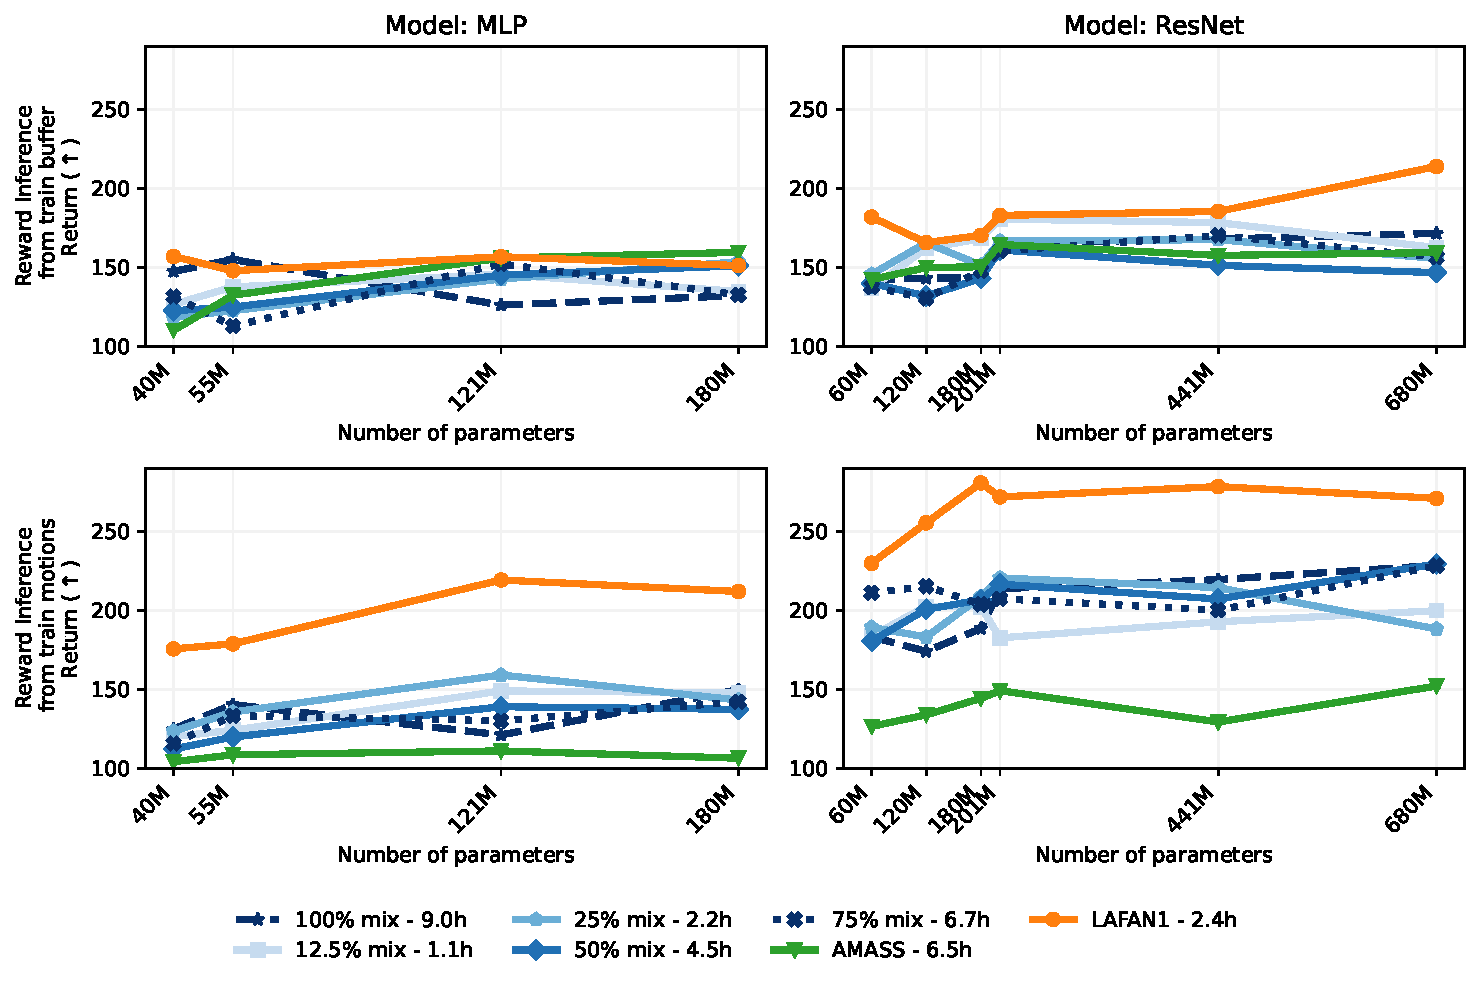
\includegraphics[width=0.96\linewidth]{image/scaling_plot_mix_reward_linear.pdf}
    \caption{Reward inference performance when using the experience generated by the agent (i.e., online replay buffer) or the motion dataset used for training. We get better reward performance when using the motion dataset, in particular when using LAFAN1 (see Fig.~\ref{fig:scale_ablation}).}
    \label{fig:scale_ablation_rewards}
\end{figure}

% \clearpage
\subsection{Application of \method{} on Booster T1}
\label{sec:t1-sim}
We additionally evaluate the generality of our framework by testing \method{} on Booster T1 humanoid robot. The LAFAN1 dataset is retargeted to T1 using LocoMujoco~\citep{alhafez2023b} and we train the policy with exact same hyper-parameters as G1. The algorithm shows strong generalization ability, allowing T1 also to perform natural walking and expressive dancing motions, as shown in~\Cref{fig:t1-sim}.
\begin{figure}[t]
    \centering
    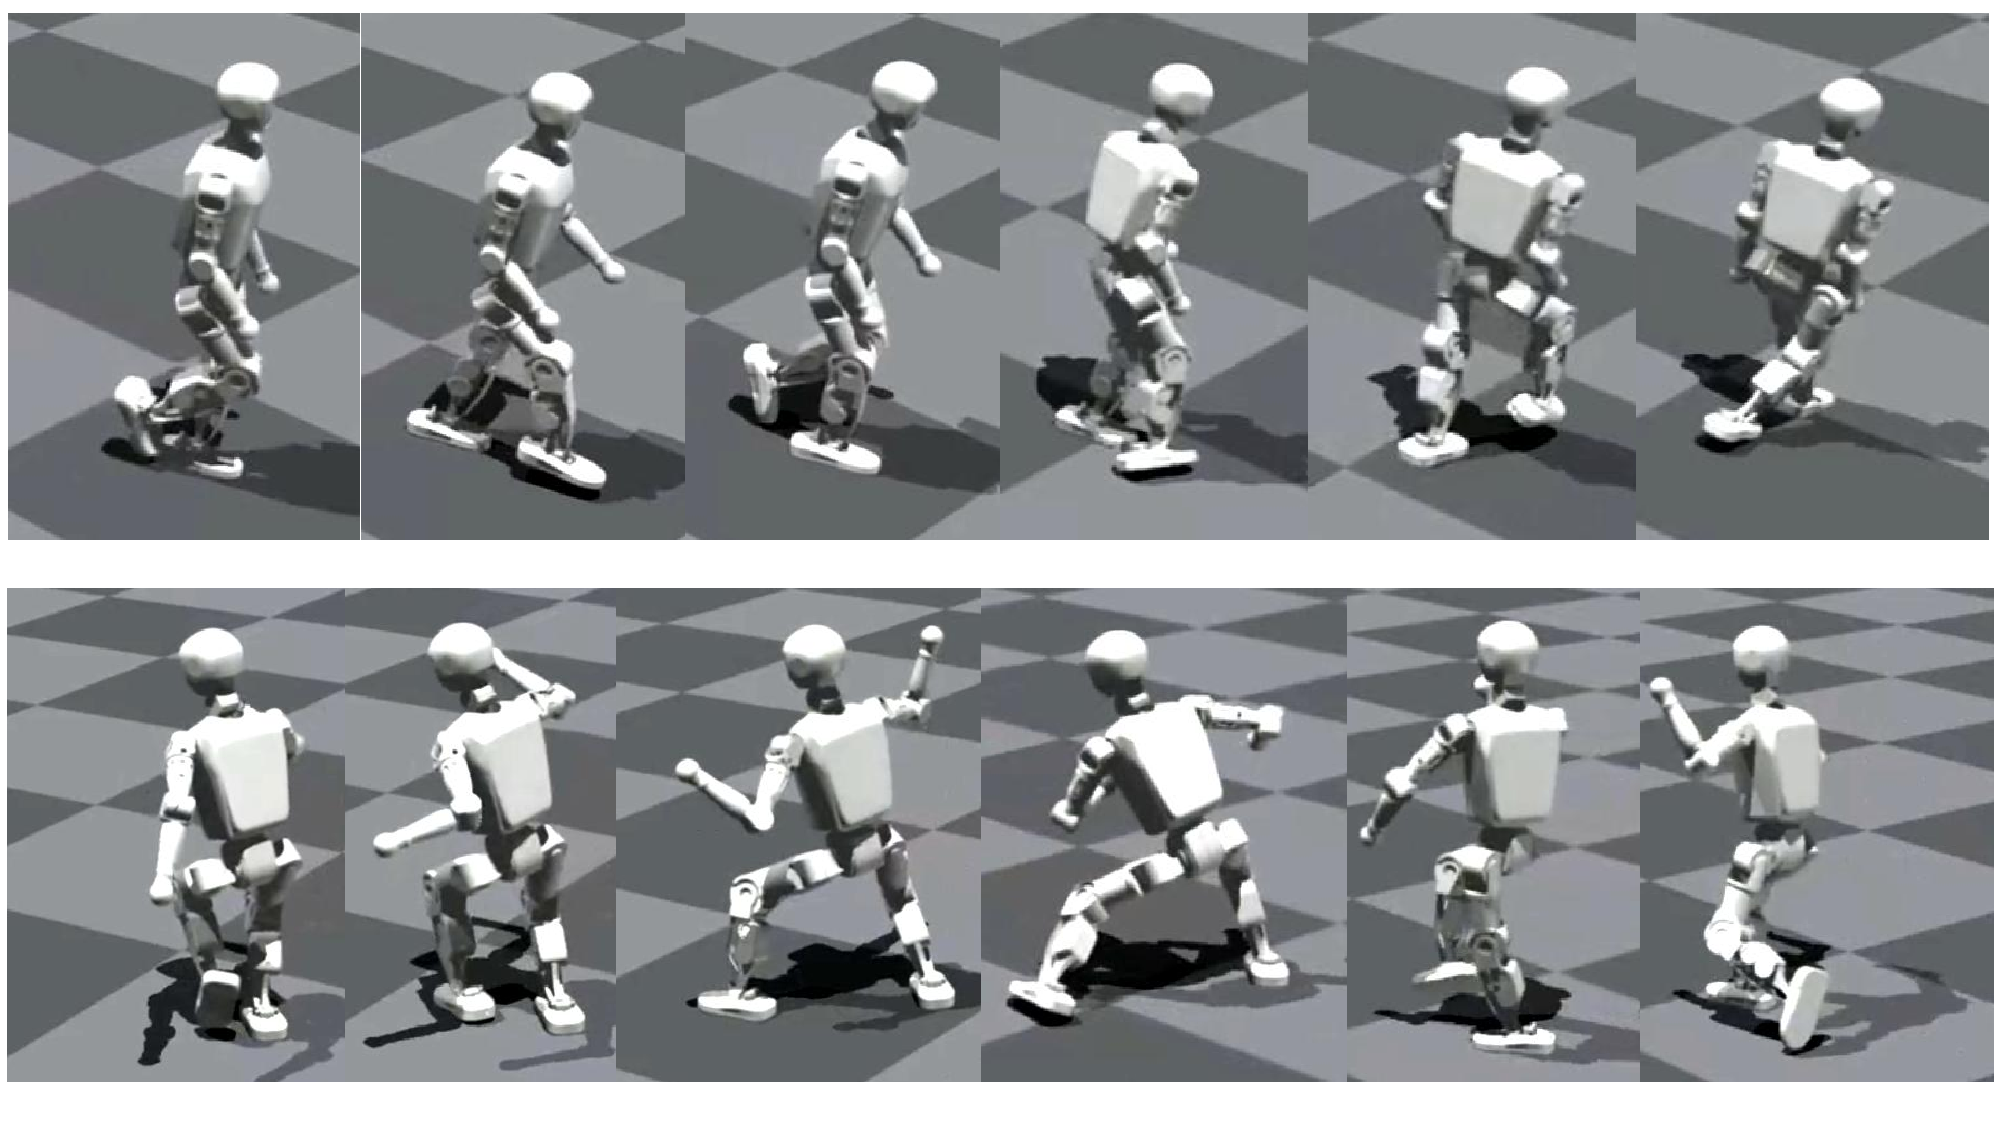
\includegraphics[width=0.7\linewidth]{image/t1_sim.pdf}
    \caption{Application of \method{} on Booster T1.}
    \label{fig:t1-sim}
\end{figure}


% \section{Use of Large Language Models}
% The authors use LLM tools for refining the expression in the final draft of the paper, but did not use it for idea generation, training, and other experiments.


\end{document}